\documentclass[a4paper,12pt]{article}

\newcommand{\me}{Jonathan R.\ J.\ Yong}
\newcommand{\meshort}{J.R.J.Y.}
\newcommand{\eriks}{{\=E}riks Kup{\v{c}}e}
\newcommand{\tim}{Tim D. W. Claridge}

% Fonts {{{1
\usepackage{fontspec,amsmath,unicode-math}
\setmainfont[
  Path={./fonts/},
  Extension=.otf,
  UprightFont={*-regular},
  BoldFont={*-semibold},
  ItalicFont={*-italic},
  BoldItalicFont={*-semibolditalic},
  Ligatures=TeX,
]{minion3}
\setmonofont[
  Path={./fonts/},
  Extension=.ttf,
  UprightFont={*-Regular},
  BoldFont={*-SemiBold},
  ItalicFont={*-Italic},
  BoldItalicFont={*-SemiBoldItalic},
  Scale=MatchLowercase
]{RobotoMono}
\setmathfont[
  Path={./fonts/},
  Scale=MatchLowercase
]{MinionMath-Regular.otf}
% Other optical sizes for Minion
\newfontfamily{\fontcaption}{minion3caption}[
  Path={./fonts/},
  Extension=.otf,
  UprightFont={*-regular},
  BoldFont={*-semibold},
  ItalicFont={*-italic},
  BoldItalicFont={*-semibolditalic},
  Ligatures=TeX,
]
\newfontfamily{\fontsubhead}{minion3subhead}[
  Path={./fonts/},
  Extension=.otf,
  UprightFont={*-regular},
  BoldFont={*-bold},
  ItalicFont={*-italic},
  BoldItalicFont={*-bolditalic},
  Ligatures=TeX,
]
\usepackage[final]{microtype}
% }}}1
% Packages and settings {{{1
\usepackage[font=small,labelfont=it,margin=15pt,skip=5pt]{caption}
\usepackage{fullpage,parskip,graphicx,float,braket,setspace,subcaption,booktabs}
\usepackage[svgnames]{xcolor}
\usepackage{minted}
\usepackage{tcolorbox}
\tcbuselibrary{minted}
\renewcommand{\MintedPygmentize}{./pygmentize_bruker.py}
\usepackage{listings}
\lstset{upquote=true}
\newtcblisting{tcbminted}[1]{%
    colframe=black,%
    colback=white,%
    width=0.95\textwidth,%
    center,%
    listing only,%
    minted options={curlyquotes=false,fontsize=\small},%
    minted language={#1},%
}
\usepackage{chemformula}
\setchemformula{math-scripts=true}
\usepackage[style=chem-acs,subentry,articletitle,doi]{biblatex}
\addbibresource{abbs.bib}
\graphicspath{{./figures/}}
\usepackage{xurl}   % must be after biblatex
\usepackage[
  mode=match,
  range-phrase={--},
  range-units=single,
  propagate-math-font=true,
  reset-math-version=false,
  reset-text-family=false,
  reset-text-series=false,
  text-family-to-math=true,
  text-series-to-math=true
]{siunitx}
\usepackage[symbol]{footmisc}
\usepackage{titletoc}
\usepackage{hyperref}
\hypersetup{
    naturalnames,
    colorlinks,
    linkcolor={red!50!black},
    citecolor={blue!60!black},
    urlcolor={blue!80!black}
}
\usepackage[capitalise,noabbrev]{cleveref}
\usepackage{usebib}
\newbibfield{entryset}
\bibinput{abbs}
\onehalfspacing
\DeclareSIUnit{\molar}{\textsc{m}}
\DeclareSIUnit{\ppm}{ppm}
% }}}1
% Newcommands {{{1 
\DeclareMathOperator*{\sgn}{sgn}
\newcommand{\articletitle}{A General Scheme for NMR Supersequences Combining High- and Low-Sensitivity Experiments}
\newcommand{\crl}{Chemistry Research Laboratory, Department of Chemistry, University of Oxford, Mansfield Road, Oxford OX1 3TA, United Kingdom}
\newcommand{\turing}{The Alan Turing Institute, The British Library, 96 Euston Road, London NW1 2DB, United Kingdom}
\newcommand{\brukeruk}{Bruker UK Ltd, R\&D, Coventry CV4 9GH, United Kingdom}
\newcommand{\exscientia}{Exscientia Ltd, The Schr{\"o}dinger Building, Oxford Science Park, Oxford OX4 4GE, United Kingdom}
\newcommand{\proton}{\ch{^{1}H}}
\newcommand{\carbonbulk}{\ch{^{12}C}}
\newcommand{\carbon}{\ch{^{13}C}}
\newcommand{\nitrogen}{\ch{^{15}N}}
\newcommand{\SInf}{\textit{Supplementary Information}}
\newcommand{\CH}{\carbon{}--\proton{}}
\newcommand{\HC}{\proton{}--\carbon{}}
\newcommand{\NH}{\nitrogen{}--\proton{}}
\newcommand{\HN}{\proton{}--\nitrogen{}}
\newcommand{\HH}{\proton{}--\proton{}}
\newcommand{\magn}[1]{\ch{^1H}$^{#1}$}
\newcommand{\magnnot}[1]{\ch{^1H}$^{!#1}$}
\newcommand{\todo}[1]{{\color{OrangeRed}#1}}
\newcommand{\changed}[1]{{\color{DodgerBlue!75!blue}#1}}
\newcommand{\autociteset}[1]{\autocite{\usebibentry{#1}{entryset}}}
\newcommand{\onejch}{{}^1\!J_{\ch{CH}}}
\newcommand{\onejcc}{{}^1\!J_{\ch{CC}}}
\newcommand{\onejnh}{{}^1\!J_{\ch{NH}}}
\newcommand{\onejxh}{{}^1\!J_{\ch{XH}}}
\newcommand{\njch}{{}^n\!J_{\ch{CH}}}
\newcommand{\njcc}{{}^n\!J_{\ch{CC}}}
\newcommand{\njnh}{{}^n\!J_{\ch{NH}}}
\newcommand{\njxh}{{}^n\!J_{\ch{XH}}}
\newcommand{\theurl}{\url{https://nmr-genesis.co.uk}}
\newcommand*{\brucine}{Spectra were obtained on a \SI{700}{\MHz} Bruker AV III equipped with a TCI H/C/N cryoprobe; the sample used was \SI{50}{\milli\molar} brucine in \ch{CDCl3}}
\newcommand*{\cyclo}{Spectra were obtained on a \SI{700}{\MHz} Bruker AV III equipped with a TCI H/C/N cryoprobe; the sample used was \SI{50}{\milli\molar} cyclosporin A in \ch{C6D6}}
\newcommand{\angang}[2]{#1\rlap{\unit{\degree}}\ensuremath{_{#2}}}
% }}}1
% NOAH macros {{{1
\newcommand{\abn}{NOAH-2 AB$_{\ch{N}}$}
\newcommand{\abnbn}{NOAH-3 A(B$_{\ch{N}}$/B$_{\ch{N}}$)}
\newcommand{\abnbs}{NOAH-4 A(B$_{\ch{N}}$/B/S)}
\newcommand{\abnns}{NOAH-4 A(B$_{\ch{N}}$/N/S)}
\newcommand{\abnbspns}{NOAH-5 A(B$_{\ch{N}}$/B/S$^{+}_{\ch{N}}$/S)}
\ExplSyntaxOn
\msg_new:nnn{noah}{module-not-found}{Module~code~`#1'~not~recognised.~If~it~was~not~a~typo,~you~may~need~to~define~this~in~\c_backslash_str noahmodule.}
\NewDocumentCommand{\noahmodule}{m}{
    \str_case:nnTF{#1}{
        {A}{A}
        {Bn}{B${}\sb{\ch{N}}$}
        {B}{B}
        {Cc}{C$\sp{\text{c}}$}
        {Cqf}{C$\sp{\text{qf}}$}
        {C}{C}
        {D}{C}
        {Jqf}{J$\sp{\text{qf}}$}
        {J}{J}
        {Mn}{M$\sb{\ch{N}}$}
        {M}{M}
        {N}{N}
        {O}{O}
        {Pt}{P$\sp{\text{T}}$}
        {P}{P}
        {R}{R}
        {Sc}{S$\sp{\text{C}}$}
        {Sn}{S$\sb{\ch{N}}$}
        {Spa}{S$\sp+\sb1$}
        {Spb}{S$\sp+\sb2$}
        {Spn}{S$\sp{+}\sb{\ch{N}}$}
        {Sp}{S$\sp+$}
        {St}{S$\sp{\text{T}}$}
        {S}{S}
        {T}{T}
        {X}{X}
        }{}{\textbf{?}
        \msg_error:nnn{noah}{module-not-found}{#1}}
}
\NewDocumentCommand{\noah}{s m}{
    \IfBooleanTF{#1}{}{NOAH-\clist_count:n{#2}~}
    {\clist_map_inline:nn{#2}{\noahmodule{##1}}}
}
\ExplSyntaxOff
% }}}1

\begin{document} \begin{refsection}

\begin{center}   % Front matter
    \textbf{\Large \articletitle{}}

    \vspace{0.2cm}

    \me{},\textsuperscript{1} \eriks{},\textsuperscript{2} \tim\textsuperscript{1,\texttt{*}}

    \vspace{0.2cm}

    \small

    \textsuperscript{1} \textit{\crl{}}

    % \textsuperscript{2} \textit{\turing{}}

    \textsuperscript{2} \textit{\brukeruk{}}

    % \textsuperscript{4} \textit{\exscientia{}}

    \normalsize \textsuperscript{\texttt{*}} \texttt{tim.claridge@chem.ox.ac.uk}

    \vspace{0.5cm} \hrule

\end{center}

\small{
    \url{https://www.rsc.org/journals-books-databases/about-journals/chemcomm#writing-guidelines}

    \url{https://www.rsc.org/journals-books-databases/author-and-reviewer-hub/authors-information/prepare-and-format/}
}

\begin{figure*}[ht]
    \centering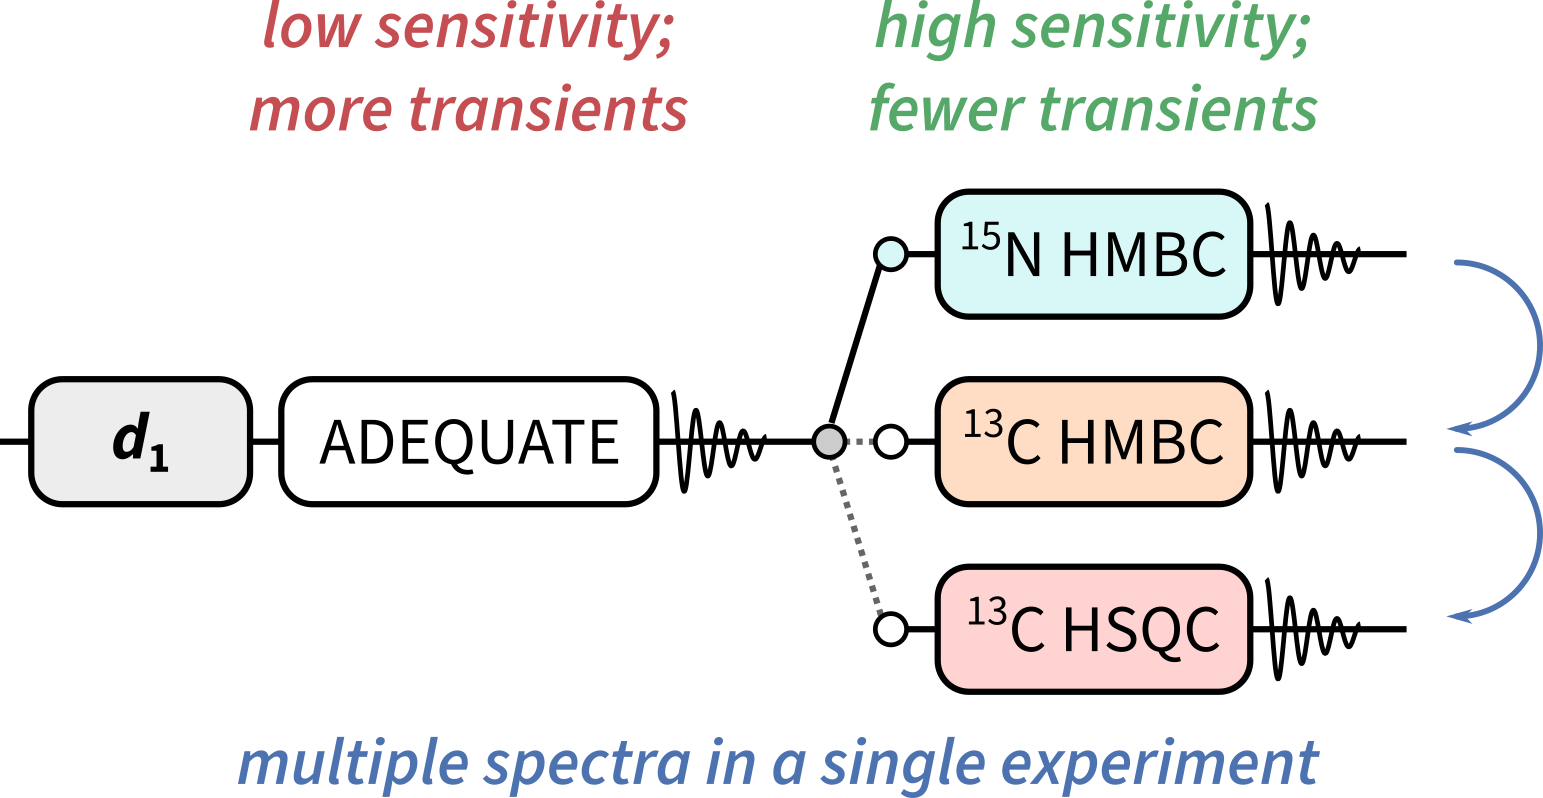
\includegraphics{toc.png}%

    The concept of NMR supersequences is generalised to allow 2D experiments with vastly different sensitivities to be combined, including 1,1-ADEQUATE, \nitrogen{} HMBC, and other heteronuclear experiments.
\end{figure*}

\section*{Abstract}

NOAH supersequences are a way of collecting multiple 2D NMR experiments in a single measurement.
So far, this approach has been limited to experiments with comparable sensitivity.
Here, we propose a scheme which overcomes this limitation, combining experiments with very different sensitivities such as 1,1-ADEQUATE, \nitrogen{} HMBC, and \carbon{} HSQC.

\section{Introduction}

Nuclear magnetic resonance (NMR) spectroscopy plays a key role in the structural elucidation of natural products; in particular, two-dimensional (2D) NMR experiments provide vast amounts of information on through-bond and through-space molecular connectivity.\autociteset{textbooks}
However, these experiments are often time-consuming as they require the incrementation of indirect-dimension evolution periods in order to construct the requisite 2D data matrices.
One particularly flexible method for accelerating 2D data acquisition is the NOAH (NMR by Ordered Acquisition using \proton{} detection) technique\autocite{Kupce2017ACIE,Kupce2021NRMP}, in which multiple 2D experiments (`modules') are combined into a single experiment using only a single recovery delay.
These nested `supersequences', which rely on the tailored excitation of magnetisation from different isotopologues, provide an array of 2D spectra (up to 10 so far\autocite{Kupce2021JACSA}) in greatly reduced experiment times.

Virtually all common 2D experiments, such as HSQC, HMQC, COSY, TOCSY, and NOESY, have been exploited in NOAH supersequences, allowing for the (manual or computer-assisted) structural elucidation of a wide range of molecules.\autocite{Kupce2018CC,Kupce2019JMR,Kupce2021JACSA,Yong2022AC}
However, such experiments tend to fall short in proton-sparse molecules\autociteset{proton_sparse} as they do not yield sufficient correlations.
In such cases, additional information may be obtained through the HMBC\autociteset{all_hmbc} and HSQMBC\autocite{Williamson2014JOC,Castanar2014ACIE} experiments which detect long-range X--\proton{} couplings ($\njxh{}$, X = \carbon{} or \nitrogen{}).
Although these tend to yield vastly more correlations, there may remain ambiguity in interpreting the resulting data as these techniques do not reveal the exact number of bonds over which a coupling is mediated.
In contrast, one-bond \carbon{}--\carbon{} correlations ($\onejcc$), obtained through the INADEQUATE\autocite{Bax1981JACS}---or more practically, ADEQUATE\autociteset{adequate}---experiments, allow chemists to directly trace out carbon backbones with much greater certainty.
The main limitation of such experiments is their low sensitivity, as they rely on pairs of heteronuclei with low natural abundances; nonetheless, with the introduction of cryogenically cooled probes and concomitant advances in achievable signal-to-noise ratios (SNRs), such experiments can nowadays be feasibly run even on relatively dilute samples.

To date, insensitive experiments such as \nitrogen{} HMBC and ADEQUATE have not been the main focus of NOAH supersequences.\autocite{RaoKakita2020RSCA}
This is because in a traditional `linear' supersequence, each constituent module is recorded with the same number of transients.
For dilute samples, the total experiment duration is therefore dictated by the module with the lowest sensitivity, and higher-sensitivity modules (e.g.\ HSQC or COSY) would be recorded with more transients than strictly necessary.
Although the more sensitive modules would still be obtained `for free', the \textit{effective} time savings thus realised are smaller than for a supersequence constructed from modules with balanced sensitivities.

For this reason, the low-sensitivity ADEQUATE and \nitrogen{} HMBC modules (respectively abbreviated as `\noah*{A}' and `\noah*{Bn}') form a `natural' pairing in the \abn{} supersequence introduced here (\cref{fig:sequences_ab}).
However, in this work, we also go beyond the traditional `linear' or `horizontal' model of a supersequence in adding more modules through `vertical' interleaving, in a similar fashion to the parallel supersequences recently described.\autocite{Kupce2021JACSA}
We show that, following an initial ADEQUATE module, up to four modules (\nitrogen{} HMBC, \carbon{} HMBC, \nitrogen{} sensitivity-enhanced HSQC (seHSQC), and \carbon{} HSQC) may be interleaved in this `vertical' fashion (\cref{fig:sequences_abbs,fig:sequences_abbss}), yielding five modules with balanced intensities and high-quality data.
By tailoring the number of times each module is acquired, this technique provides a powerful and flexible way to balance modules with different sensitivities, and fully generalises our previous work on parallel supersequences, which only `vertically' interleaved two modules at a time.

\begin{figure}[ht]
    \centering
    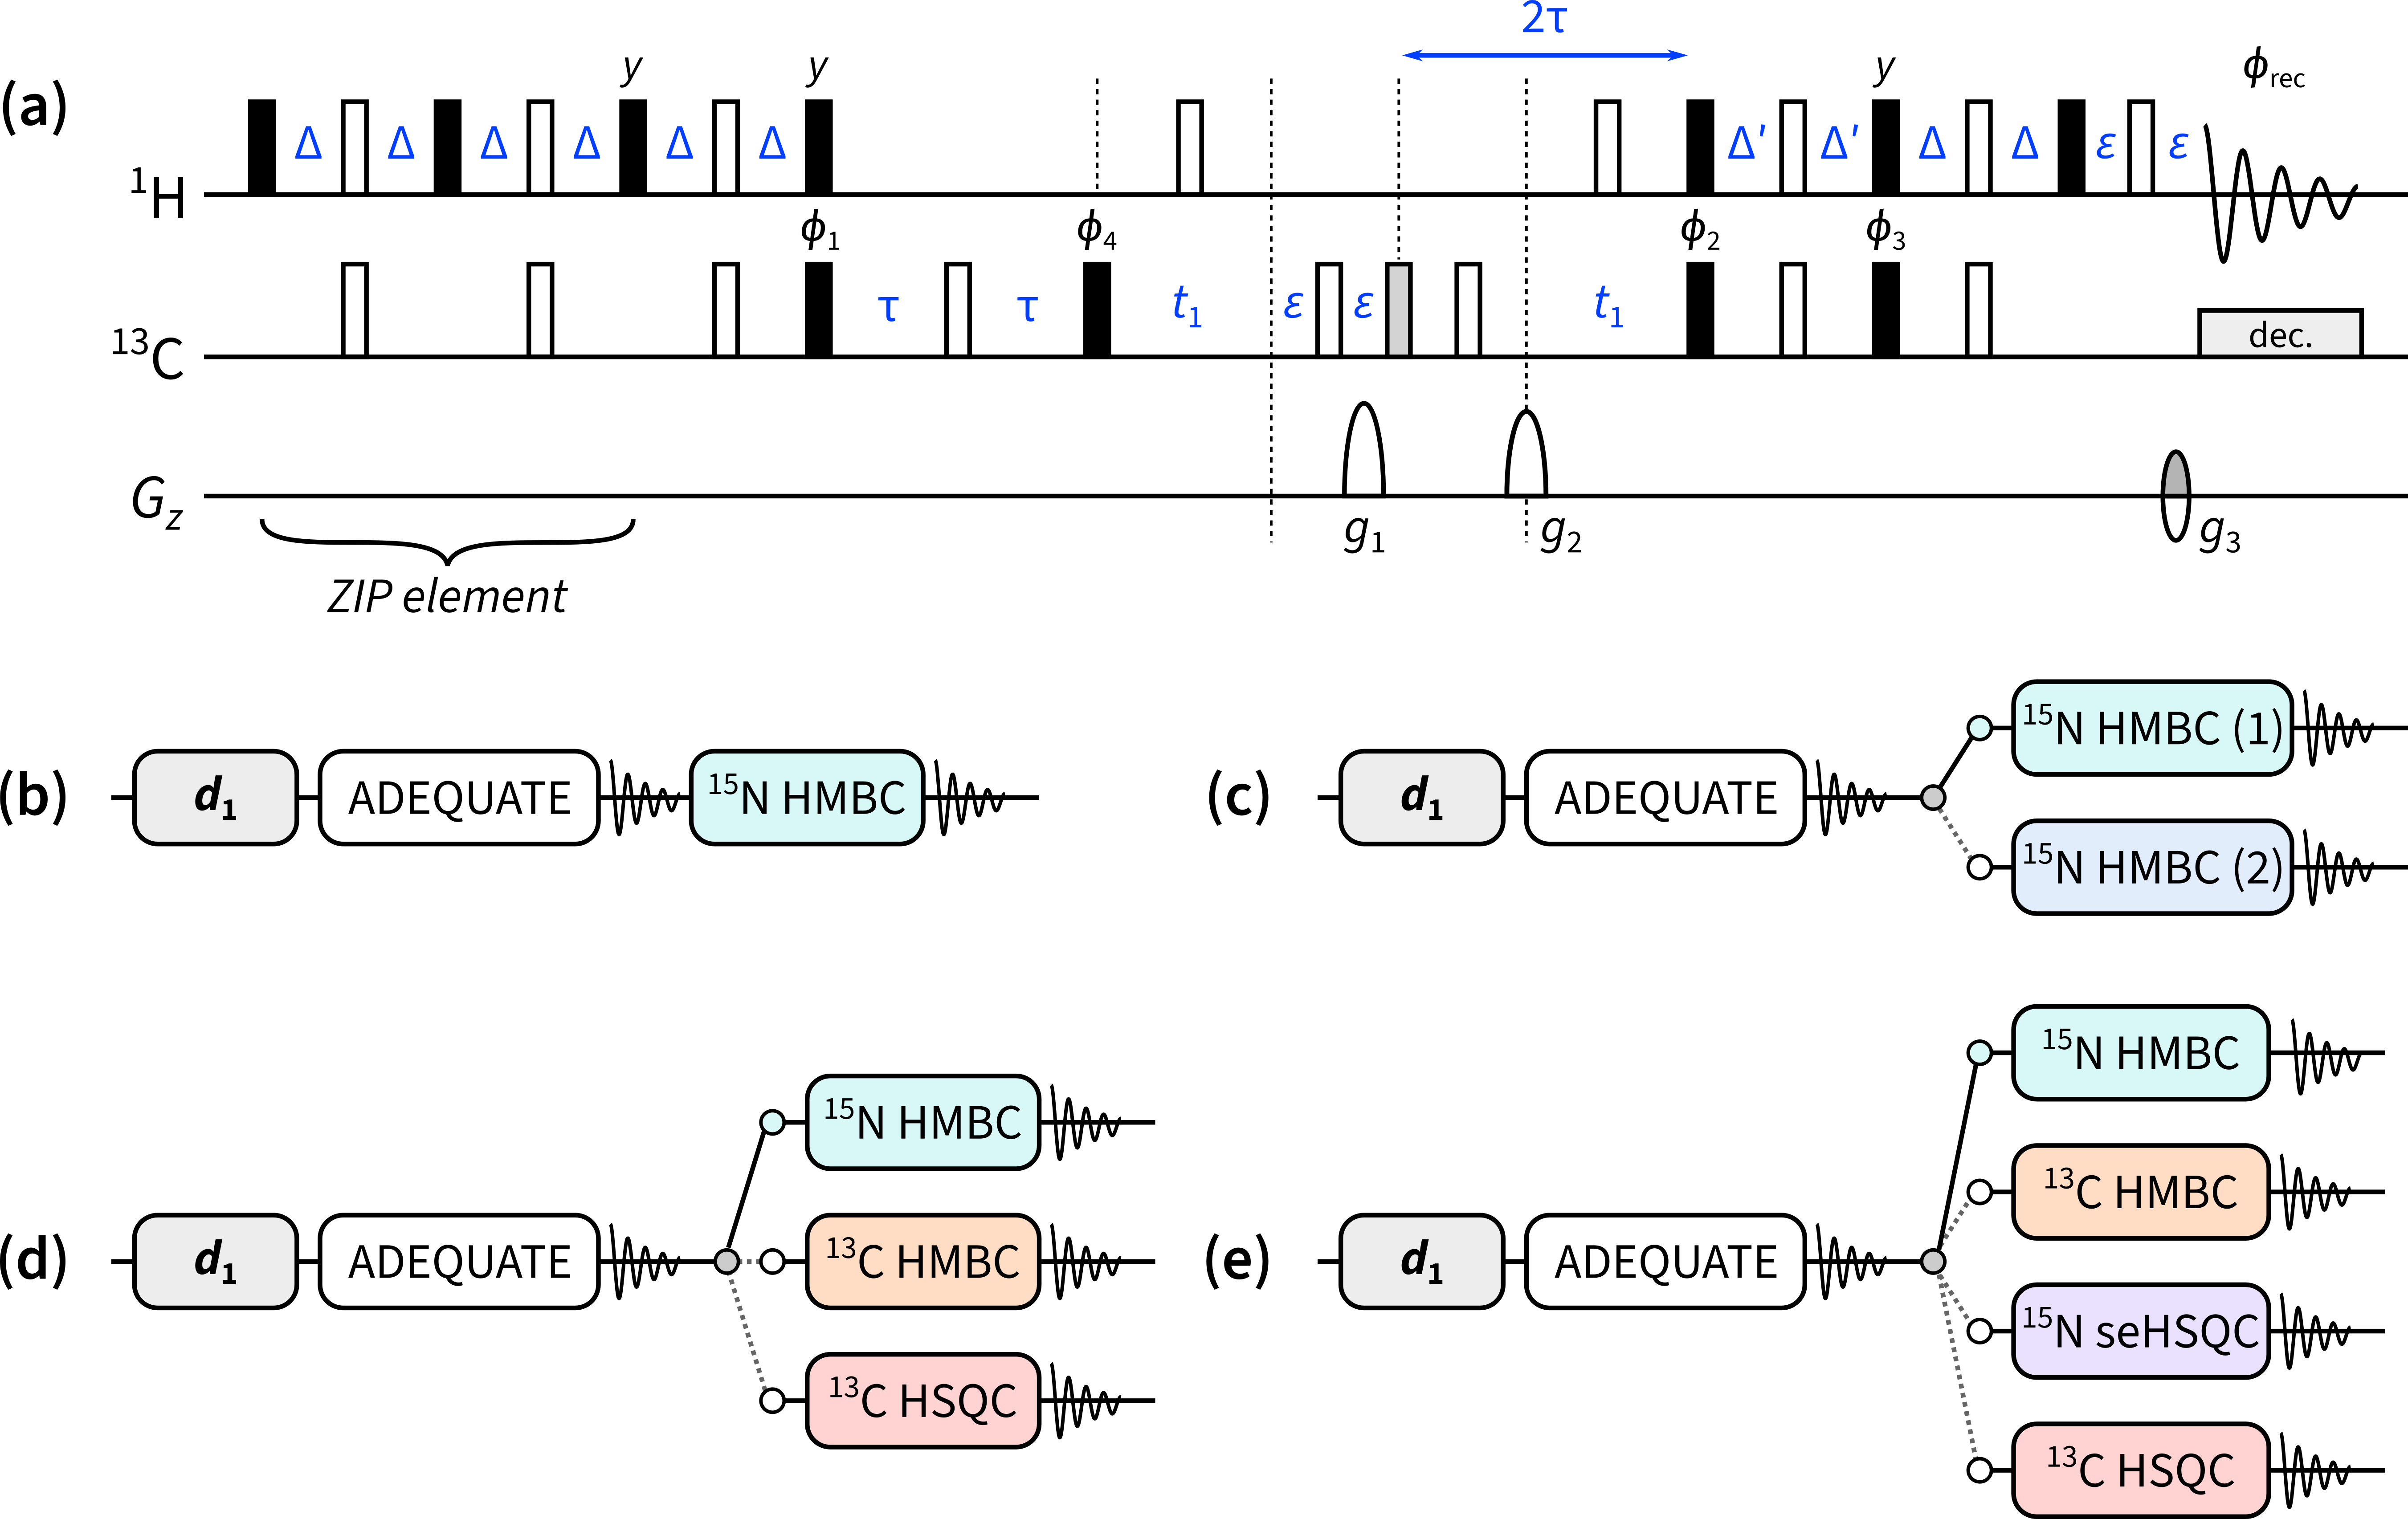
\includegraphics[]{sequences.png}%
    {\phantomsubcaption\label{fig:sequences_adequate}}
    {\phantomsubcaption\label{fig:sequences_ab}}
    {\phantomsubcaption\label{fig:sequences_abb}}
    {\phantomsubcaption\label{fig:sequences_abbs}}
    {\phantomsubcaption\label{fig:sequences_abbss}}
    \caption{
        Pulse sequences described in this work.
        \textbf{(\subref*{fig:sequences_adequate})} ZIP-1,1-ADEQUATE module.
        Filled and empty bars refer to \ang{90} and \ang{180} pulses respectively; the grey filled bar is a \ang{120} pulse for \carbon{} double-quantum to single-quantum coherence transfer\autocite{Mareci1982JMR}.
        Pulse and receiver phases are: $\phi_1 = x, -x$; $\phi_2 = 2\,(x), 2\,(-x)$; $\phi_3 = 2\,(y), 2\,(-y)$; $\phi_4 = 4\,(x), 4\,(-x)$; $\phi_\text{rec} = x, -x, -x, x, -x, x, x, -x$.
        Delays are set as follows: $\Delta = 1 / (4 \cdot \onejch)$, $\Delta' = 1 / (8 \cdot \onejch)$, and $\tau = 1 / (4 \cdot \onejcc)$. $\varepsilon$ is the minimum time required for a pulsed field gradient and the following recovery delay.
        Gradient amplitudes as a percentage of the maximum amplitude are: $g_1 = 78.5\%$, $g_2 = 77.6\%$, and $g_3 = -59\%$.
        Echo--antiecho selection is achieved by inverting the sign of $g_3$ as well as the pulse phase $\phi_3$.
        \textbf{(\subref*{fig:sequences_ab})} \abn{} supersequence.
        \textbf{(\subref*{fig:sequences_abb})} \abnbn{}, where the two \nitrogen{} HMBC experiments are optimised for two different values of $\njnh{}$.
        \textbf{(\subref*{fig:sequences_abbs})} \abnbs{}.
        \textbf{(\subref*{fig:sequences_abbss})} \abnbspns{}.
    }
    \label{fig:sequences}
\end{figure}

\section{NOAH-2 AB\texorpdfstring{$_{\ch{N}}$}{n}}

When designing NMR supersequences, it is generally a good rule of thumb to place the module with the lowest sensitivity first: this is because any incomplete preservation of magnetisation by earlier modules will lead to decreased sensitivity in later modules.
The 1,1-ADEQUATE module, which relies on neighbouring pairs of \carbon{} nuclei---occurring only in roughly 1 out of 8130 molecules---is therefore placed at the beginning of all the supersequences described here.

The ADEQUATE module (\cref{fig:sequences_adequate}) is designed to only use the magnetisation of protons directly bonded to \carbon{}, which we denote here as \magn{\ch{C}}.\autocite{Orts2018M,Yong2021JMR}
In order to maintain the sensitivity of later modules, it must return the magnetisation of all other protons (denoted as \magnnot{\ch{C}}) to the equilibrium $+z$ state.
This is accomplished by replacing the initial \ang{90} excitation pulse by the $zz$ isotope-selective pulse element (ZIP)\autocite{Hansen2021AC,Yong2021JMR}, which effects \angang{90}{-x} and \angang{90}{-y} rotations on \magn{\ch{C}} and \magnnot{\ch{C}} magnetisation respectively.
(Other isotope-specific elements such as BANGO\autocite{Sorensen1994BMR,Nagy2019CC,Nagy2021ACIE} may also be used here, with similar results generally being obtained.\autocite{Yong2021JMR})
The \nitrogen{} HMBC module of choice is a simple magnitude-mode version, with an optional first-order low-pass J-filter.
In the \abn{} supersequence (\cref{fig:sequences_ab}), this module simply consumes the remaining \magnnot{\ch{C}} magnetisation which was preserved by the ZIP-ADEQUATE module.

\begin{figure}[ht]
    \centering
    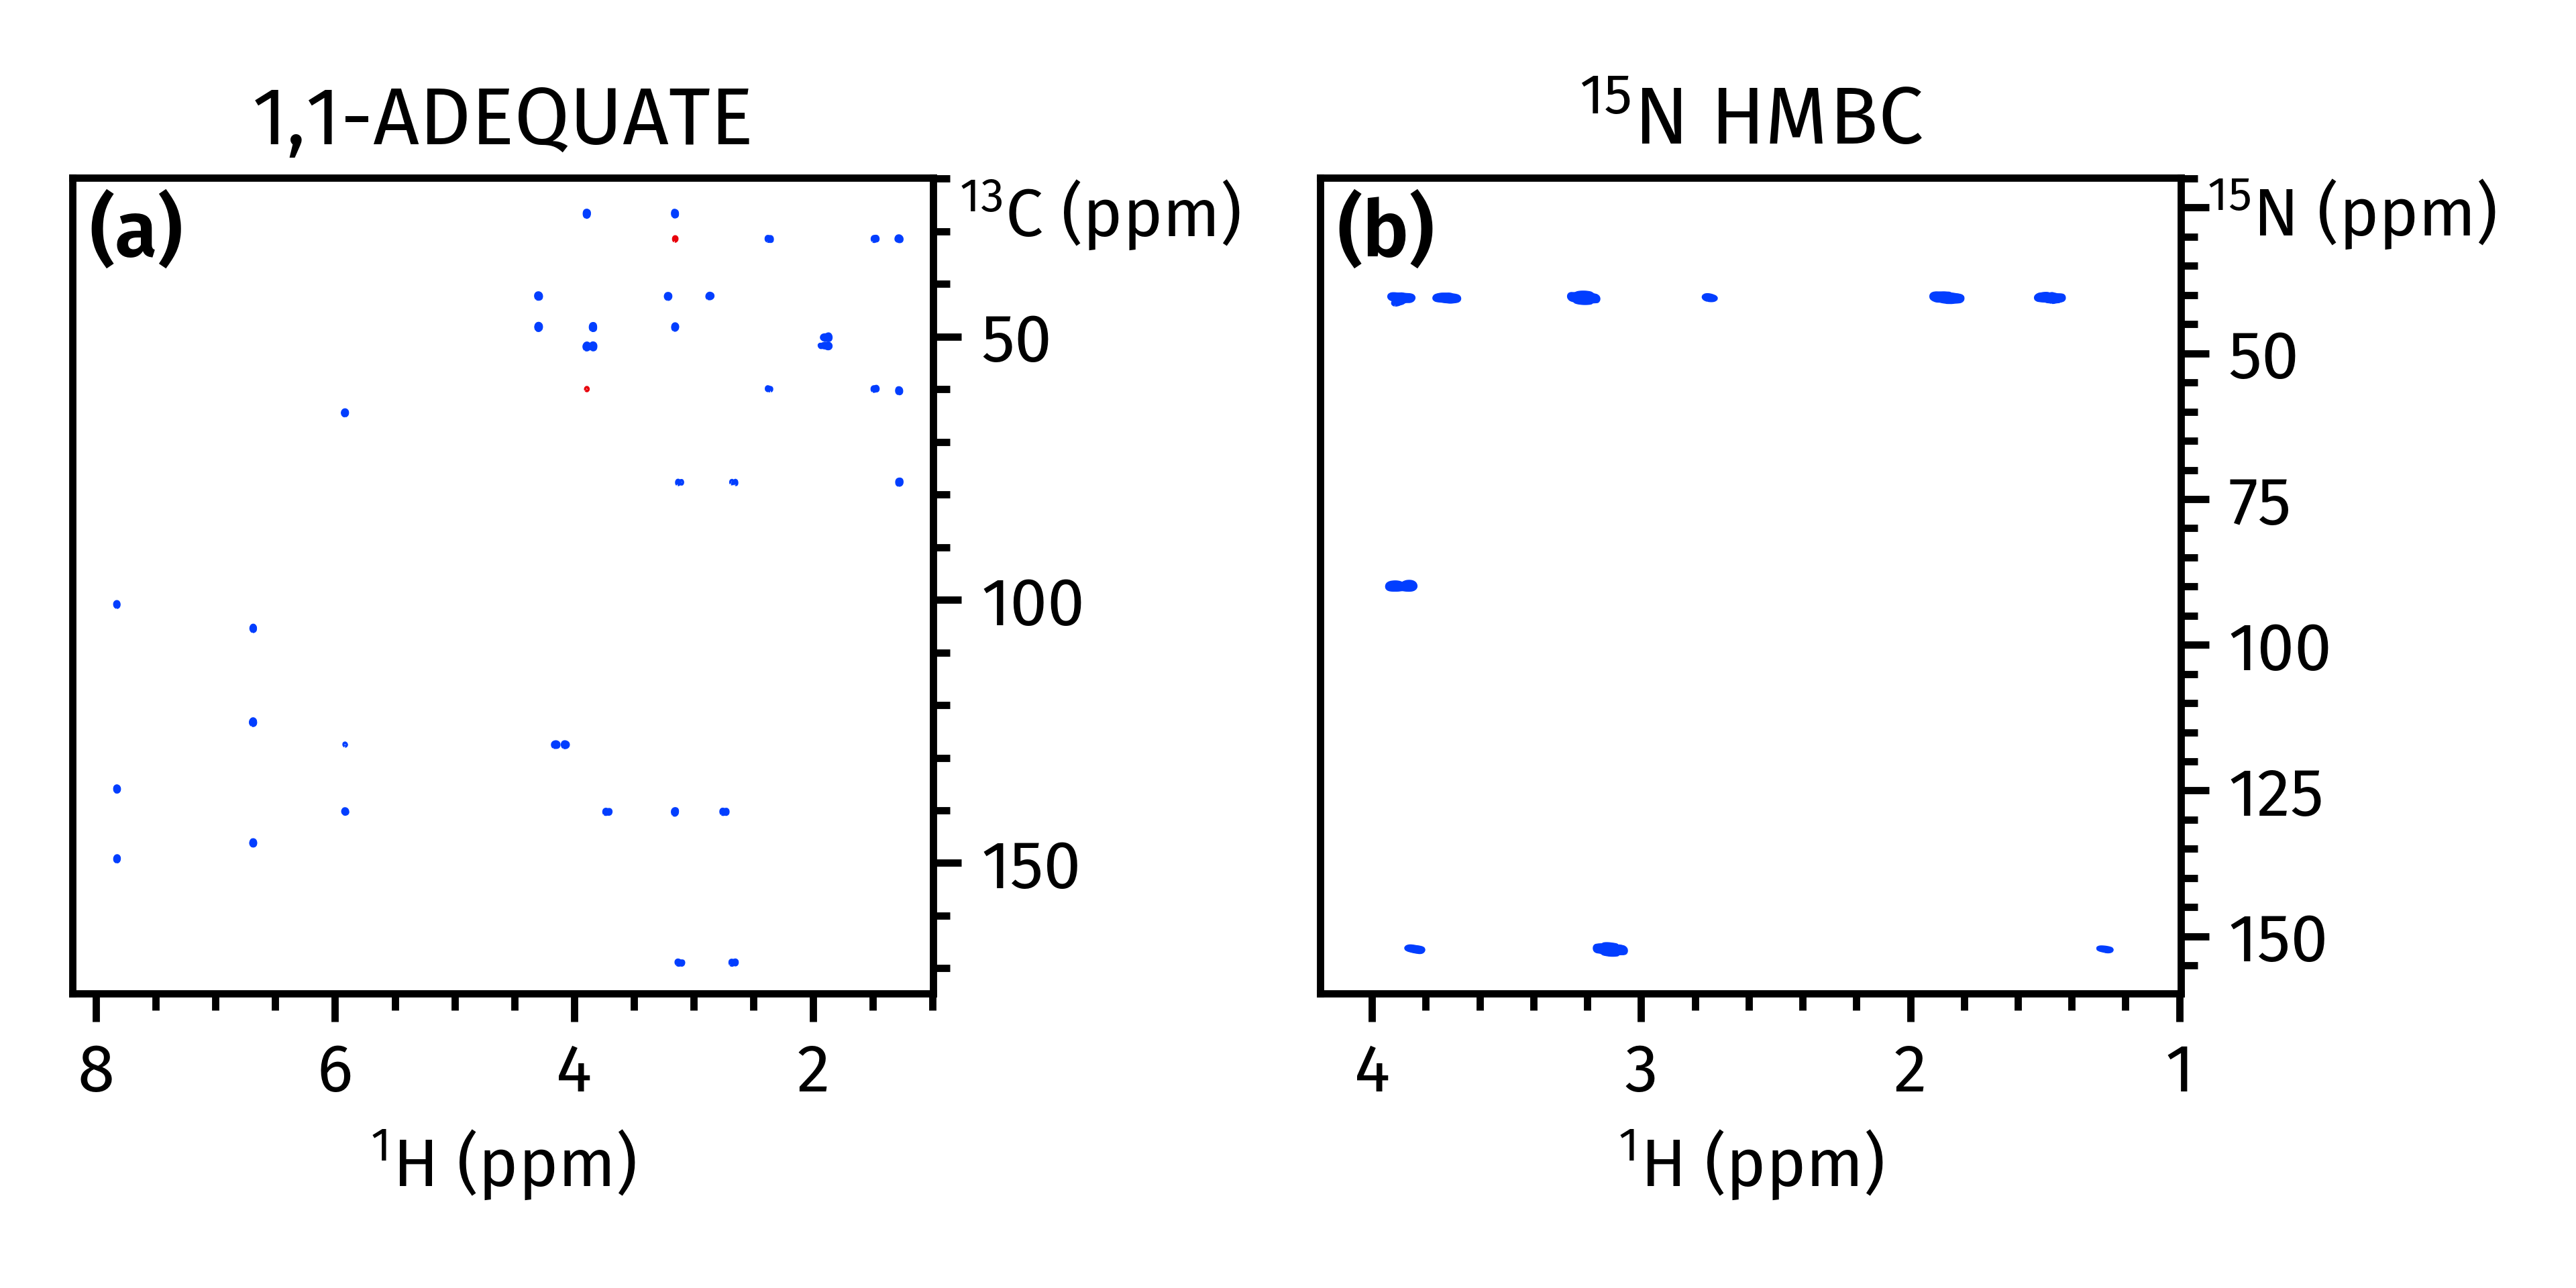
\includegraphics[]{ab.png}%
    {\phantomsubcaption\label{fig:ab_adeq}}
    {\phantomsubcaption\label{fig:ab_n_hmbc}}
    \caption{
        Spectra obtained from the \abn{} supersequence.
        \textbf{(\subref*{fig:ab_adeq})} 1,1-ADEQUATE.
        \textbf{(\subref*{fig:ab_n_hmbc})} \nitrogen{} HMBC.
        \brucine{} (see \cref{fig:samples_brucine} for structure).
    }
    \label{fig:ab}
\end{figure}


\section{NOAH-3 AB\texorpdfstring{$_{\ch{N}}$}{n}B\texorpdfstring{$_{\ch{N}}$}{n}}

Although this \abn{} sequence performs well on its own (\cref{fig:ab}), it suffers from the drawback that the \nitrogen{} HMBC is optimised for one specific value of $\njnh$.
In practice, $\njnh{}$ values range from \qtyrange{2}{16}{Hz}; in a single HMBC experiment, some correlations may therefore be lost due to J-coupling mismatch.

To circumvent this issue, a variety of accordion-type experiments\autociteset{accordion_hmbc} have been designed which decrement the J-evolution period in step with $t_1$, allowing a wider range of couplings to be sampled.
Alternatively, and perhaps more commonly, two (or more) separate HMBC experiments, optimised for different $\njnh$ values, can be recorded; the resulting spectra may be co-added to mimic an accordion-type HMBC if desired.
These separate HMBC modules cannot be recorded \textit{sequentially}, as they both draw on the same \magnnot{\ch{C}} magnetisation.
However, they can easily be executed in an \textit{interleaved} or parallel manner where, after the ADEQUATE module, the two HMBC experiments are alternately acquired.\autocite{Kupce2021JACSA}
In \cref{fig:sequences_abb}, this is illustrated by a `vertical' stacking of the two modules.
Thus, after each odd-numbered increment of the ADEQUATE, the first HMBC is acquired; and after each even-numbered increment, the second HMBC is acquired.
This means that both HMBC spectra have half the usual number of $t_1$ increments compared to the ADEQUATE, which is acceptable since the \nitrogen{} dimension is typically sparse and a high resolution is not required; furthermore, since the \nitrogen{} HMBC is more sensitive than the ADEQUATE, the reduced number of FIDs recorded per HMBC is practically inconsequential.
As can be seen in \cref{fig:abb}, the two HMBC spectra reveal different sets of correlations, allowing for more confident structural determination.

\begin{figure}[ht]
    \centering
    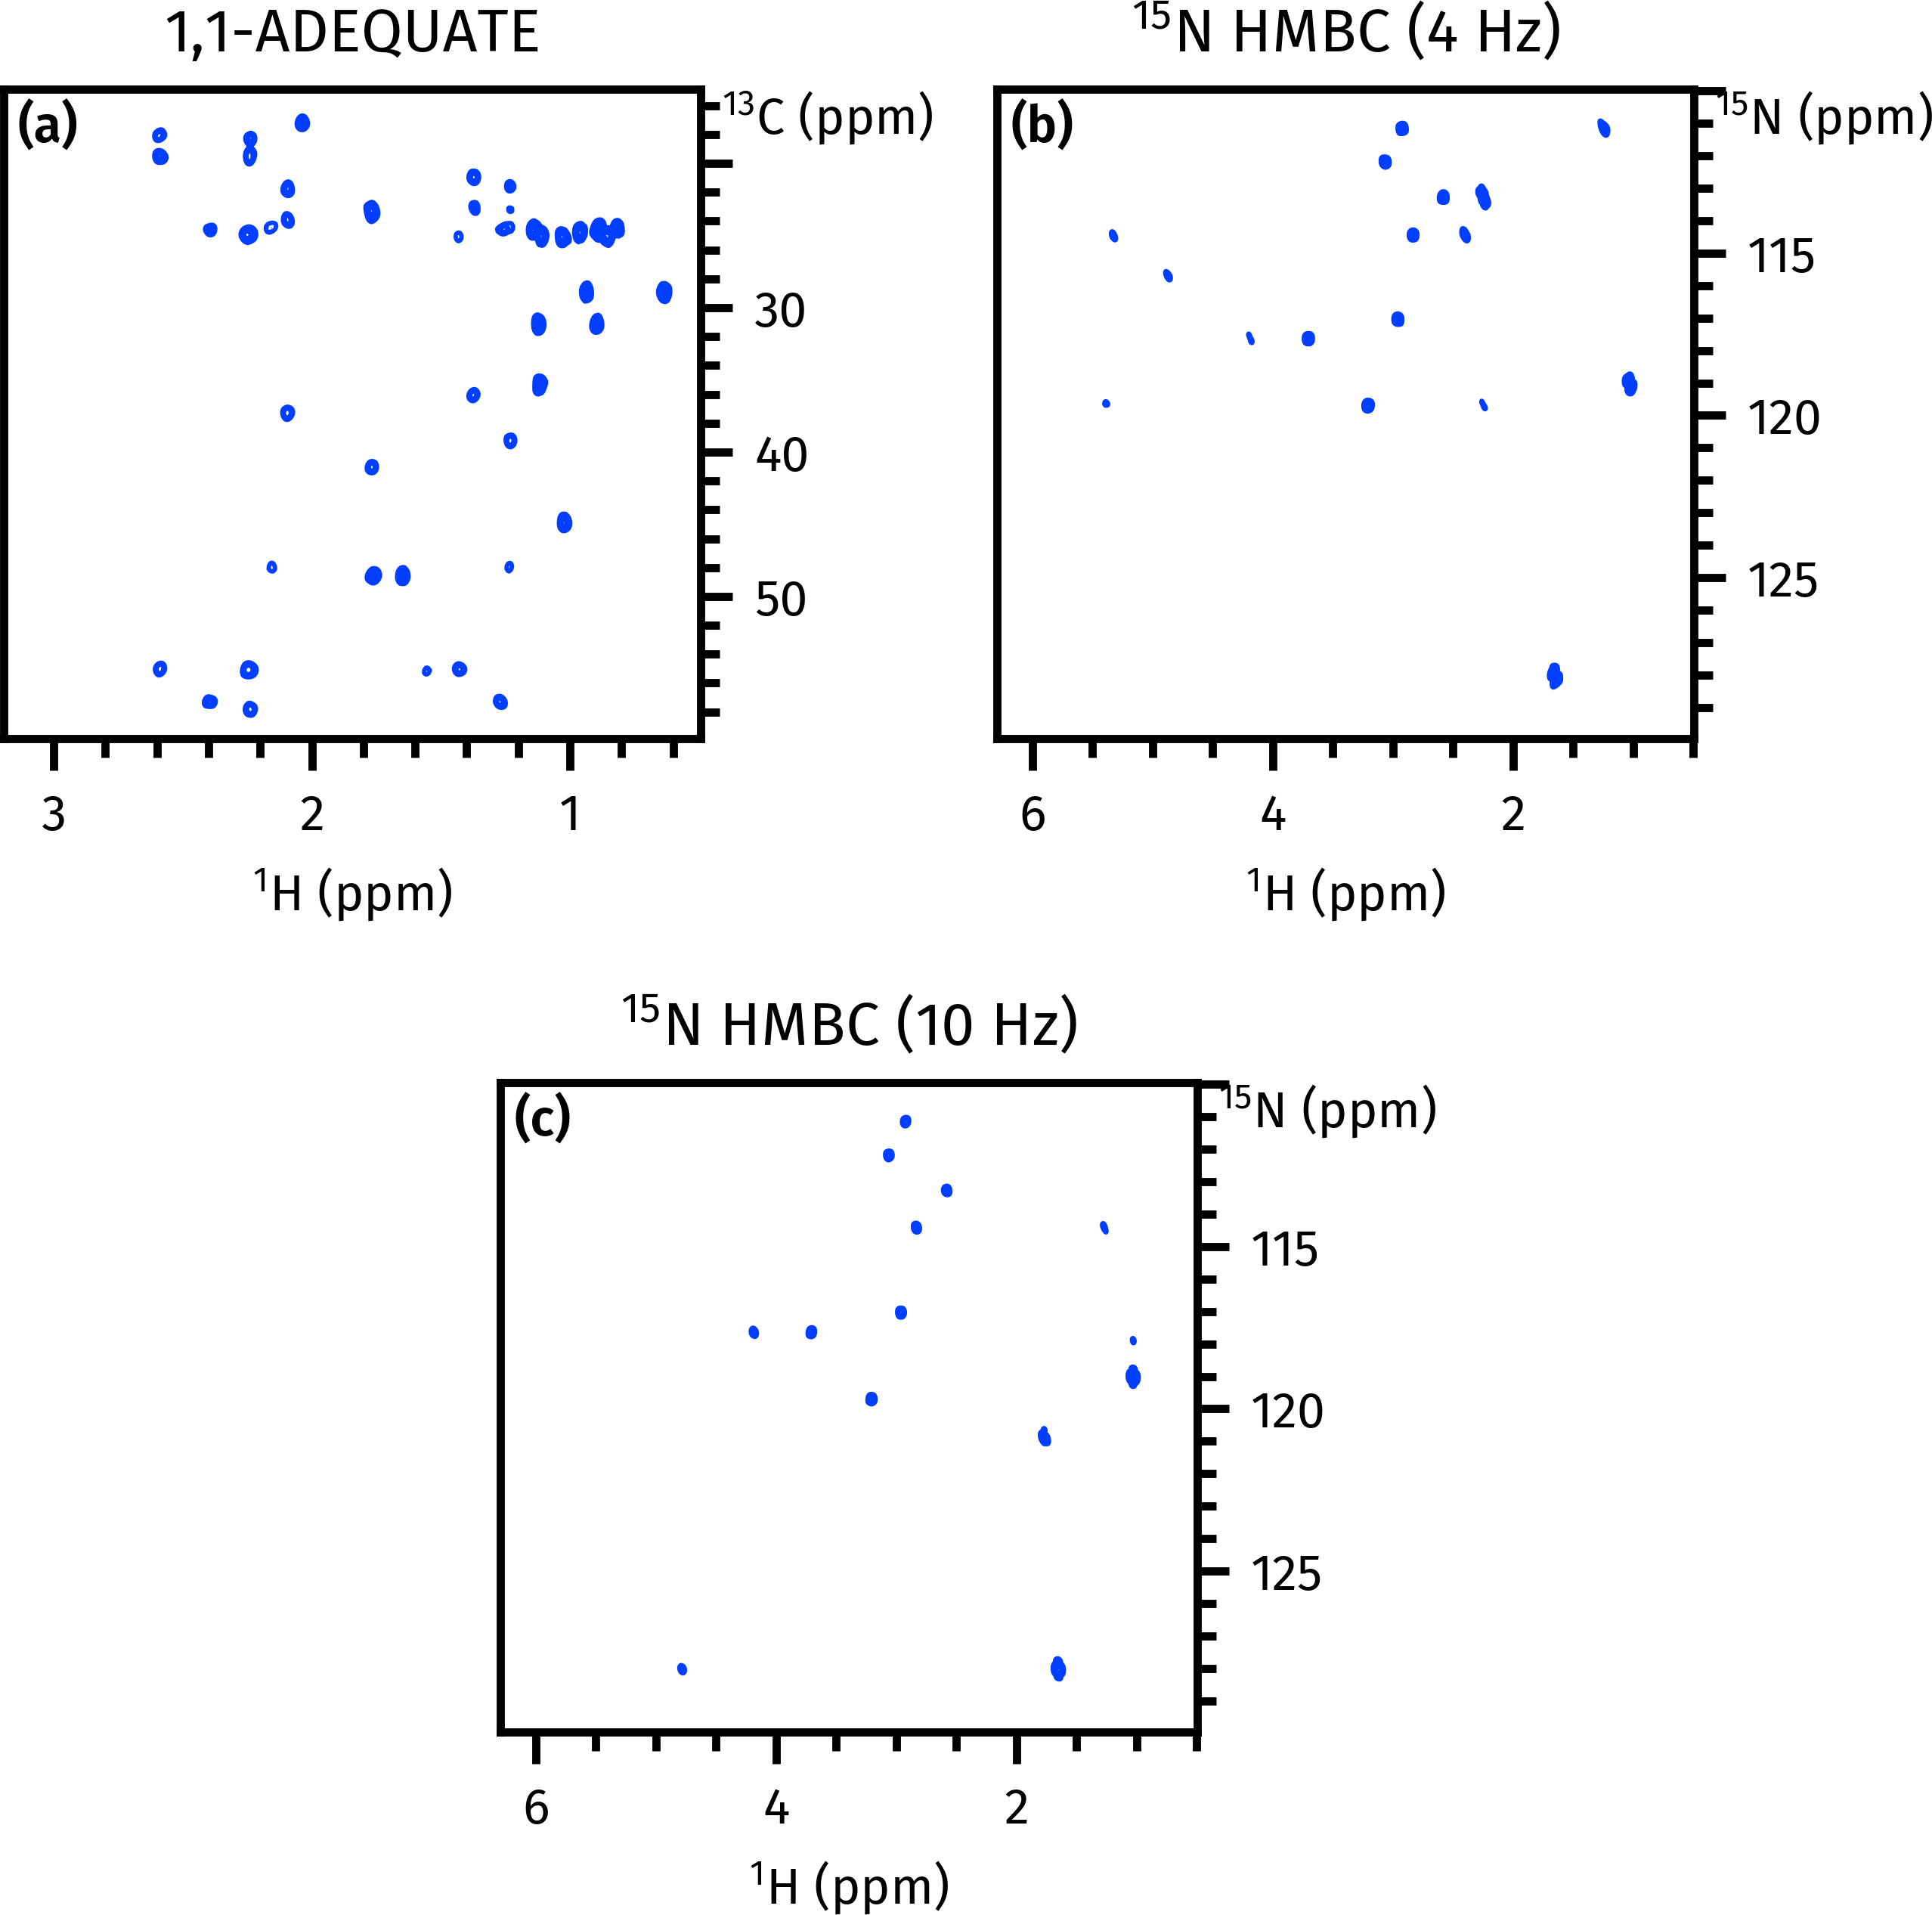
\includegraphics[]{abb.png}%
    {\phantomsubcaption\label{fig:abb_adeq}}
    {\phantomsubcaption\label{fig:abb_n_hmbc1}}
    {\phantomsubcaption\label{fig:abb_n_hmbc2}}
    \caption{
        Spectra obtained from the \abnbn{} supersequence.
        \textbf{(\subref*{fig:abb_adeq})} 1,1-ADEQUATE (256 $t_1$ increments).
        \textbf{(\subref*{fig:abb_n_hmbc1})} \nitrogen{} HMBC optimised for $\njnh = \SI{4}{Hz}$ (128 $t_1$ increments).
        \textbf{(\subref*{fig:abb_n_hmbc2})} \nitrogen{} HMBC optimised for $\njnh = \SI{10}{Hz}$ (128 $t_1$ increments).
        \cyclo{} (see \cref{fig:samples_cyclosporin} for structure).
    }
    \label{fig:abb}
\end{figure}

\section{NOAH-4 AB\texorpdfstring{$_{\ch{N}}$}{n}BS}

In the above \abnbn{} experiment and in previous work,\autocite{Kupce2021JACSA} we have shown how two alternating modules can be used to construct parallel supersequences.
This concept can naturally be further generalised in order to allow two or more different experiments to be acquired alternately as the second module in the supersequence.
These interleaved experiments can be arranged such that they each have lower resolution compared to the first module (as was done here), or such that they each have a fewer number of transients.
In principle, such an arrangement can be used for \textit{all} modules in a supersequence, not just the second module as is done here.
However, it is important to remember that earlier modules affect the amount of magnetisation passed on to the later modules; thus, interleaving later modules in a sequence usually leads to more robust supersequences with minimal discrepancies in data intensity or spectral quality.

In the \abnbs{} supersequence (\cref{fig:sequences_abbs}), the ADEQUATE module is followed by one of three choices: a \nitrogen{} HMBC, a \carbon{} HMBC (denoted \noah*{B}), or a \carbon{} HSQC (denoted \noah*{S}).
Because these three latter modules do not have the same intrinsic sensitivity, we balance this by allocating a different number of transients to each module.
In this specific example, each $t_1$ increment of the ADEQUATE collects a total of $8n$ transients (where $n$ is some positive integer); the \nitrogen{} HMBC $6n$ transients; and the \carbon{} HMBC and HSQC $n$ transients each.
The value of $n$ is chosen to ensure that all spectra have sufficient sensitivity; the spectra in \cref{fig:abbs} were acquired with $n = 2$.
Using the pulse programmes provided in the \SInf{}, the exact number of transients for each module can be customised via user-defined constants.
The exact implementation of these supersequences is described in detail in \cref{sec:pp_detail}.

\begin{figure}[ht]
    \centering
    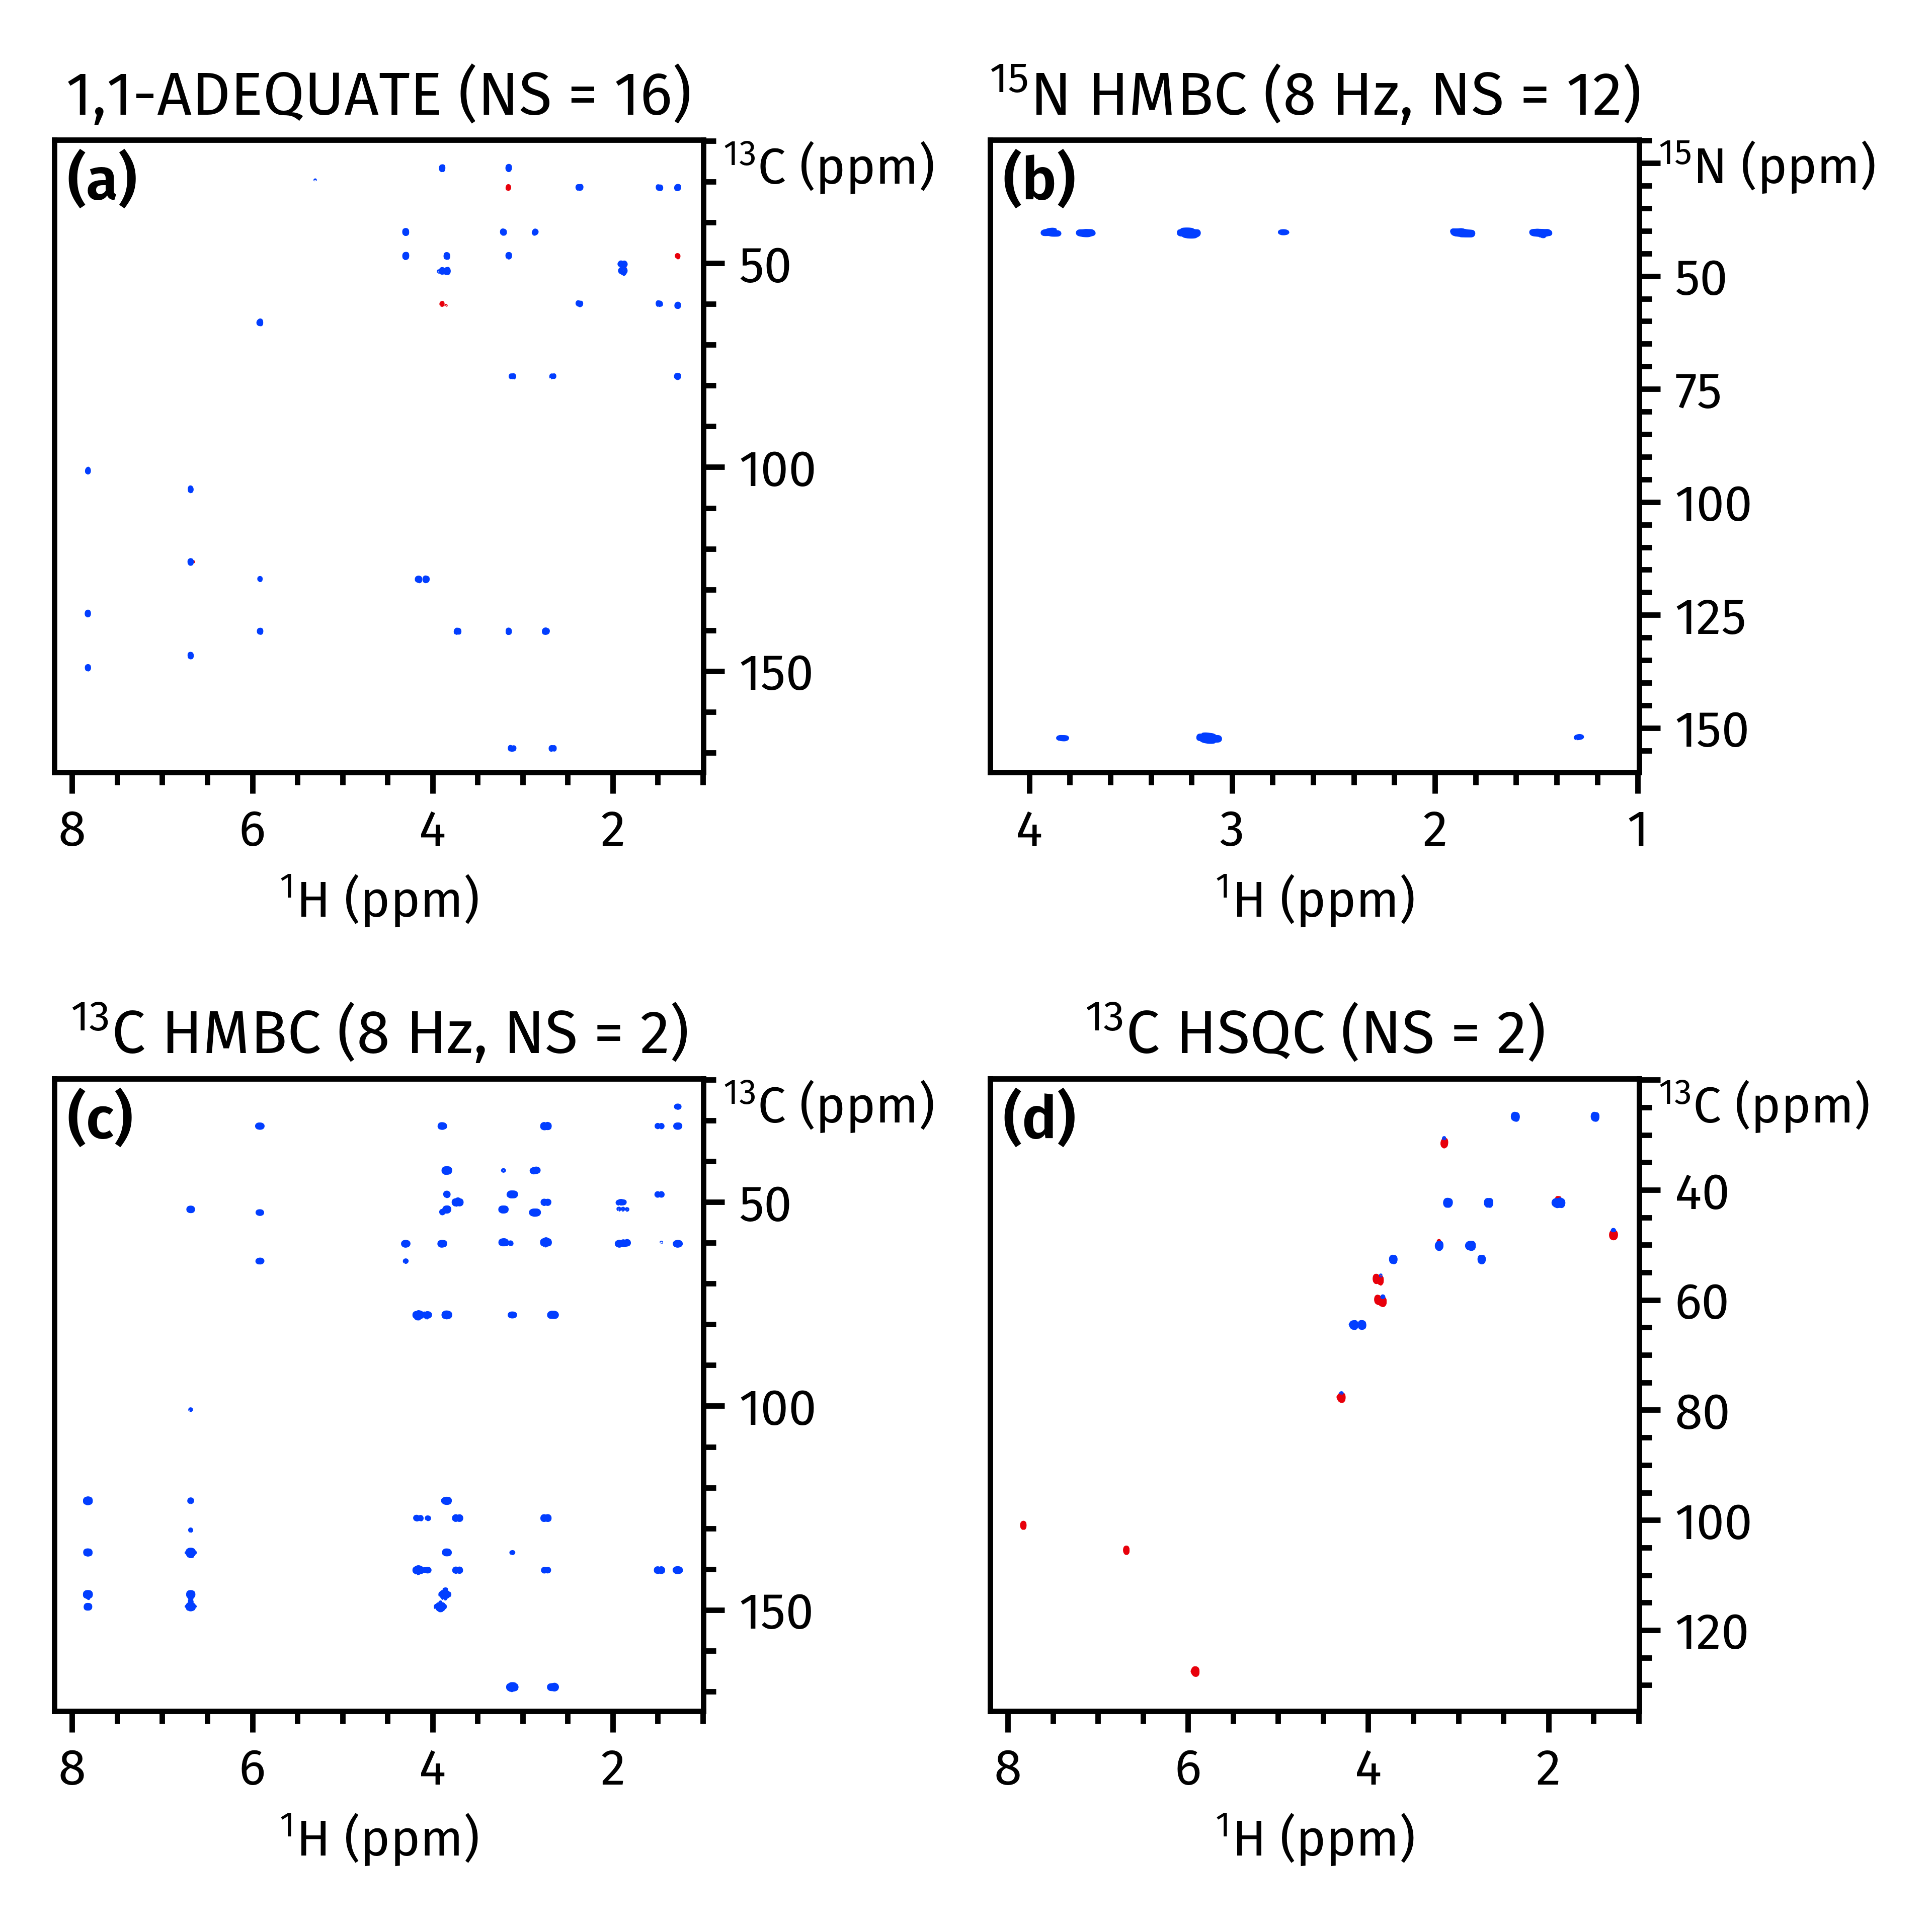
\includegraphics[]{abbs.png}%
    {\phantomsubcaption\label{fig:abbs_adeq}}
    {\phantomsubcaption\label{fig:abbs_n_hmbc}}
    {\phantomsubcaption\label{fig:abbs_c_hmbc}}
    {\phantomsubcaption\label{fig:abbs_c_hsqc}}
    \caption{
        Spectra obtained from the \abnbs{} supersequence.
        All modules were recorded with 256 $t_1$ increments.
        \textbf{(\subref*{fig:abbs_adeq})} 1,1-ADEQUATE (16 transients).
        \textbf{(\subref*{fig:abbs_n_hmbc})} \nitrogen{} HMBC (12 transients).
        \textbf{(\subref*{fig:abbs_c_hmbc})} \carbon{} HMBC (2 transients).
        \textbf{(\subref*{fig:abbs_c_hsqc})} \carbon{} HSQC (2 transients).
        \brucine{}.
    }
    \label{fig:abbs}
\end{figure}

The acquisition of the \abnbs{} spectra in \cref{fig:abbs} took 124 minutes; in contrast, normal acquisition of all four experiments (with the equivalent number of transients per module) required a total of 223 minutes.
As the ADEQUATE is placed first in the supersequence, its sensitivity is almost identical to that of a standalone ADEQUATE; the inclusion of the ZIP element causes only an approximate 5\% loss.
The \nitrogen{} and \carbon{} HMBC spectra experience small losses (16--29\%) in sensitivity, due to imperfect magnetisation retention by the ADEQUATE module.
This is, however, outweighed by the almost twofold time savings provided by concatenation of the modules: if the NOAH supersequence were acquired for as long as the standalone experiments were, the \nitrogen{} HMBC spectra would have almost the same SNR, and the \carbon{} HMBC from the NOAH would in fact have a 12\% improvement in SNR.
Due to the reuse of \magn{\ch{C}} magnetisation, the HSQC module only retains 29\% of its original sensitivity.
However, as the HSQC is still two orders of magnitude more sensitive than the ADEQUATE, this decrease is readily tolerated; if necessary, the sensitivity-enhanced HSQC module\autocite{Hansen2021AC,Yong2021JMR} may also be used in its place.

While this combination of modules proves to be particularly elegant in that it furnishes virtually all heteronuclear correlations needed for structural assignment of nitrogen-containing organic molecules, it is by no means the only valid one.
The principle of interleaved modules can be used to incorporate almost any experiment that may be required: as an example, spectra from a \abnns{} experiment (N = NOESY, replacing the \carbon{} HMBC) are shown in \cref{fig:abns}.

\section{NOAH-5 AB\texorpdfstring{$_{\ch{N}}$}{n}BS\texorpdfstring{$^+_{\ch{N}}$}{+n}S}

As a final example, we add a further \nitrogen{} seHSQC module to the above sequence.
The \nitrogen{} seHSQC uses only \magn{\ch{N}} magnetisation (i.e.\ protons directly bonded to \nitrogen{}), which is separate from all other modules introduced so far.
Thus, in principle, it can simply be added \textit{linearly} as a third sequential module to the supersequence: such an arrangement would maximise its sensitivity as the \nitrogen{} seHSQC data are collected on every scan in the supersequence.
Such an arrangement would, however, compromise the performance of the other modules, as they must then be modified to preserve the requisite \magn{\ch{N}} magnetisation: for example, the HMBC modules would need to be modified to include the $zz$-filter\autocite{Kupce2018CC,Kupce2019JMR}, which leads to further sensitivity losses.
Instead of this, the \nitrogen{} seHSQC can most efficiently be implemented in a `vertical', interleaved manner, by simply reducing the number of transients for the \nitrogen{} HMBC by $n$ and diverting these towards the \nitrogen{} seHSQC.
This means that the second slot in the supersequence now alternates between four different experiments, as shown in \cref{fig:sequences_abbss}.
This example especially illustrates how the use of interleaved \textit{and} sequential acquisition leads to much greater flexibility in supersequence design, especially when considering the relative sensitivities of different modules.

The five spectra obtained from this sequence are shown in \cref{fig:abbss}.
Collectively, this supersequence provides virtually all heteronuclear correlation data required for structural elucidation or assignment.
These can further be processed using covariance techniques\autociteset{indirect-covariance} to yield double-heteronuclear correlation spectra (\cref{sec:si_covariance}).
This supersequence is similar in spirit to the PANACEA experiment\autociteset{panacea}, but yields greater sensitivity as it uses equilibrium \proton{} magnetisation rather than the low-magnetogyric ratio \carbon{} and \nitrogen{} nuclei, and does not require multiple-receiver hardware.\autocite{Kupce2021PNMRS,Kupce2021NRMP}
Of course, the ADEQUATE experiment may not be necessary for every novel compound encountered.
However, in cases where it \textit{is} needed, the supersequences described here demonstrate that other valuable heteronuclear spectra can also be acquired together with the ADEQUATE in a manner which yields significant time savings and sensitivity per unit time improvements.

\section{Conclusion(ish)}

In conclusion, we have demonstrated here how low-sensitivity experiments, such as 1,1-ADEQUATE and \nitrogen{} HMBC, may be optimally combined in NMR supersequences, leading to substantial reductions in experiment time.
Through a generalisation of our previous concept of parallel supersequences, further high-sensitivity  modules may be added to the supersequence both `horizontally' and `vertically', corresponding respectively to sequential and interleaved/parallel acquisition.
The spectra thus obtained provide the chemist with far more powerful tools for the characterisation of complex molecules, especially in cases where existing (sequential) NOAH supersequences do not provide sufficient information for unambiguous assignment.
a notable example of this is proton-sparse nitrogen heterocycles, which are commonly found in pharmaceuticals.
The pulse programmes and processing scripts used in this work can be obtained via the Bruker User Library or GitHub; links are provided in Section S2 of the \textit{Supplementary Information}.


\section*{Acknowledgements}

We thank Dr Mohammadali Foroozandeh (University of Oxford) for helpful discussions.
\meshort{}\ thanks the Clarendon Fund (University of Oxford) and the EPSRC Centre for Doctoral Training in Synthesis for Biology and Medicine (EP/L015838/1) for a studentship, generously supported by AstraZeneca, Diamond Light Source, Defence Science and Technology Laboratory, Evotec, GlaxoSmithKline, Janssen, Novartis, Pfizer, Syngenta, Takeda, UCB, and Vertex.

% Fakesection Bibliography
\AtNextBibliography{\small}
\printbibliography{}
\end{refsection}


% Fakesection ================= SI ==================

\clearpage
\begin{refsection}
\newcommand{\sectionbreak}{\clearpage}
\renewcommand*{\thefigure}{S\arabic{figure}}
\renewcommand*{\thesection}{S\arabic{section}}
\renewcommand*{\thetable}{S\arabic{table}}
\renewcommand*{\thepage}{S\arabic{page}}
\setcounter{page}{1}
\setcounter{figure}{0}
\setcounter{section}{0}
\setcounter{table}{0}
\onehalfspacing

\hspace{0pt}
\vfill
\begin{center}
    \huge
    Supporting Information

    \vspace{0.3cm}

    \textit{for}

    \vspace{0.3cm}

    \articletitle{}

    \vspace{0.6cm}

    \Large \me{},\textsuperscript{1} \eriks{},\textsuperscript{2} \tim{}\textsuperscript{1,\texttt{*}}

    \vspace{0.6cm}

    \large \textsuperscript{1} \textit{\crl{}}

    \textsuperscript{2} \textit{\brukeruk{}}

    \textsuperscript{\texttt{*}} \texttt{tim.claridge@chem.ox.ac.uk}

\end{center}
\vfill

\newpage
\section*{Contents}

\startcontents[si]
\printcontents[si]{ }{1}{}
\vfill
\hspace{0pt}
\newpage

\section{Pulse programme description}
\label{sec:pp_detail}

This section presents a more detailed description of how the pulse programme works; this information is important to anybody seeking to use the pulse programmes given here (or anybody writing similar `interleaved' experiments).
We use the \abnbs{} experiment as an example here.
In this experiment, the second module alternates between the \nitrogen{} HMBC (\noah*{Bn}), \carbon{} HMBC (\noah*{B}), and \carbon{} HSQC (\noah*{S}); the pulse programme is set up such that these three modules have fewer transients than the ADEQUATE (\noah*{A}).
For every 8 transients of the ADEQUATE, 6, 1, and 1 transient(s) are recorded for the \noah*{Bn}, \noah*{B}, and \noah*{S} modules respectively.

An excerpt of the pulse programme is shown here and explained on the next page:

{\singlespacing
\begin{tcbminted}{bruker}
  "l3 = 0"      ; initialise loop counter
  "cnst51 = 8"  ; number of transients for ADEQUATE
  "cnst52 = 6"  ; number of transients for 15N HMBC
  "cnst53 = 1"  ; number of transients for 13C HMBC
  ; HSQC doesn't need a separate counter; it's just cnst51-cnst52-cnst53

2 d1

  ; run ADEQUATE
  goscnp ph30   ; record ADEQUATE FID

  if "l3 % cnst51 < cnst52" {
    ; transients 1 through 6: run 15N HMBC
    go=2 ph31
  }

  else {
  if "l3 % cnst51 < cnst52 + cnst53" {
    ; transient 7: run 13C HMBC
    go=2 ph31
  }

  else {
    ; transient 8: run 13C HSQC
    go=2 ph31   ; 'go' loops back to the label '2' a total of NS times
  }
  }

  1m iu3   ; increment loop counter
  if "l3 % cnst51 == 0" {
      ; increment t1 here
  }
  lo to 2 times x   ; see main text for description of x
\end{tcbminted}
}

Generally, interleaving is performed using modular arithmetic.
A loop counter (\texttt{L3}) is used in order to keep track of how many transients have been recorded so far, and the value of this counter \textit{modulo} 8 is used in order to determine which module to run in the second slot.
Note that this is independent of the \texttt{NS} parameter in TopSpin.
So, each $t_1$ increment of the ADEQUATE module is actually recorded $8 \times \texttt{NS}$ times.

Of course, the values of \texttt{cnst51}, \texttt{cnst52}, and \texttt{cnst53} are not hardcoded as in the example above.
By changing these numbers, the user can control the number of transients allocated to each module.
In total, each $t_1$ increment of the ADEQUATE module is acquired \texttt{cnst51} $\times$ \texttt{NS} times; the \nitrogen{} HMBC is acquired $\texttt{cnst52} \times \texttt{NS}$ times; and so on.
(For the final module (HSQC), there is no need to define an analogous \texttt{cnst54} because it simply `uses up' all the remaining transients; thus, the HSQC is acquired a total of $(\texttt{cnst51} - \texttt{cnst52} - \texttt{cnst53}) \times \texttt{NS}$ times.)

Finally, $t_1$ is only incremented if we have completed a full cycle of 8 runs through the loop.
Again, this is checked using modular arithmetic; every 8 loop iterations, \texttt{l3} will be a multiple of \texttt{cnst51}.
The value of $x$ in the last line corresponds to the total number of loop iterations which need to be made; thus, this value is equal to 8 times the number of desired $t_1$ increments.

\begin{figure}[!ht]
    \centering
    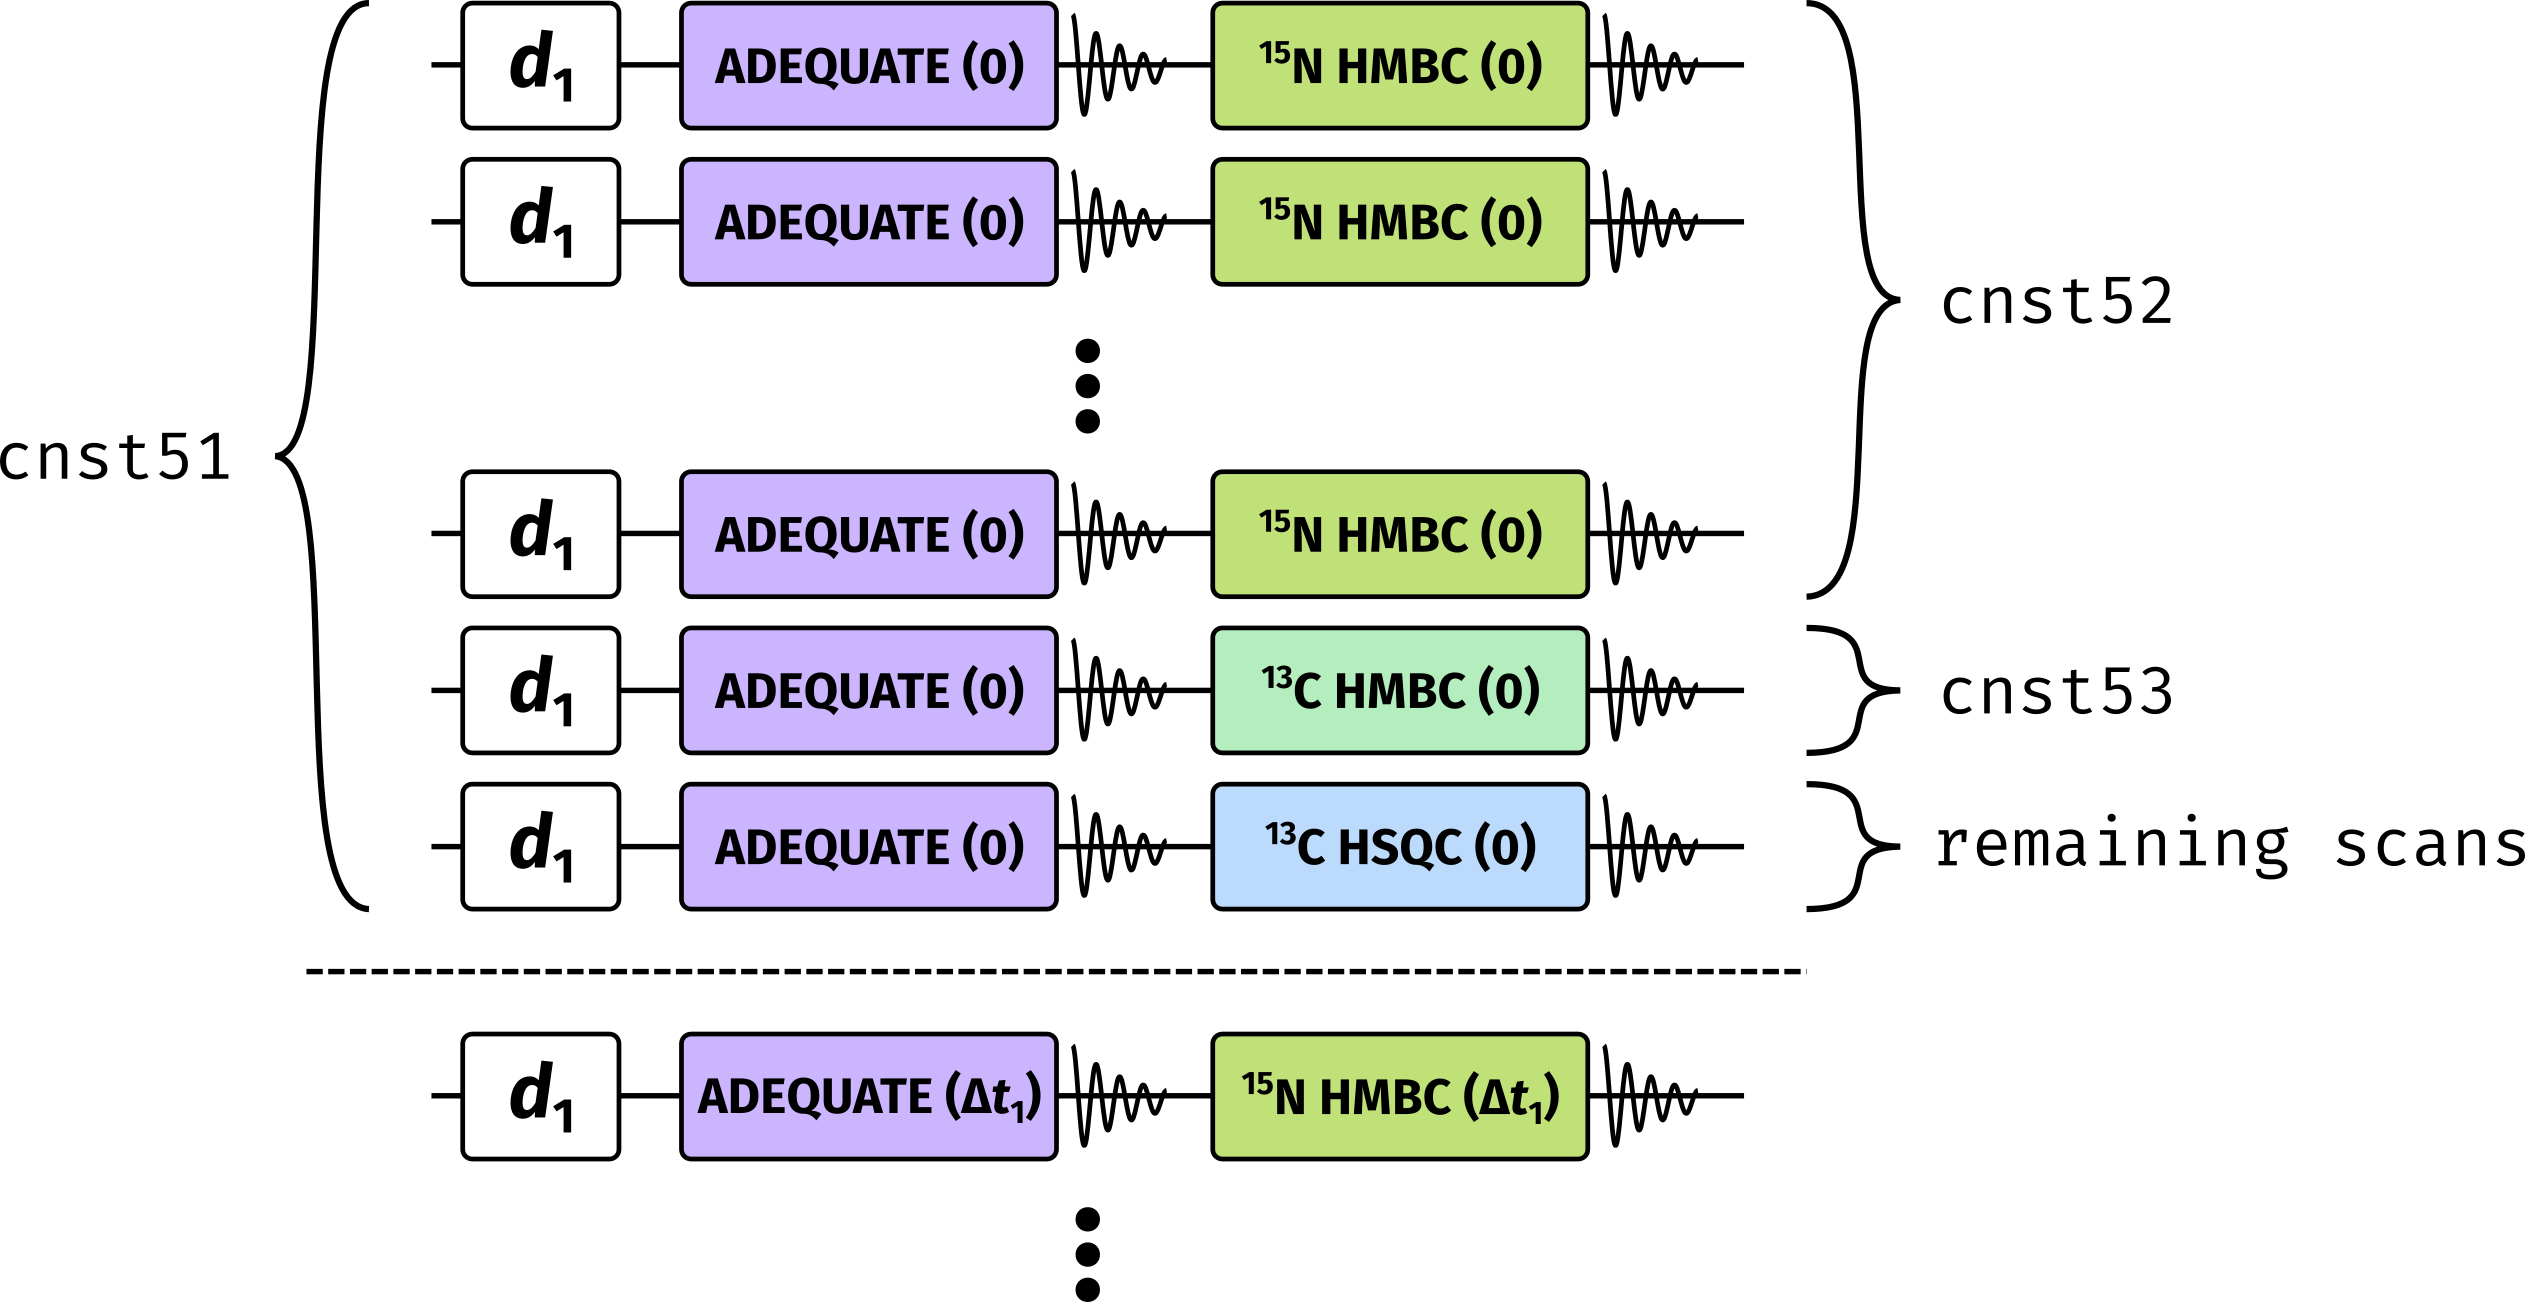
\includegraphics[scale=1.2]{figures/abbs_pp.png}%
    \caption[]{
        Diagram illustrating the practical implementation of the \abnbs{} supersequence.
        Numbers in parentheses refer to the value of $t_1$; the first increment is recorded with $t_1 = 0$ for all modules.
        $d_1$ represents a recovery delay.
        Each row is repeated \texttt{NS} times, during which phase cycling is performed; however, no phase cycling is performed \textit{between} rows, even those which are identical (e.g.\ the first two rows).
        Since each row only consists of two horizontally concatenated modules, the \texttt{NBL} parameter is to be still set to 2.
        The red arrow indicates where DIPSI-2 mixing is inserted: this is discussed in \cref{sec:si_dipsi}.
    }
    \label{fig:abbs_pp}
\end{figure}

It is worth pointing out at this point that, because of the way TopSpin increments pulse phase pointers, \textit{phase cycling} (as defined by the phase tables in the pulse programme) is only carried out \texttt{NS} times.
That is, although the ADEQUATE module is recorded \texttt{cnst51} $\times$ \texttt{NS} times, only a \texttt{NS}-step phase cycle is being used.
With modern gradient-based coherence selection techniques, this does not have a substantial impact on the data quality.
(For example, the data in \cref{fig:abbs} were recorded with \texttt{NS=2} and are perfectly serviceable.)
Nevertheless, it is always a good idea to make \texttt{NS} as large as possible, and always at least 2 to ensure suppression of axial peaks.
As a concrete illustration, the two parameter sets below yield the same signal-to-noise for all modules, but parameter set 2 will have a longer (and presumably better) 4-step phase cycle.

\begin{table}[H]
    \centering
    \begin{tabular}{ccc}
        \toprule
         & Parameter set 1, \texttt{NS=2} & Parameter set 2, \texttt{NS=4} \\
        \midrule
        \texttt{cnst51} & 12 & 6 \\
        \texttt{cnst52} & 8  & 4 \\
        \texttt{cnst53} & 2  & 1 \\
        $\texttt{cnst51} - \texttt{cnst52} - \texttt{cnst53}$ & 2  & 1 \\
        \bottomrule
    \end{tabular}
\end{table}

The parameter \texttt{NBL} should still be set to 2 for all of the supersequences shown in this work.
The \texttt{NBL} parameter corresponds to the number of \textit{sequentially} concatenated modules, which in all cases is only 2; the parallel modules play no role here.
The value of \texttt{TD1} should then be set to $\texttt{cnst51} \times \texttt{NBL} \times N_1$, where $N_1$ is the desired number of $t_1$ increments (i.e.\ \texttt{TD1} in a `traditional' 2D experiment).

Finally, it should be noted that the \texttt{if}/\texttt{else} conditionals are evaluated only at runtime by the spectrometer.
TopSpin does not calculate ahead of time when each interleaved module is run.
This means that the TopSpin \texttt{expt} command (which shows the expected experimental duration) can yield (very slightly) inaccurate results.

\section{Pulse programme and processing script availability}

The pulse programmes used in this work, along with all requisite processing scripts, can be downloaded from the Bruker User Library at \url{https://www.bruker.com/protected/en/services/bruker-user-library.html}, or equivalently, from GitHub at \url{https://github.com/yongrenjie/abbs-paper/releases/tag/data}.
The zip archive contains further instructions on setting up the pulse programmes.

\clearpage
\section{\texorpdfstring{\abnns{}}{NOAH-4 A(Bn/N/S)} experiment}

Since the \proton{}--\proton{} NOESY uses the same \magnnot{\ch{C}} magnetisation as \carbon{} HMBC so can be directly substituted in its place, leading to a \abnns{} supersequence (\cref{fig:abns}).
This not only provides a wealth of through-bond correlations which aid in eludicating molecular constitution, but also furnishes through-space correlations for the determination of configuration or conformation.
Depending on the molecular size and spectrometer frequency, the NOESY module may easily be replaced with a ROESY.

\begin{figure}[!ht]
    \centering
    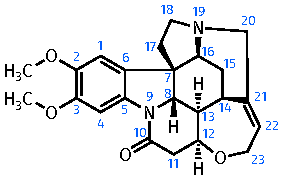
\includegraphics[]{brucine.pdf}%
    \caption[Structure of brucine]{
        Structure of brucine.
    }
    \label{fig:samples_brucine}
\end{figure}

\clearpage 
\begin{figure}[htb]
    \begin{subfigure}[b]{\textwidth}
        \centering
        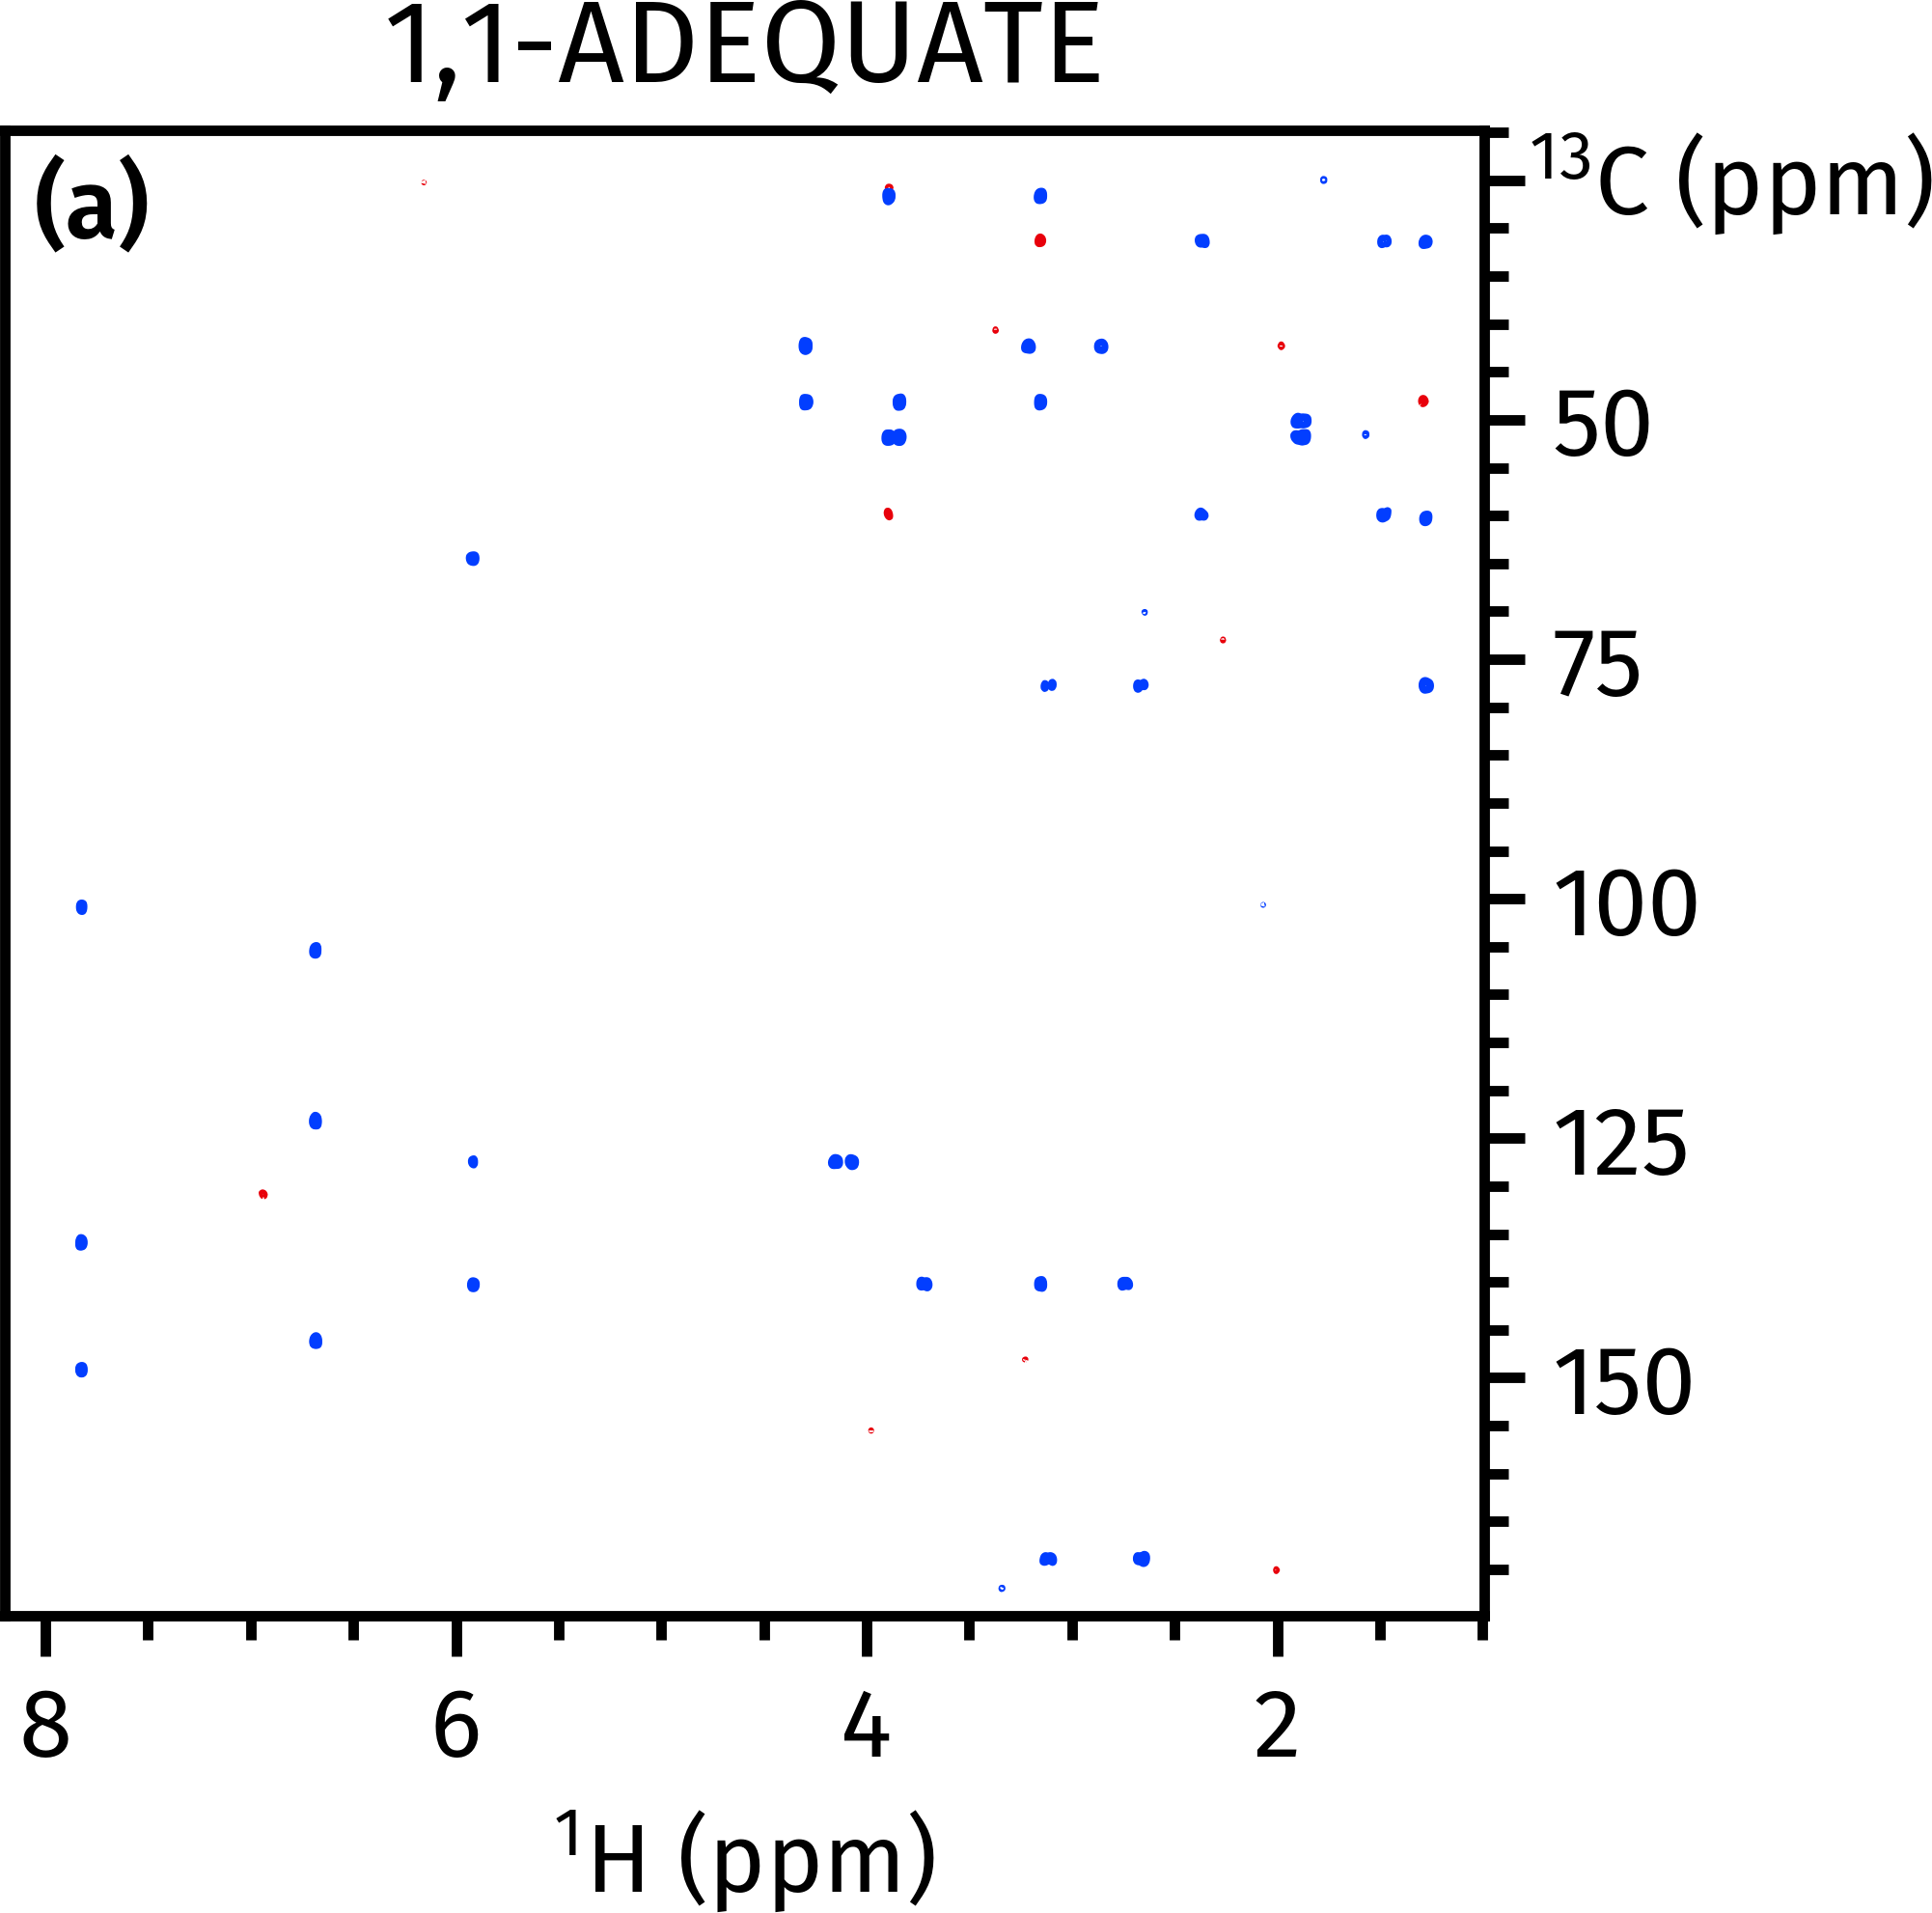
\includegraphics[]{abns_1.png}%
    \end{subfigure}
\end{figure}

\vspace{1cm}

\begin{figure}[htb]
    \ContinuedFloat
    \begin{subfigure}[b]{\textwidth}
        \centering
        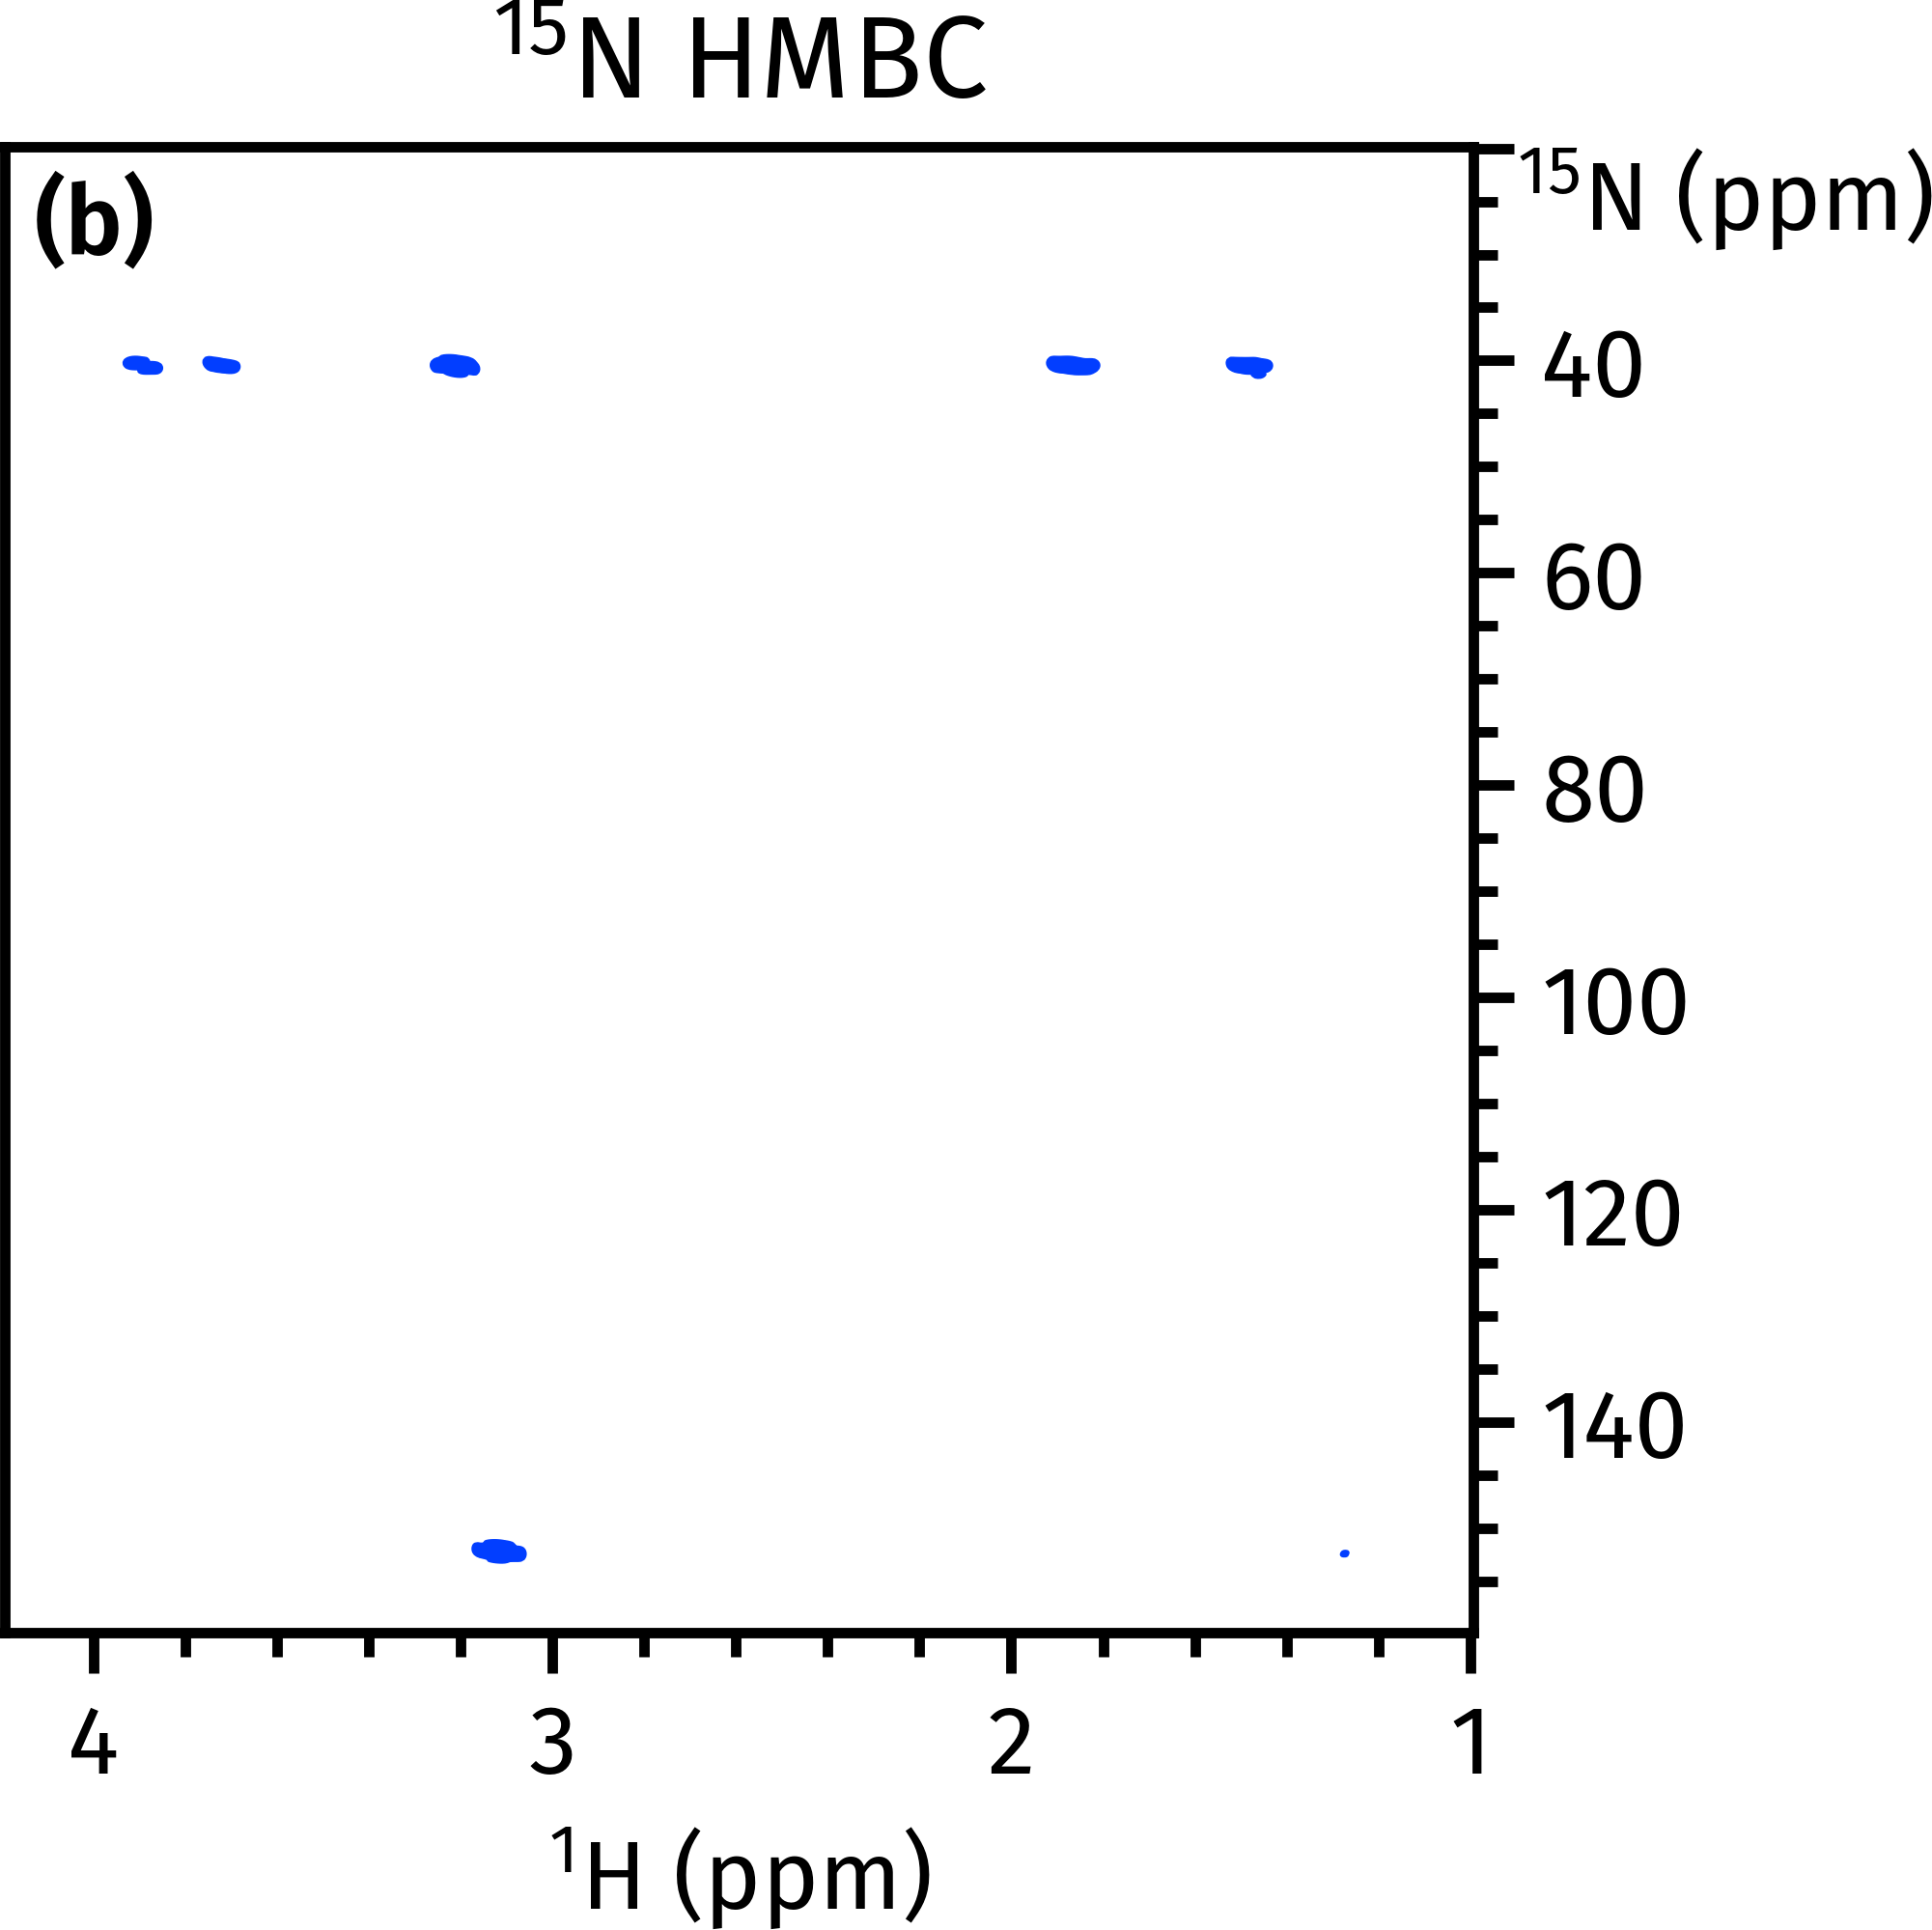
\includegraphics[]{abns_2.png}%
    \end{subfigure}
\end{figure}

\begin{figure}[htb]
    \ContinuedFloat
    \begin{subfigure}[b]{\textwidth}
        \centering
        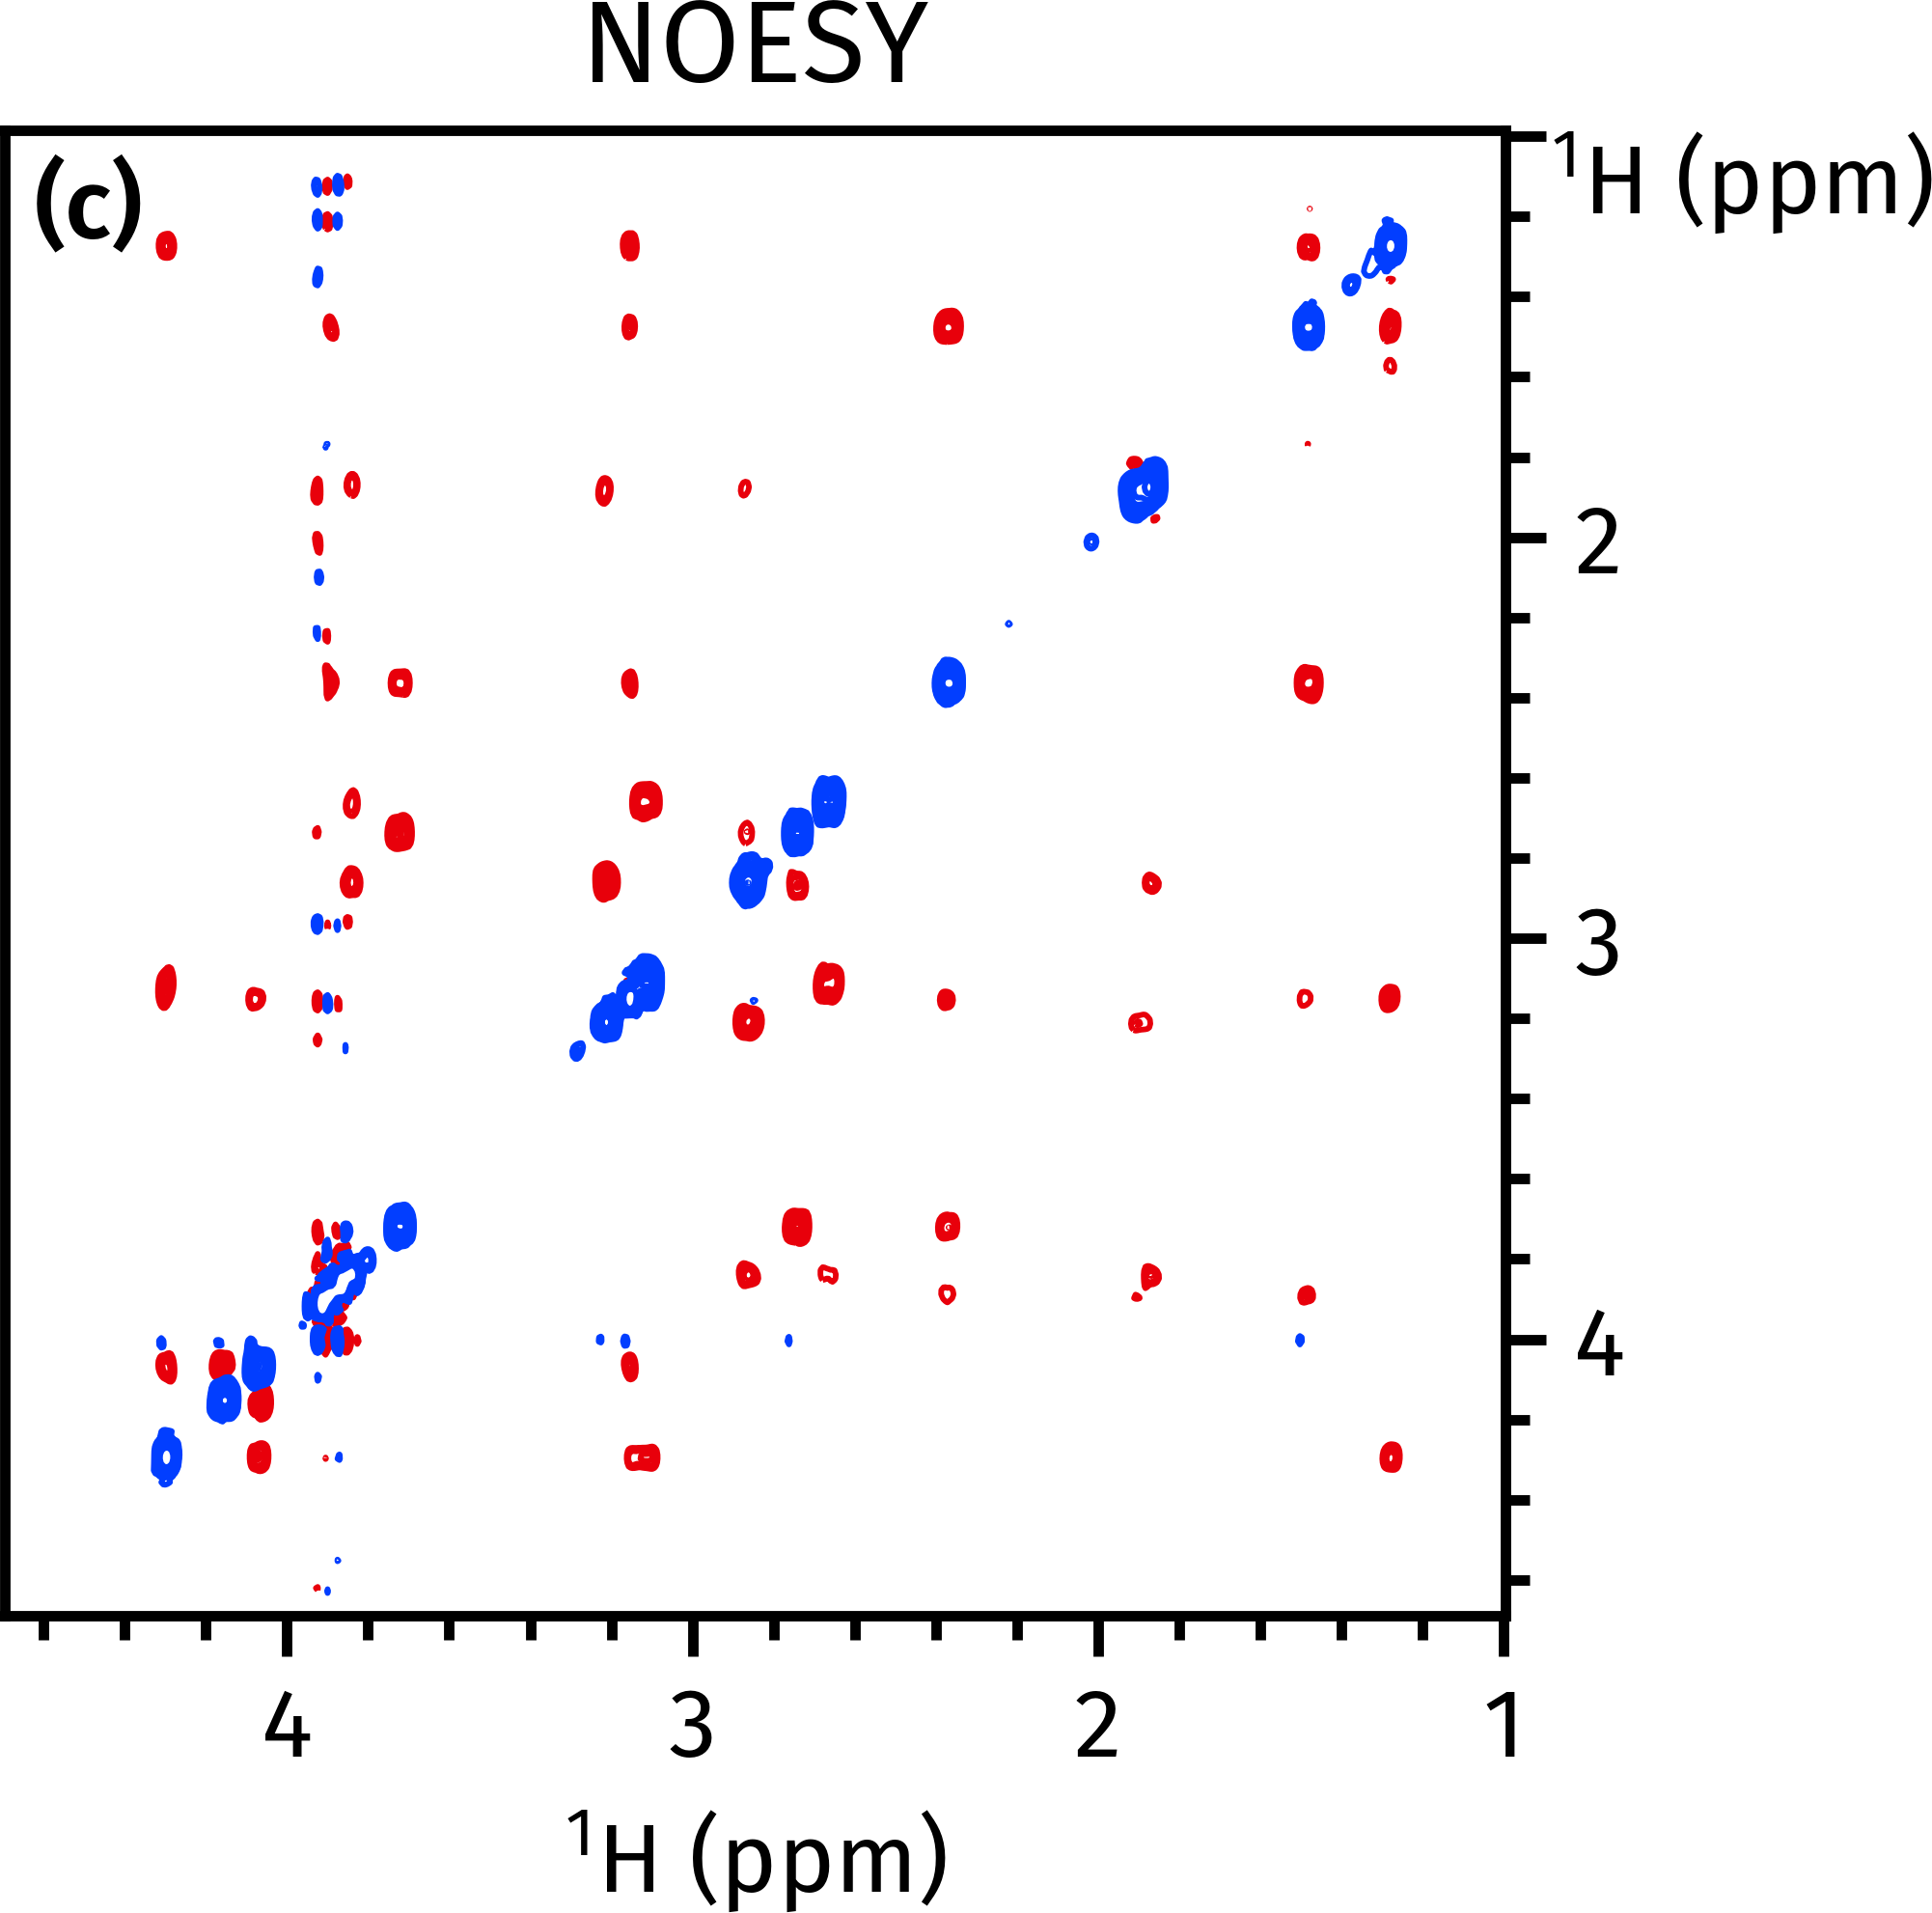
\includegraphics[]{abns_3.png}%
    \end{subfigure}
\end{figure}

\begin{figure}[htb]
    \ContinuedFloat
    \begin{subfigure}[b]{\textwidth}
        \centering
        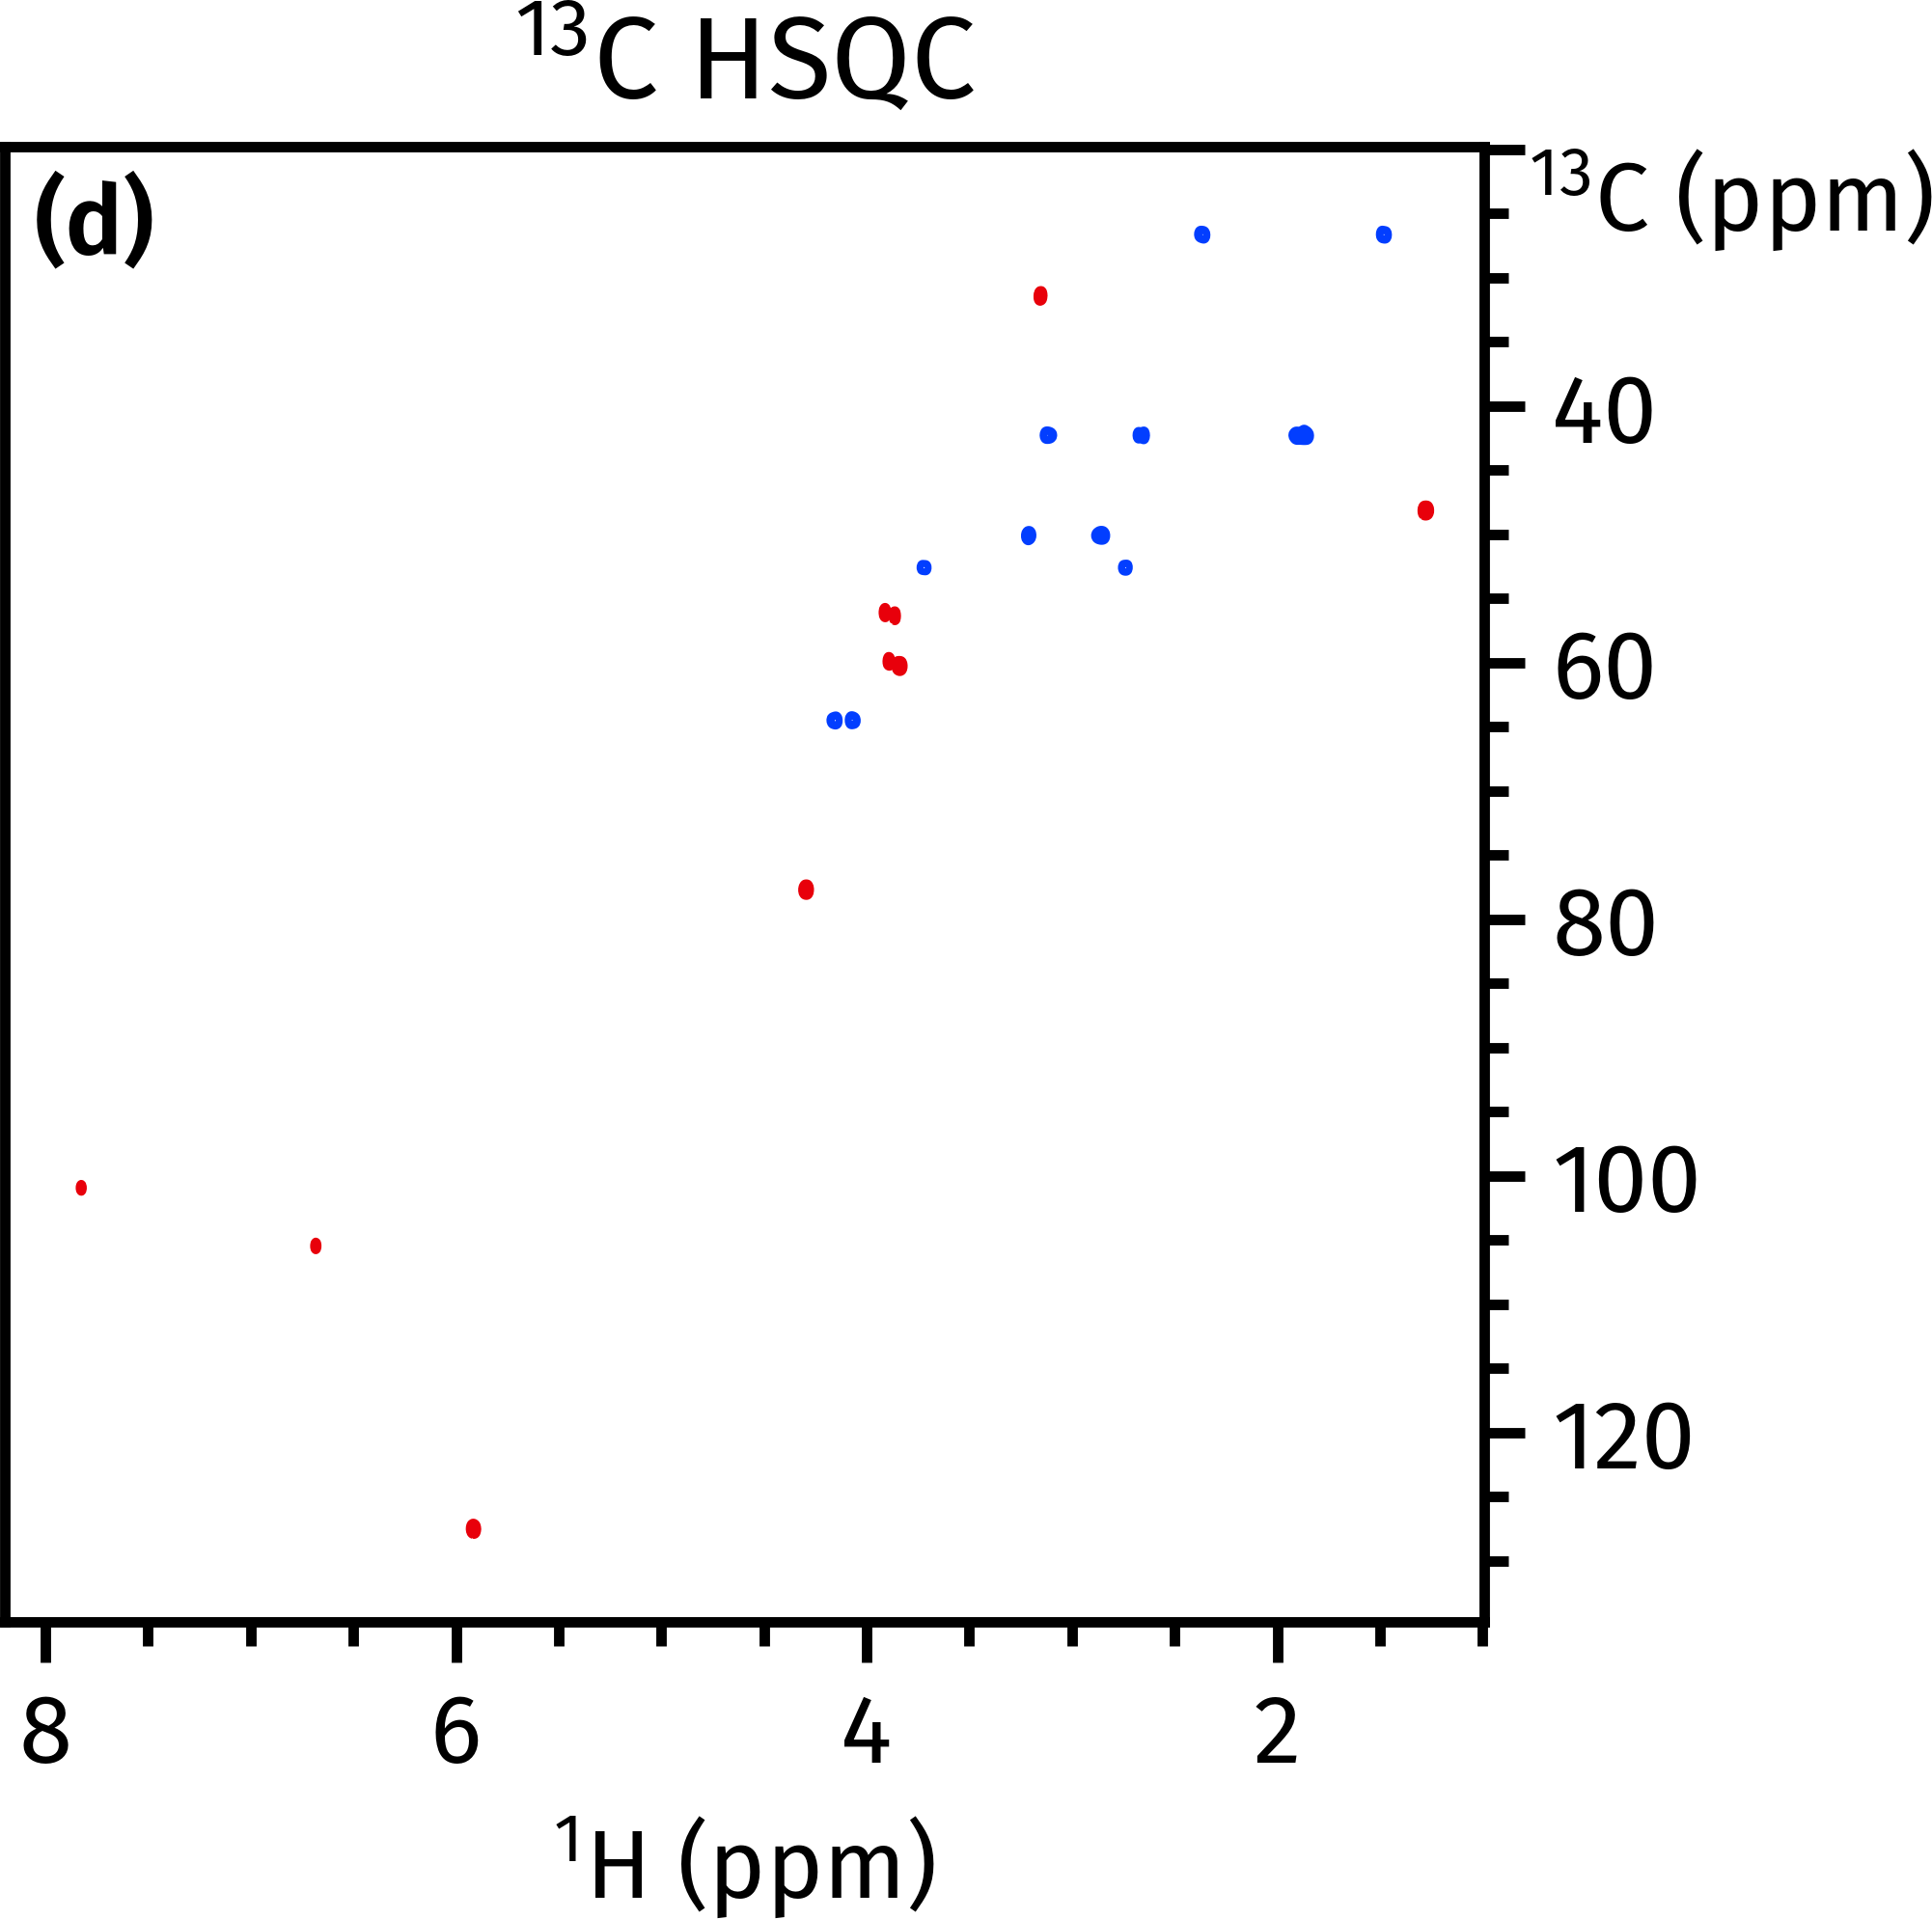
\includegraphics[]{abns_4.png}%
    \end{subfigure}
    {\phantomsubcaption\label{fig:abns_adeq}}
    {\phantomsubcaption\label{fig:abns_n_hmbc}}
    {\phantomsubcaption\label{fig:abns_c_hmbc}}
    {\phantomsubcaption\label{fig:abns_c_hsqc}}
    \caption{
        Spectra obtained from the \abnns{} supersequence.
        \textbf{(\subref*{fig:abns_adeq})} 1,1-ADEQUATE (16 transients).
        \textbf{(\subref*{fig:abns_n_hmbc})} \nitrogen{} HMBC (12 transients).
        \textbf{(\subref*{fig:abns_c_hmbc})} NOESY (2 transients, \SI{800}{\ms} mixing time).
        \textbf{(\subref*{fig:abns_c_hsqc})} \carbon{} HSQC (2 transients).
        \brucine{}.
    }
    \label{fig:abns}
\end{figure}

\clearpage
\section{\texorpdfstring{\abnbs{}}{NOAH-4 A(Bn/B/S)} comparison with and without DIPSI}
\label{sec:si_dipsi}

One additional feature of the \abnns{}, not described in the main text, concerns the fact that the \carbon{} HSQC module is placed immediately after the ADEQUATE (the second-last row in \cref{fig:abbs_pp}).
Both of these modules draw on the same \magn{\ch{C}} magnetisation pool, and this generally causes the latter module (here HSQC) to suffer from sensitivity losses.
Since the HSQC has a much greater intrinsic sensitivity compared to the ADEQUATE, this loss would in fact be tolerable.

In this experiment, we chose to also add a \qty{35}{\ms} period of isotropic DIPSI-2 mixing\autocite{Shaka1988JMR} immediately before the HSQC module (at the point marked with the red arrow in \cref{fig:abbs_pp}).
This effects \magnnot{\ch{C}} $\to$ \magn{\ch{C}} magnetisation transfer, and has previously been demonstrated in ASAP\autociteset{asaphsqc} and NOAH\autocite{Yong2021JMR} experiments.
Through this, some of the lost \magn{\ch{C}} magnetisation is replenished, leading to greater intensity in the HSQC (\cref{fig:dipsi}).
This mixing period does not need to be inserted prior to either of the \nitrogen{} or \carbon{} HMBC modules, as they do not use \magn{\ch{C}} magnetisation.
\Cref{fig:dipsi} compares the results obtained with and without this DIPSI block.

\begin{figure}[ht]
    \centering
    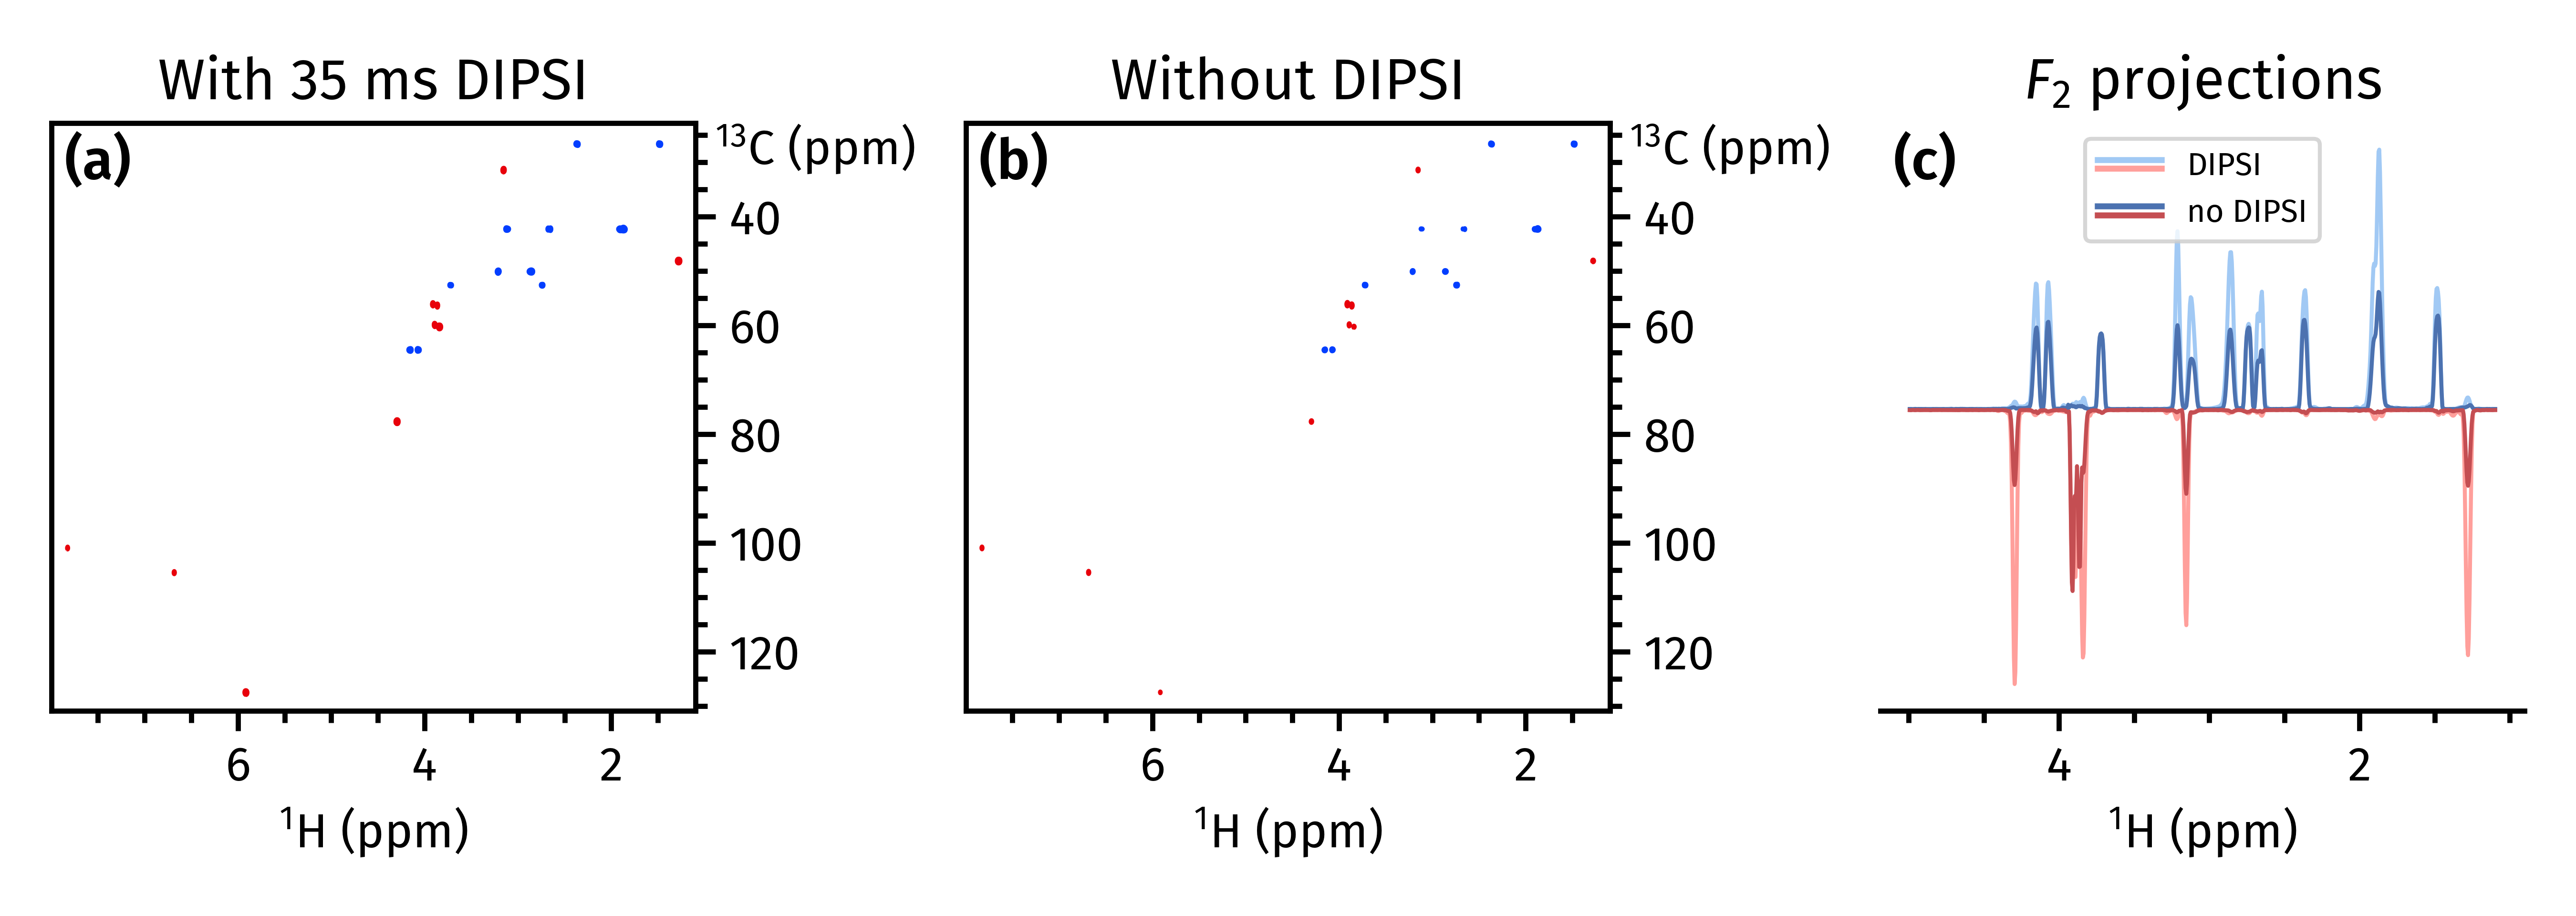
\includegraphics[]{dipsi.png}%
    {\phantomsubcaption\label{fig:dipsi_hsqc_dipsi}}
    {\phantomsubcaption\label{fig:dipsi_hsqc_nodipsi}}
    {\phantomsubcaption\label{fig:dipsi_projections}}
    \caption{
        \carbon{} HSQC spectra obtained from the \abnbs{} experiment (\cref{fig:sequences_abbs}).
        \textbf{(\subref*{fig:dipsi_hsqc_dipsi})} With \SI{35}{\ms} DIPSI mixing between the ADEQUATE and \carbon{} HSQC modules (this spectrum is the same as in \cref{fig:abbs_c_hsqc}).
        \textbf{(\subref*{fig:dipsi_hsqc_nodipsi})} Without DIPSI mixing between the ADEQUATE and \carbon{} HSQC modules.
        \textbf{(\subref*{fig:dipsi_projections})} Projections of the spectra in (\subref*{fig:dipsi_hsqc_dipsi}) and (\subref*{fig:dipsi_hsqc_nodipsi}) onto the $F_2$ axis.
        \brucine{}.
    }
    \label{fig:dipsi}
\end{figure}

The spectral quality in both cases is acceptable.
However, the spectrum acquired without DIPSI mixing (\cref{fig:dipsi_hsqc_dipsi}) is weaker, which is more clearly shown in the projections onto the $F_2$ axes (\cref{fig:dipsi_projections}).
When DIPSI mixing is added, the average signal enhancement across all peaks in the HSQC is 88\% (\cref{fig:dipsi}).
These observations are consistent with previous studies on NOAH supersequences containing two successive \magn{\ch{C}} modules.\autocite{Yong2021JMR}

\clearpage

\section{Spectra from \texorpdfstring{\abnbspns{}}{NOAH-5 A(Bn/B/Spn/S)}}

\begin{figure}[ht]
    \centering
    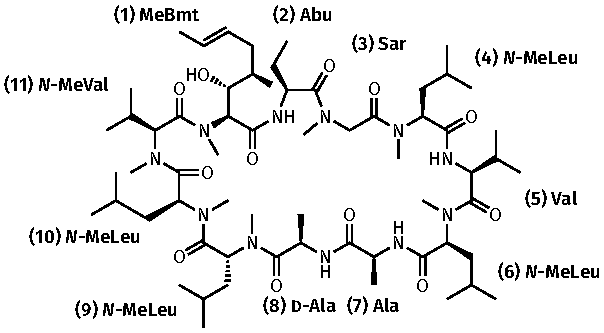
\includegraphics[draft=false]{figures/cyclosporin.pdf}%
    \caption[Structure of cyclosporin]{
        Structure of cyclosporin with residues numbered.
    }
    \label{fig:samples_cyclosporin}
\end{figure}

\begin{figure}[htb]
    \begin{subfigure}[b]{\textwidth}
        \centering
        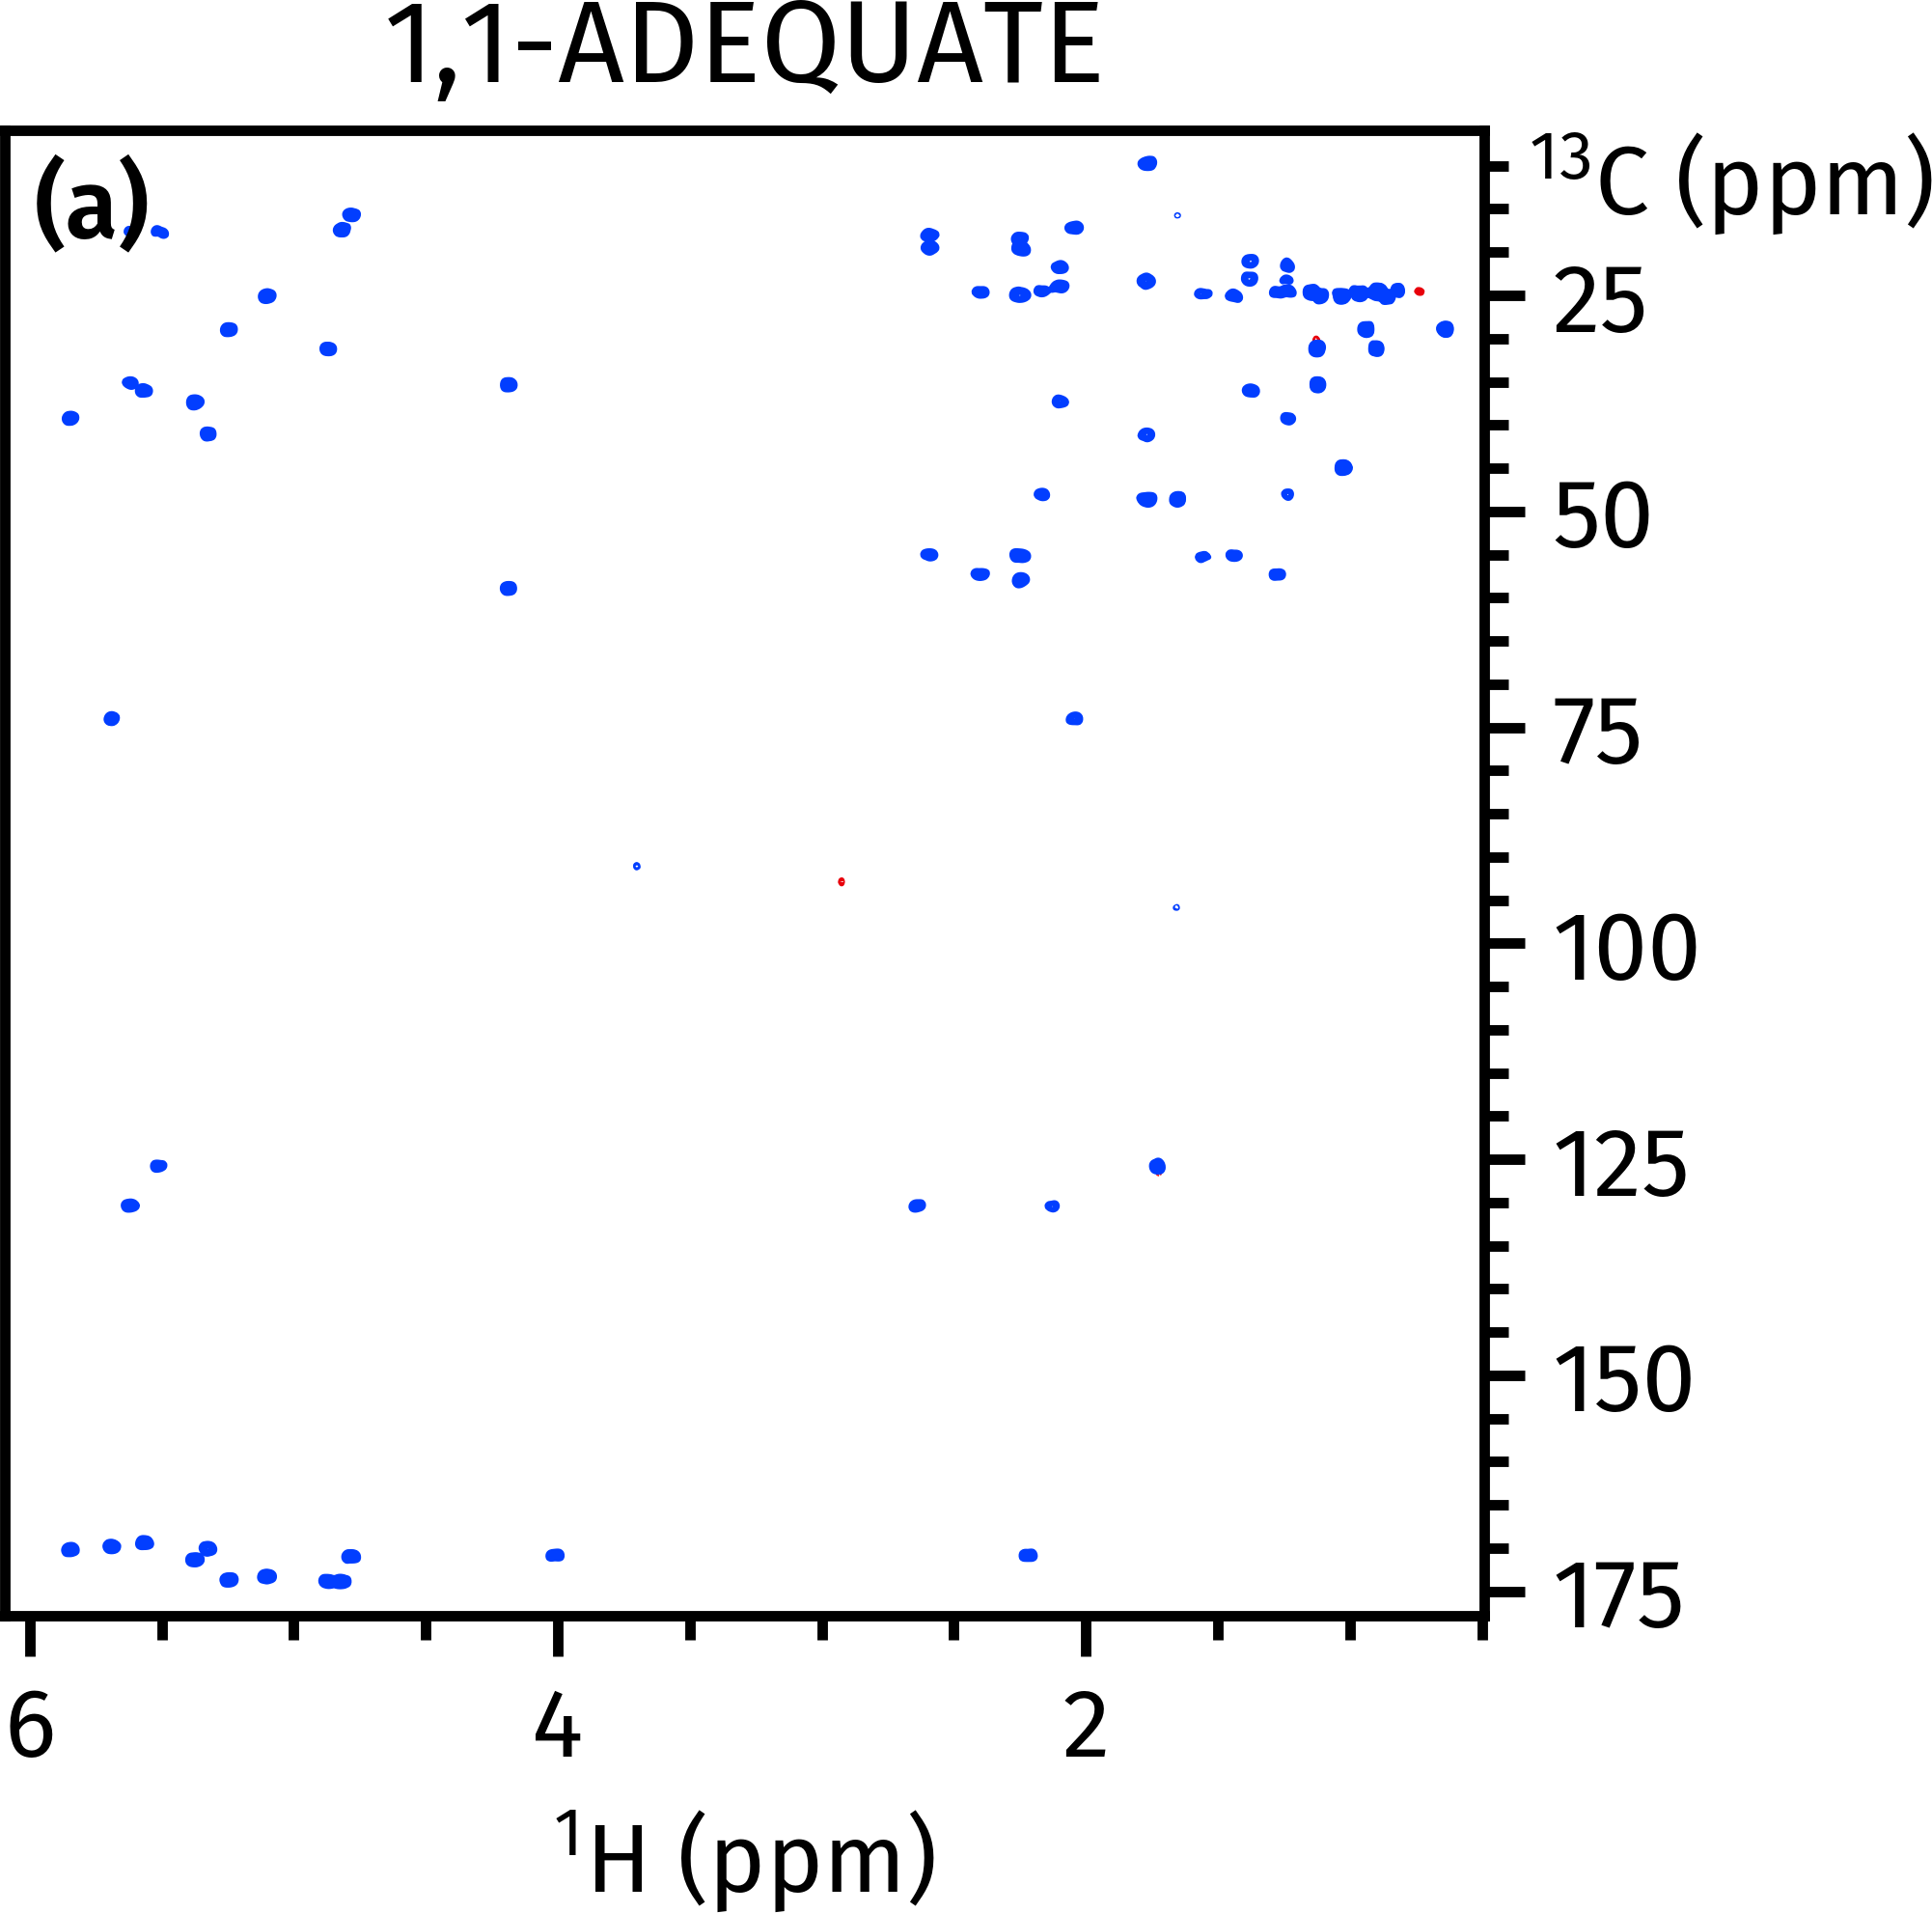
\includegraphics[]{abbss_1.png}%
    \end{subfigure}
\end{figure}
\begin{figure}[htb]
    \ContinuedFloat
    \begin{subfigure}[b]{\textwidth}
        \centering
        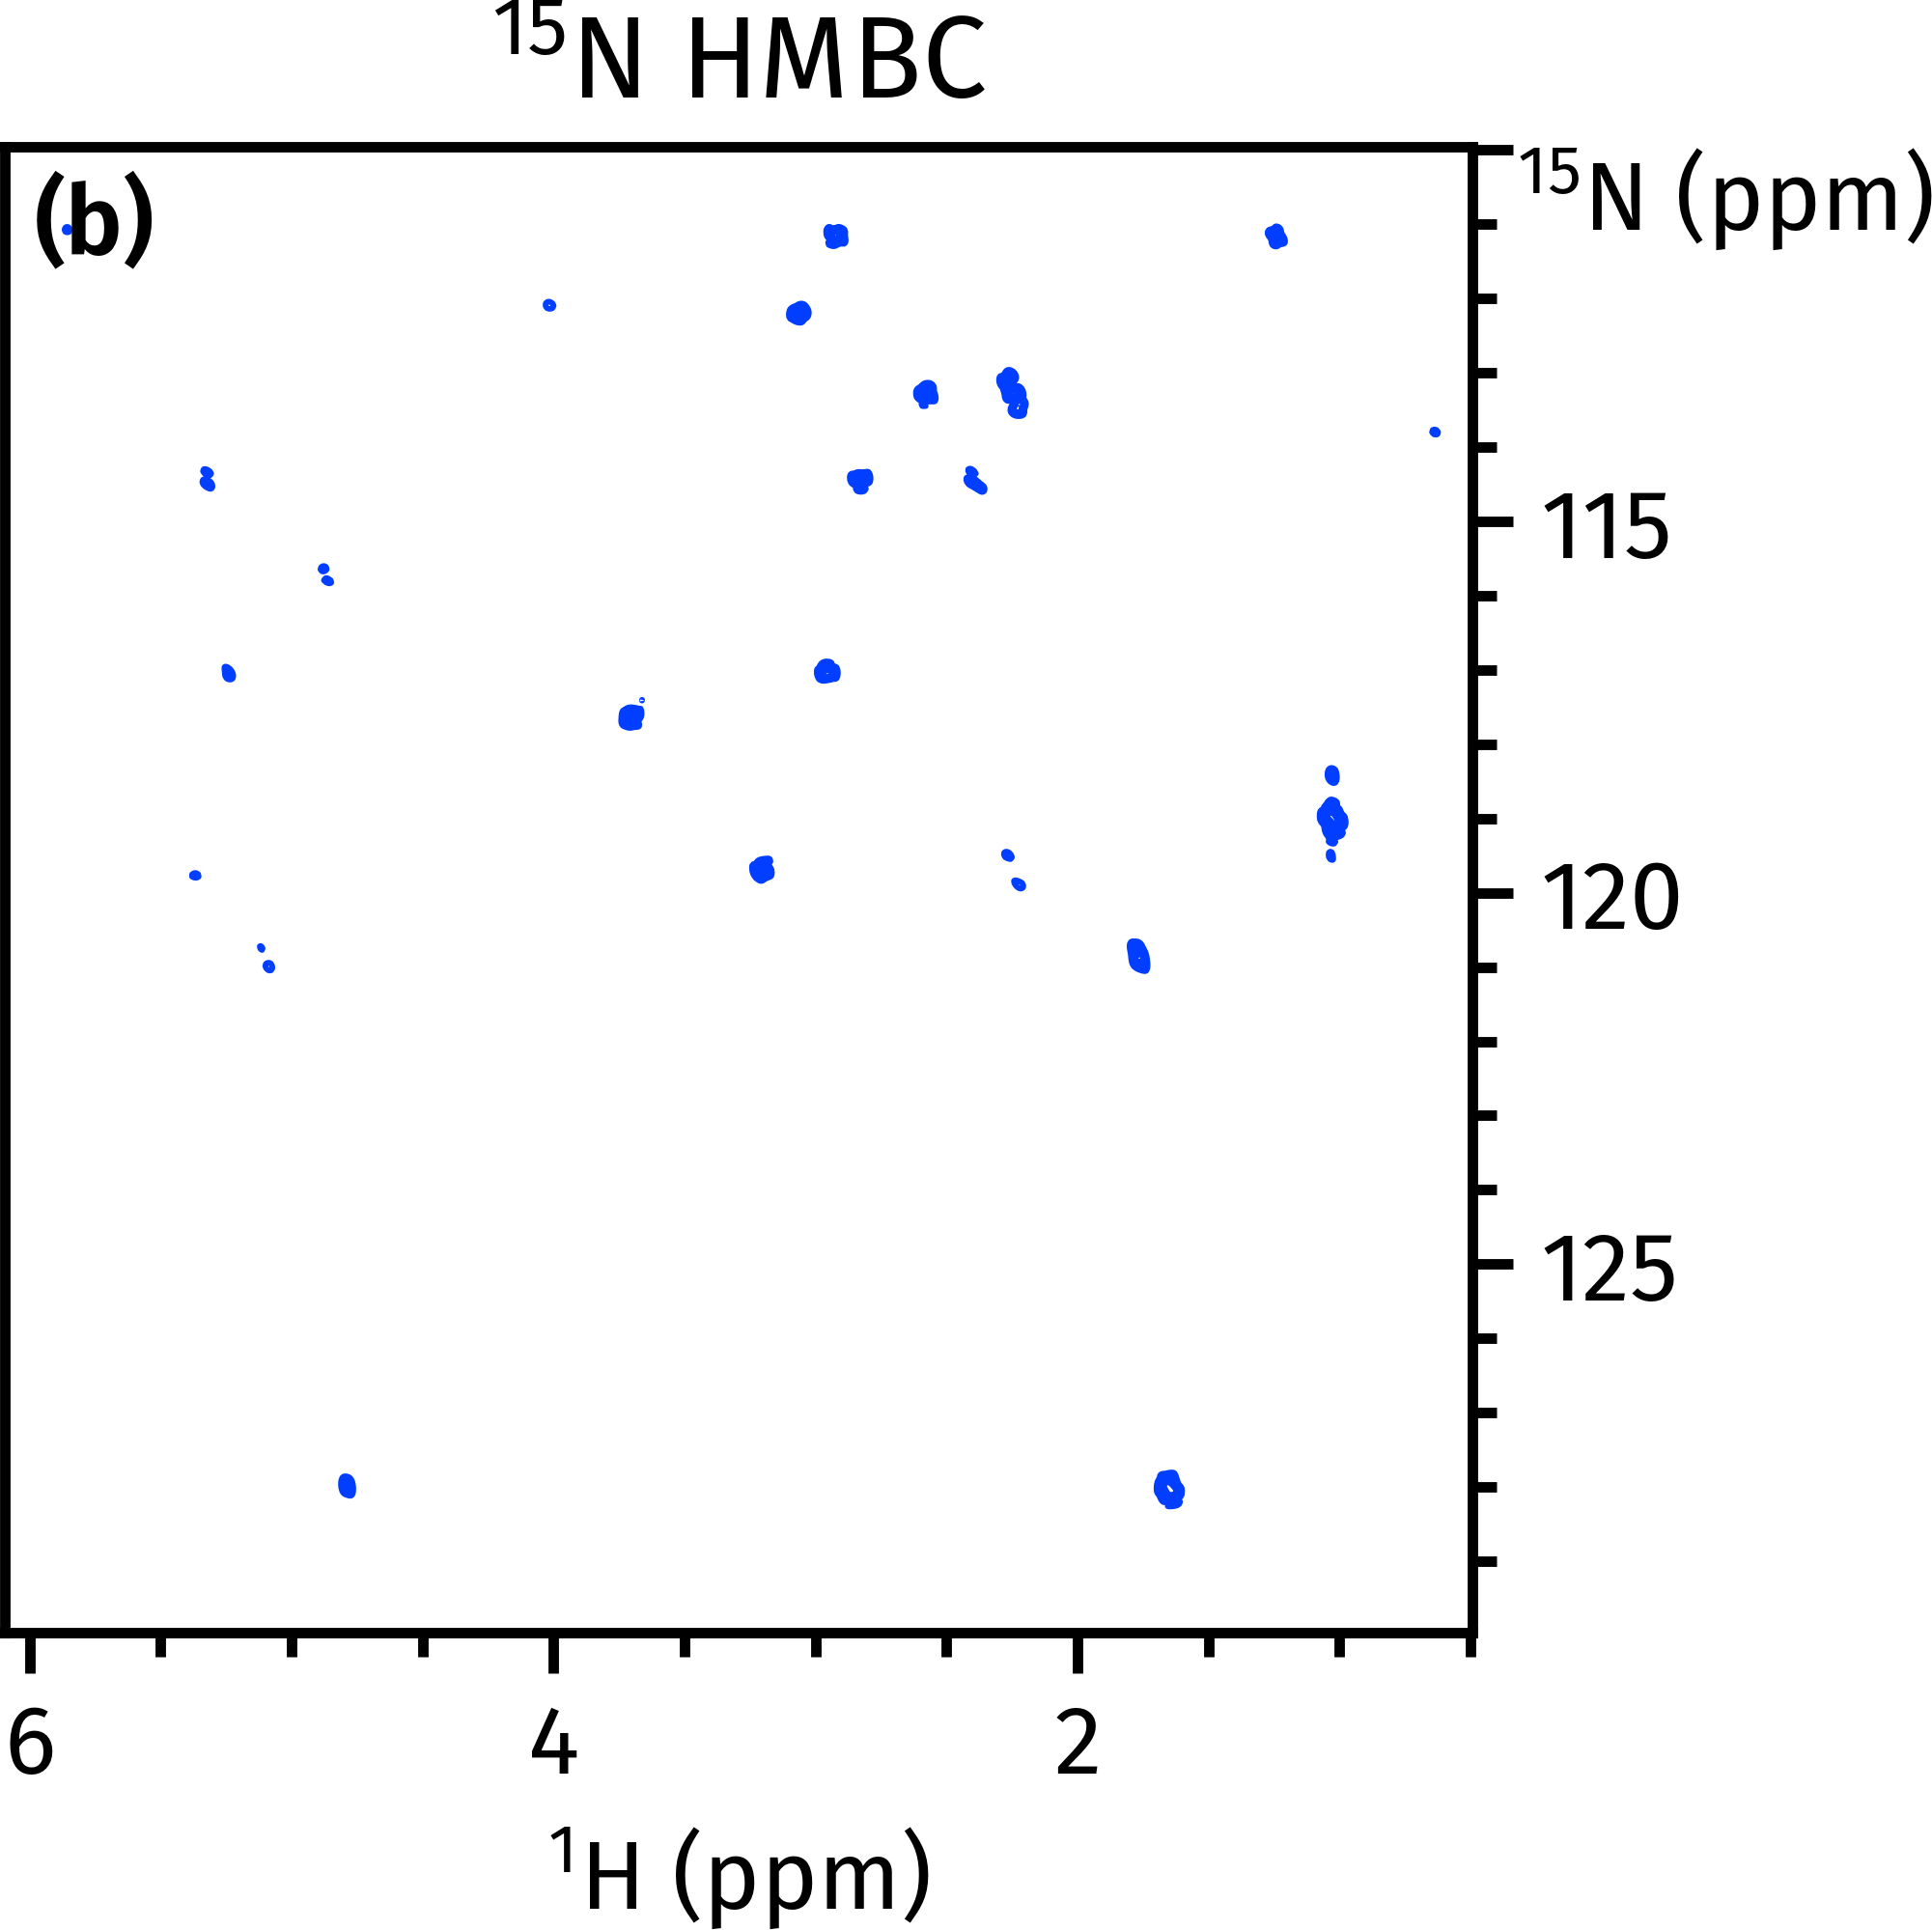
\includegraphics[]{abbss_2.png}%
    \end{subfigure}
\end{figure}
\begin{figure}[htb]
    \ContinuedFloat
    \begin{subfigure}[b]{\textwidth}
        \centering
        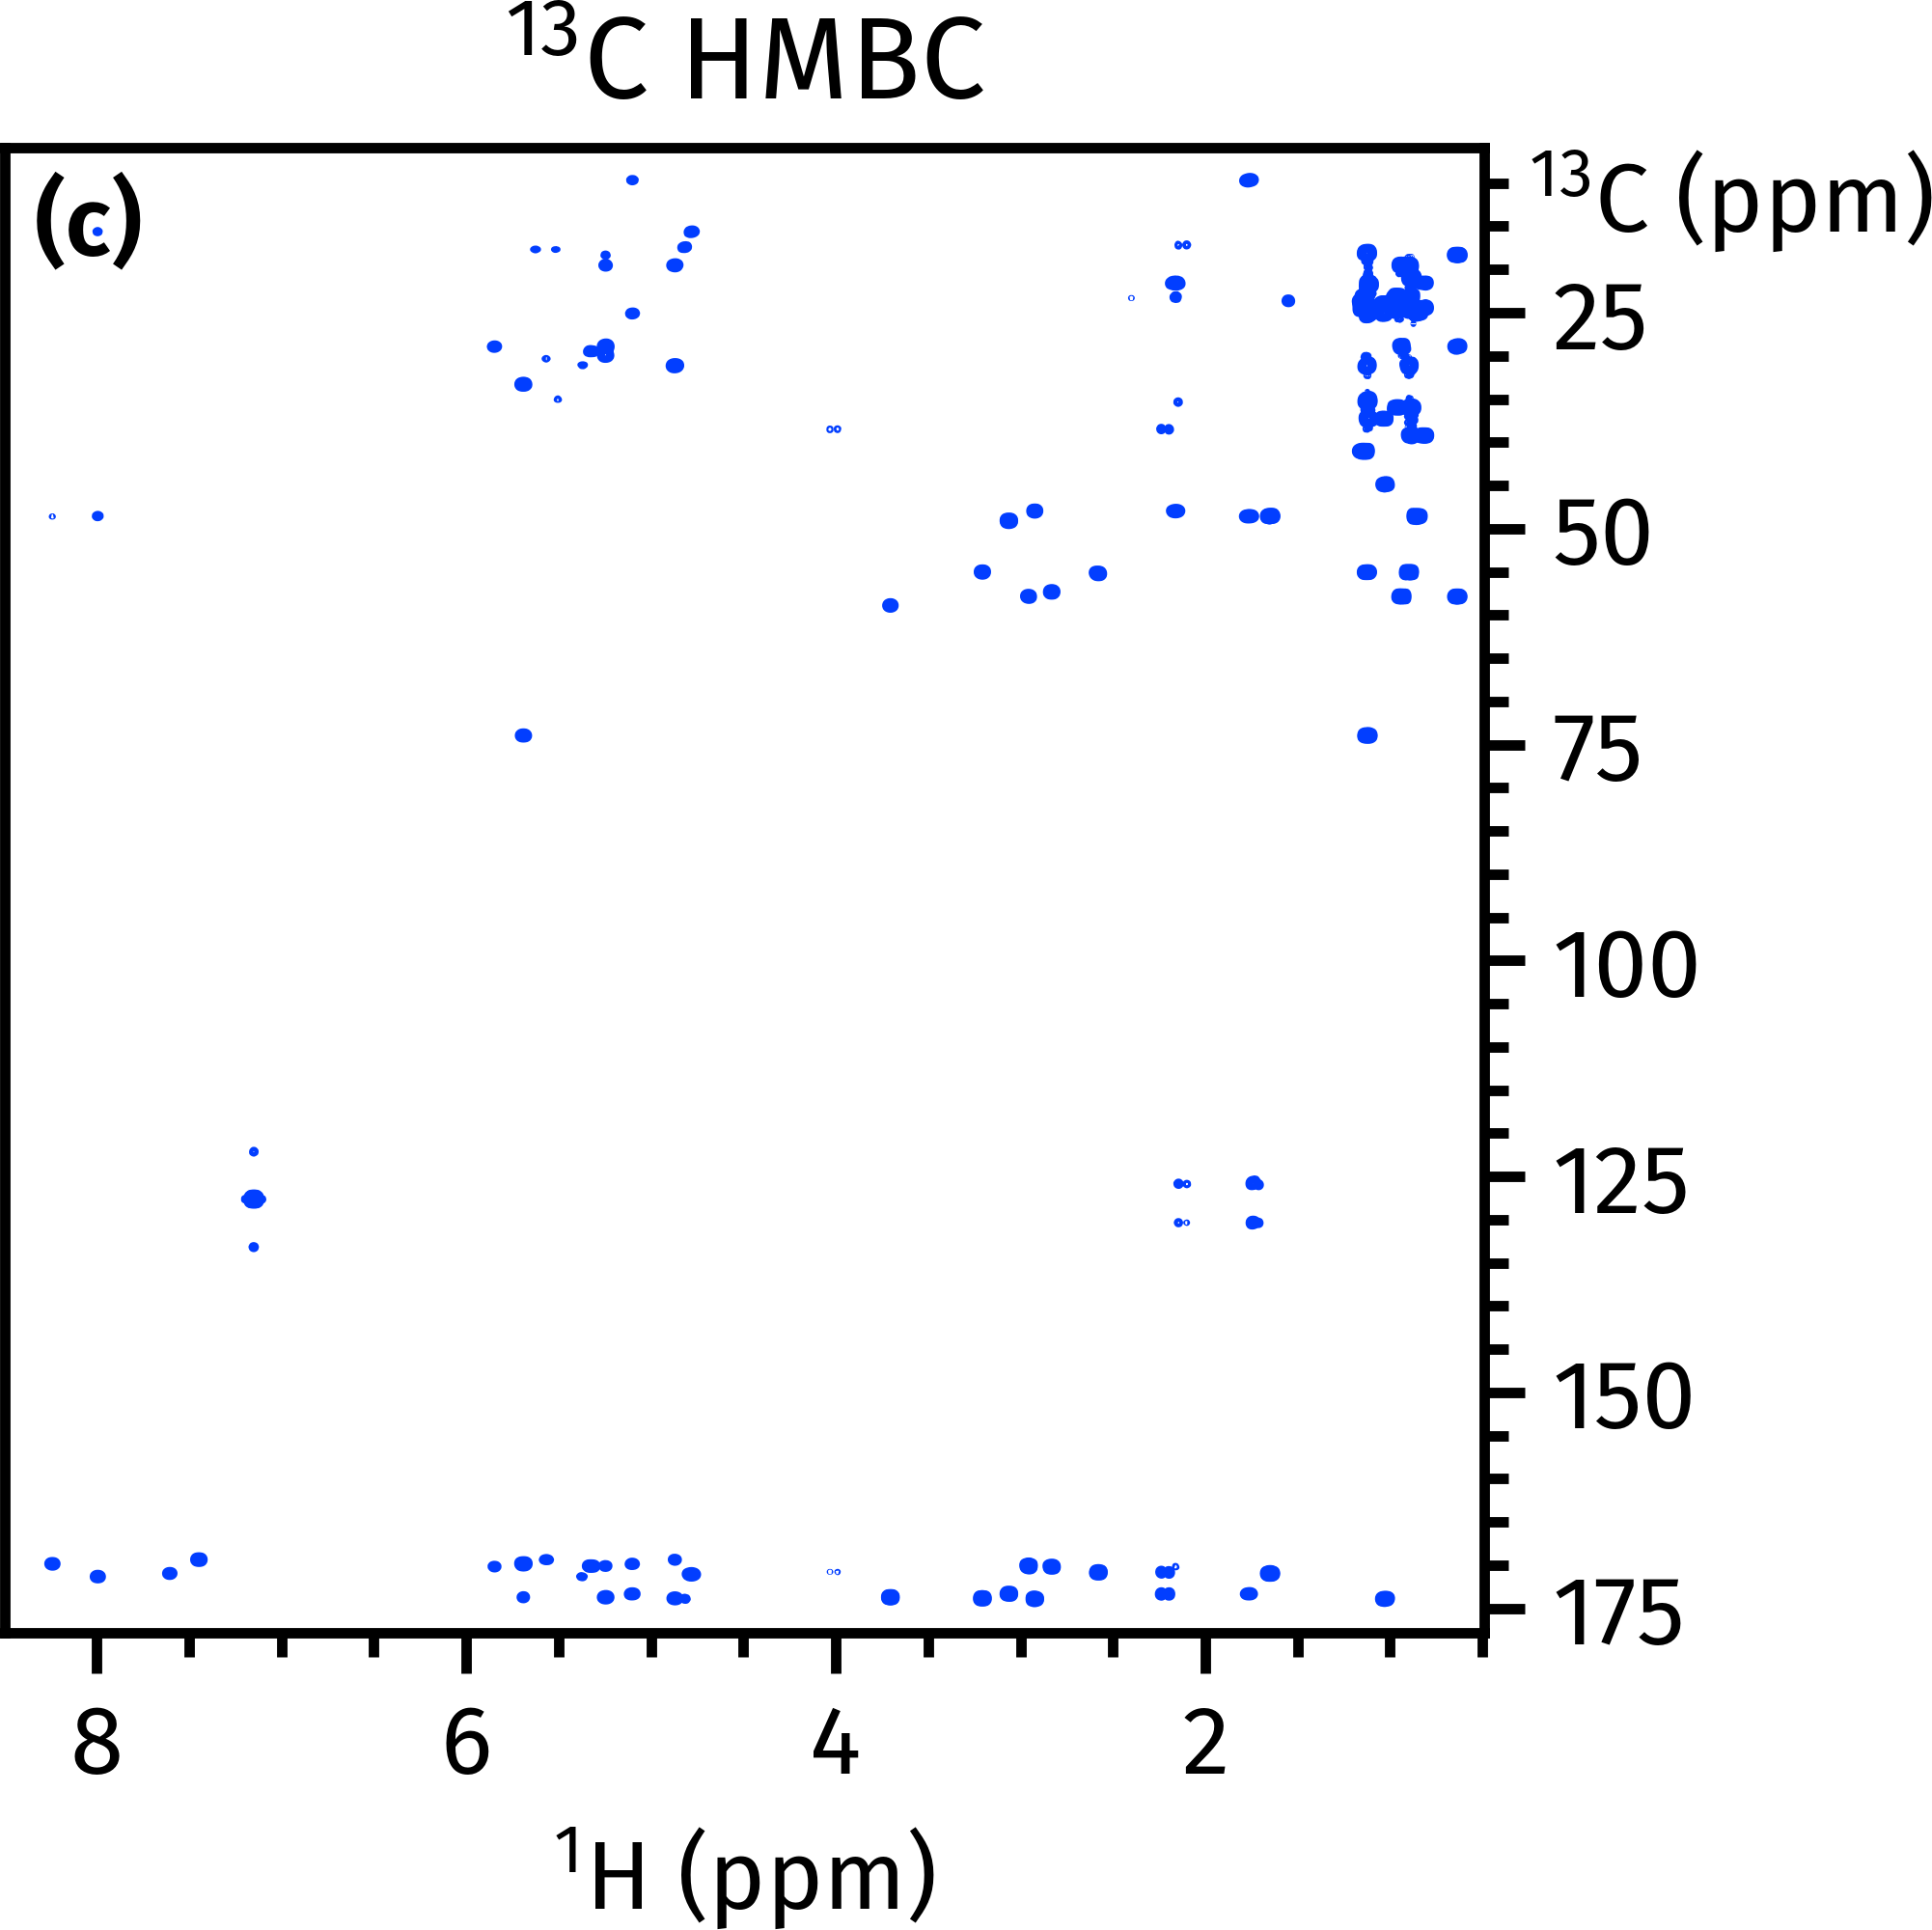
\includegraphics[]{abbss_3.png}%
    \end{subfigure}
\end{figure}
\begin{figure}[htb]
    \ContinuedFloat
    \begin{subfigure}[b]{\textwidth}
        \centering
        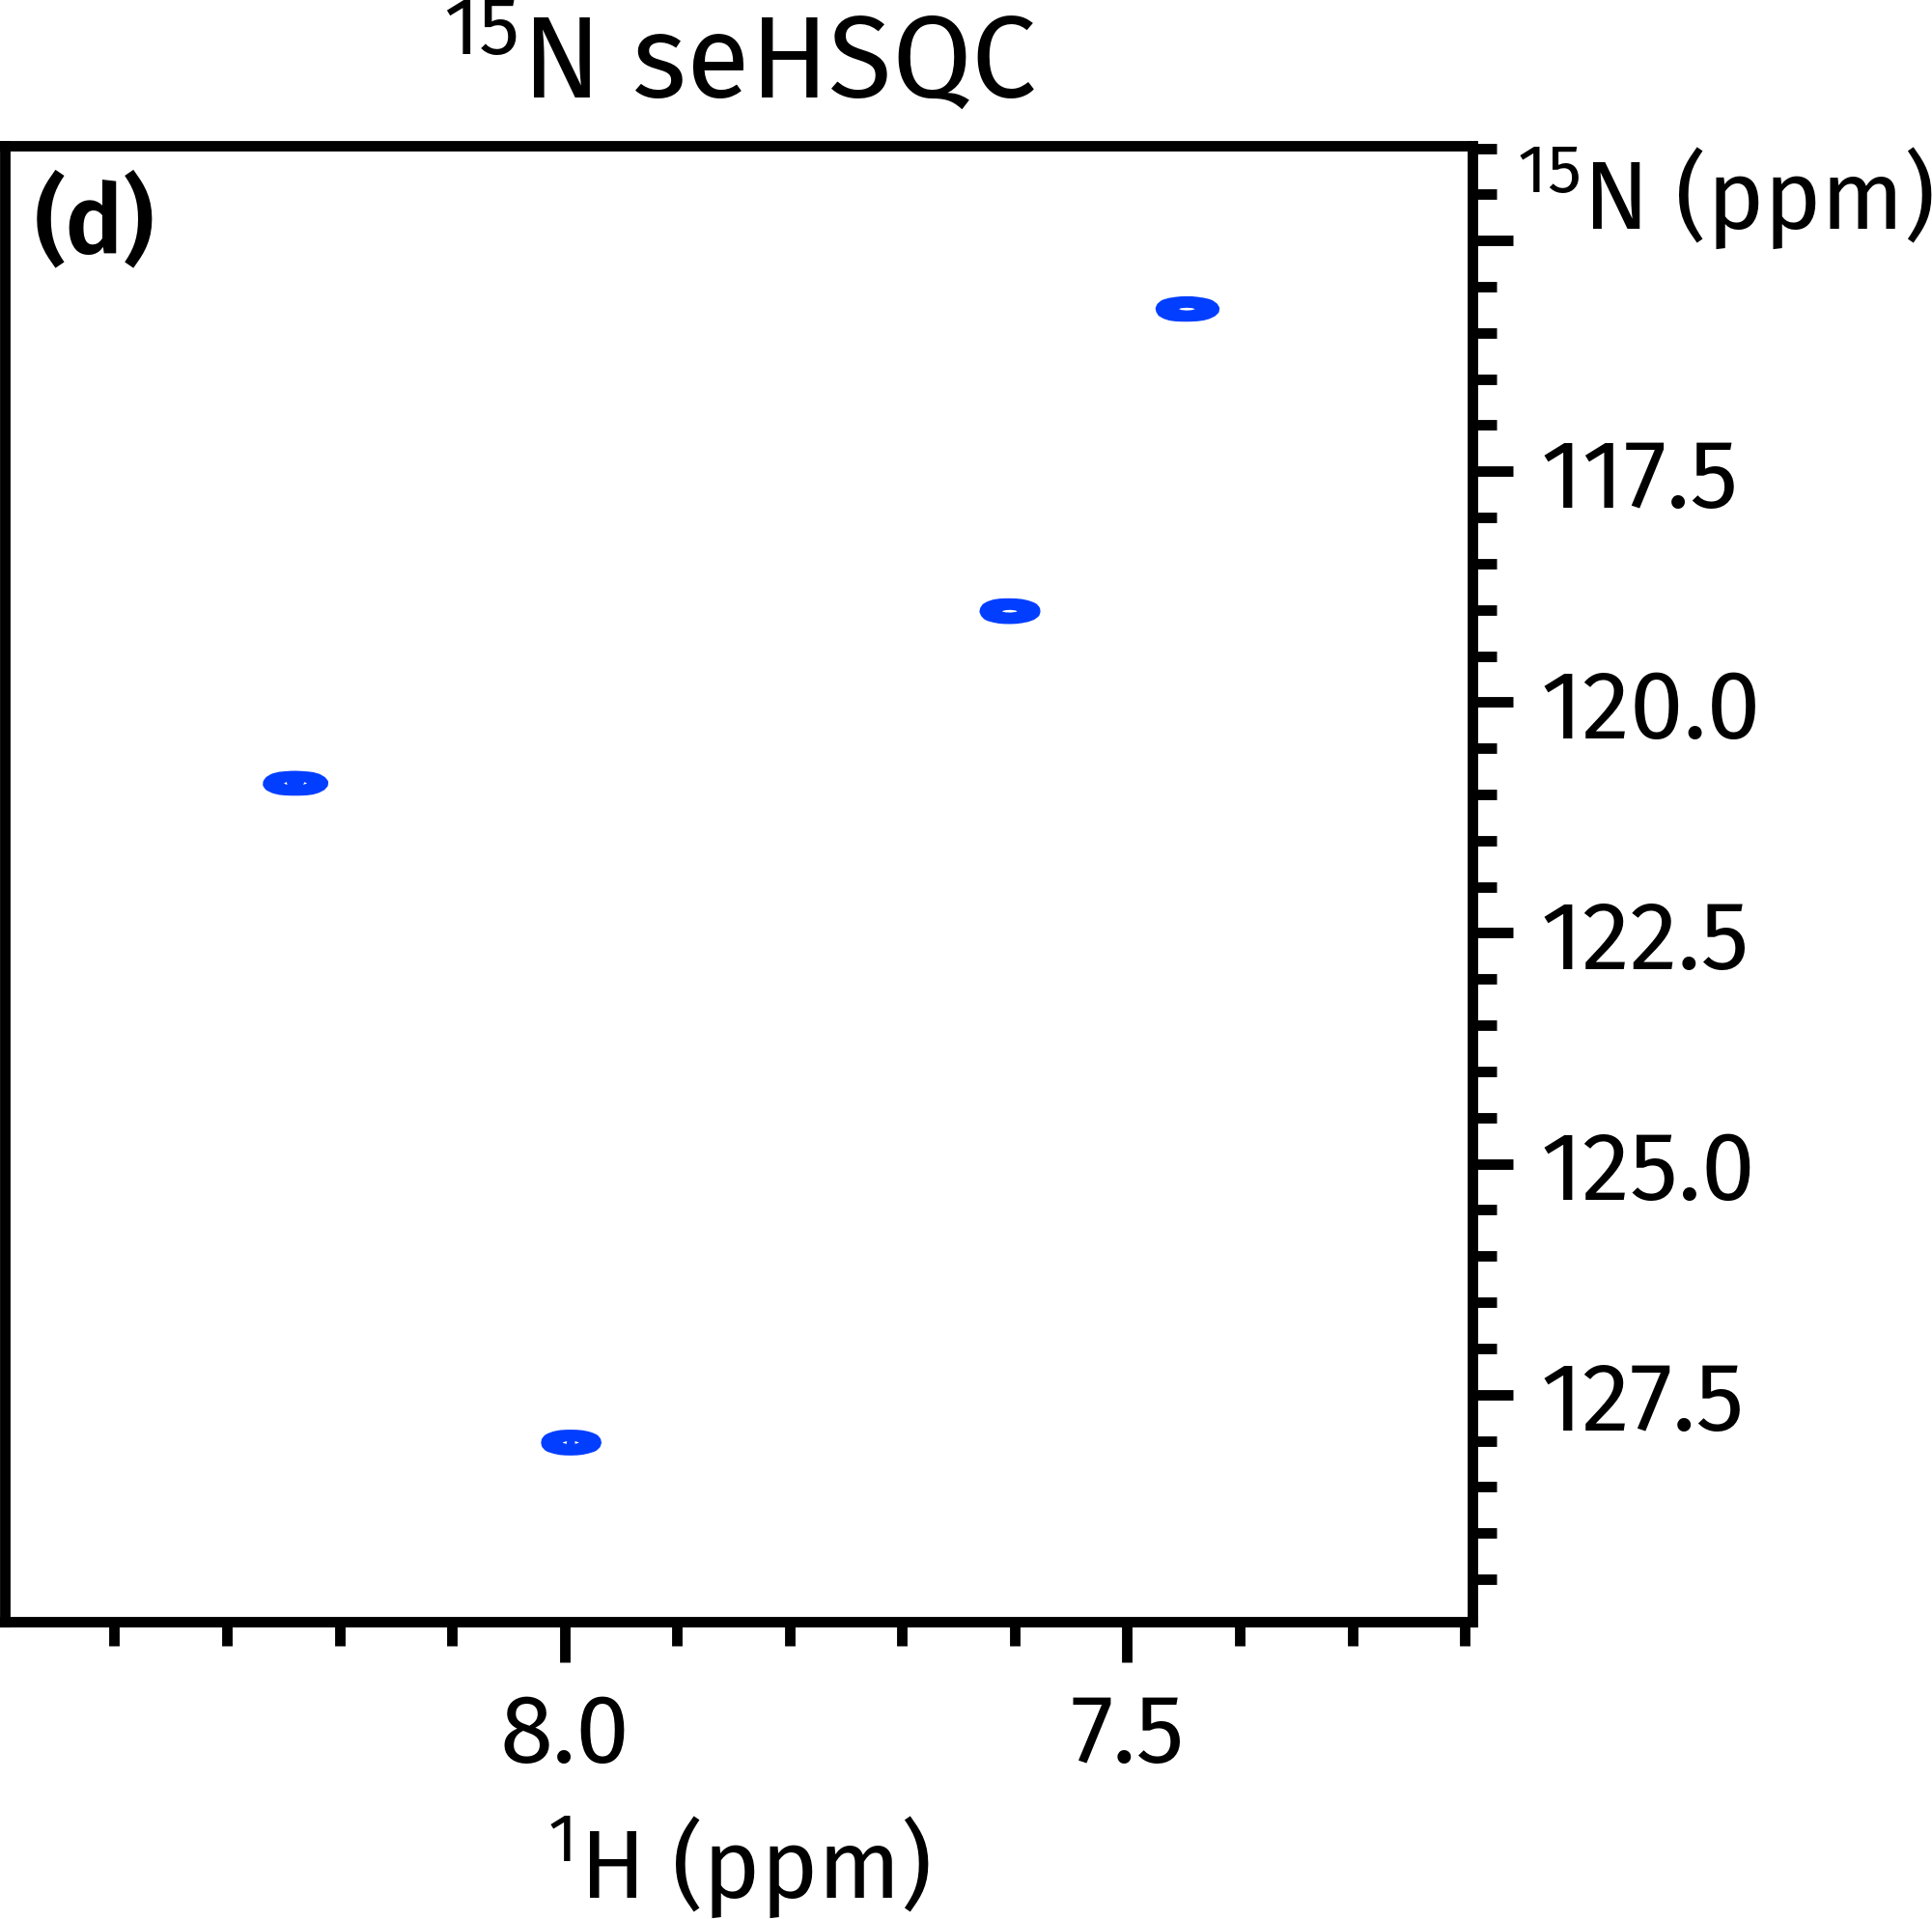
\includegraphics[]{abbss_4.png}%
    \end{subfigure}
\end{figure}

\begin{figure}[htb]
    \ContinuedFloat
    \begin{subfigure}[b]{\textwidth}
        \centering
        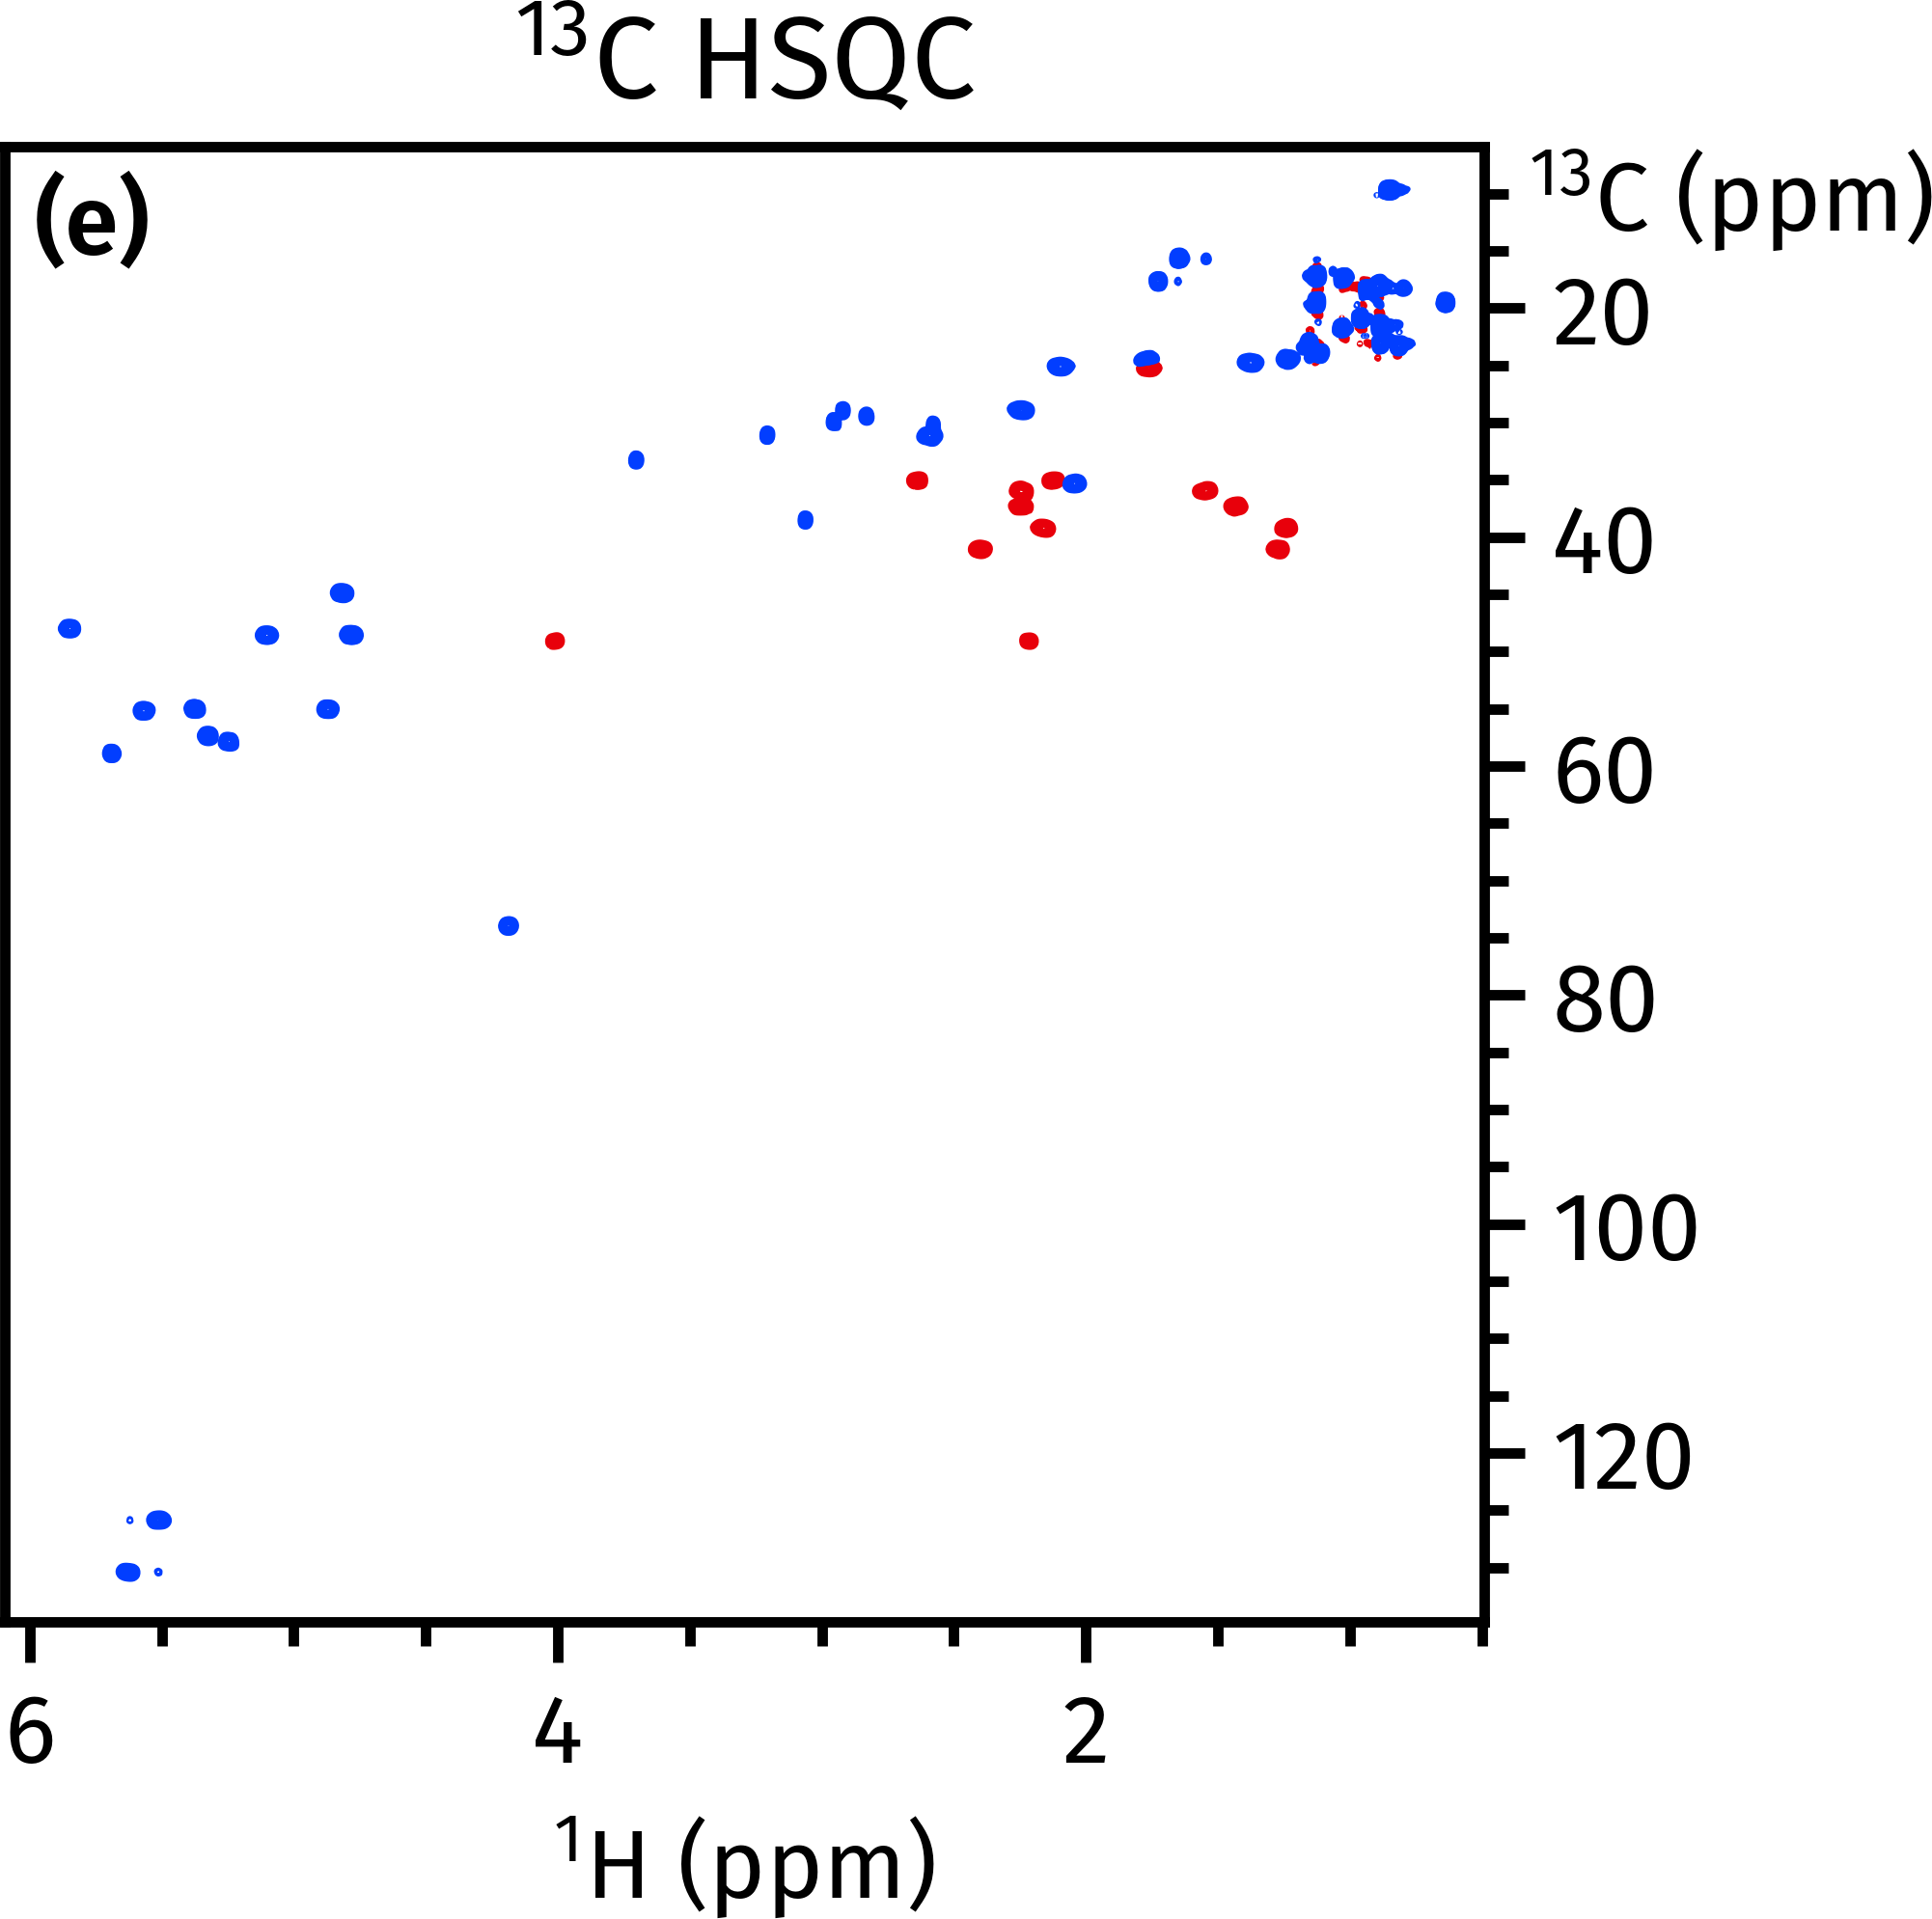
\includegraphics[]{abbss_5.png}%
    \end{subfigure}
    {\phantomsubcaption\label{fig:abbss_adeq}}
    {\phantomsubcaption\label{fig:abbss_n_hmbc}}
    {\phantomsubcaption\label{fig:abbss_c_hmbc}}
    {\phantomsubcaption\label{fig:abbss_n_sehsqc}}
    {\phantomsubcaption\label{fig:abbss_c_hsqc}}
    \caption{
        Spectra obtained from the \abnbspns{} supersequence.
        All modules were recorded with 256 $t_1$ increments.
        \textbf{(\subref*{fig:abbss_adeq})} 1,1-ADEQUATE (16 transients).
        \textbf{(\subref*{fig:abbss_n_hmbc})} \nitrogen{} HMBC (10 transients).
        \textbf{(\subref*{fig:abbss_c_hmbc})} \carbon{} HMBC (2 transients).
        \textbf{(\subref*{fig:abbss_n_sehsqc})} \nitrogen{} sensitivity-enhanced HSQC (2 transients).
        \textbf{(\subref*{fig:abbss_c_hsqc})} \carbon{} HSQC (2 transients).
        \cyclo{}.
    }
    \label{fig:abbss}
\end{figure}

\clearpage

\section{Covariance spectra from \texorpdfstring{\abnbspns{}}{NOAH-5 A(Bn/B/Spn/S)}}
\label{sec:si_covariance}

The heteronuclear spectra obtained from the \abnbspns{} supersequence can be processed using indirect covariance processing\autociteset{indirect-covariance} to yield other forms of correlation spectra.
For example, the \nitrogen{} HMBC and \carbon{} HSQC can be used to generate \carbon{}--\nitrogen{} correlation spectra (\cref{fig:covariance_brucine_nc}).\autocite{Kupce2007MRC,Martin2007JHC,Martin2007MRC}
Furthermore, the \carbon{} HSQC and ADEQUATE experiments can be used to create \carbon{}--\carbon{} one-bond correlation spectra (\cref{fig:covariance_cyclo_caco,fig:covariance_cyclo_sidechain}).\autociteset{hsqc-adequate}
It should be further emphasised that all of the `base' spectra used as the inputs here are obtained \textit{in a single measurement} using either the NOAH-4 or NOAH-5 supersequences discussed above.
A notable benefit of this is that $t_1$ for all modules are incremented simultaneously: this minimises the effects of temporal variations such as temperature drifts, which can lead to inaccurate peaks in covariance spectra.

\begin{figure}[ht]
    \centering
    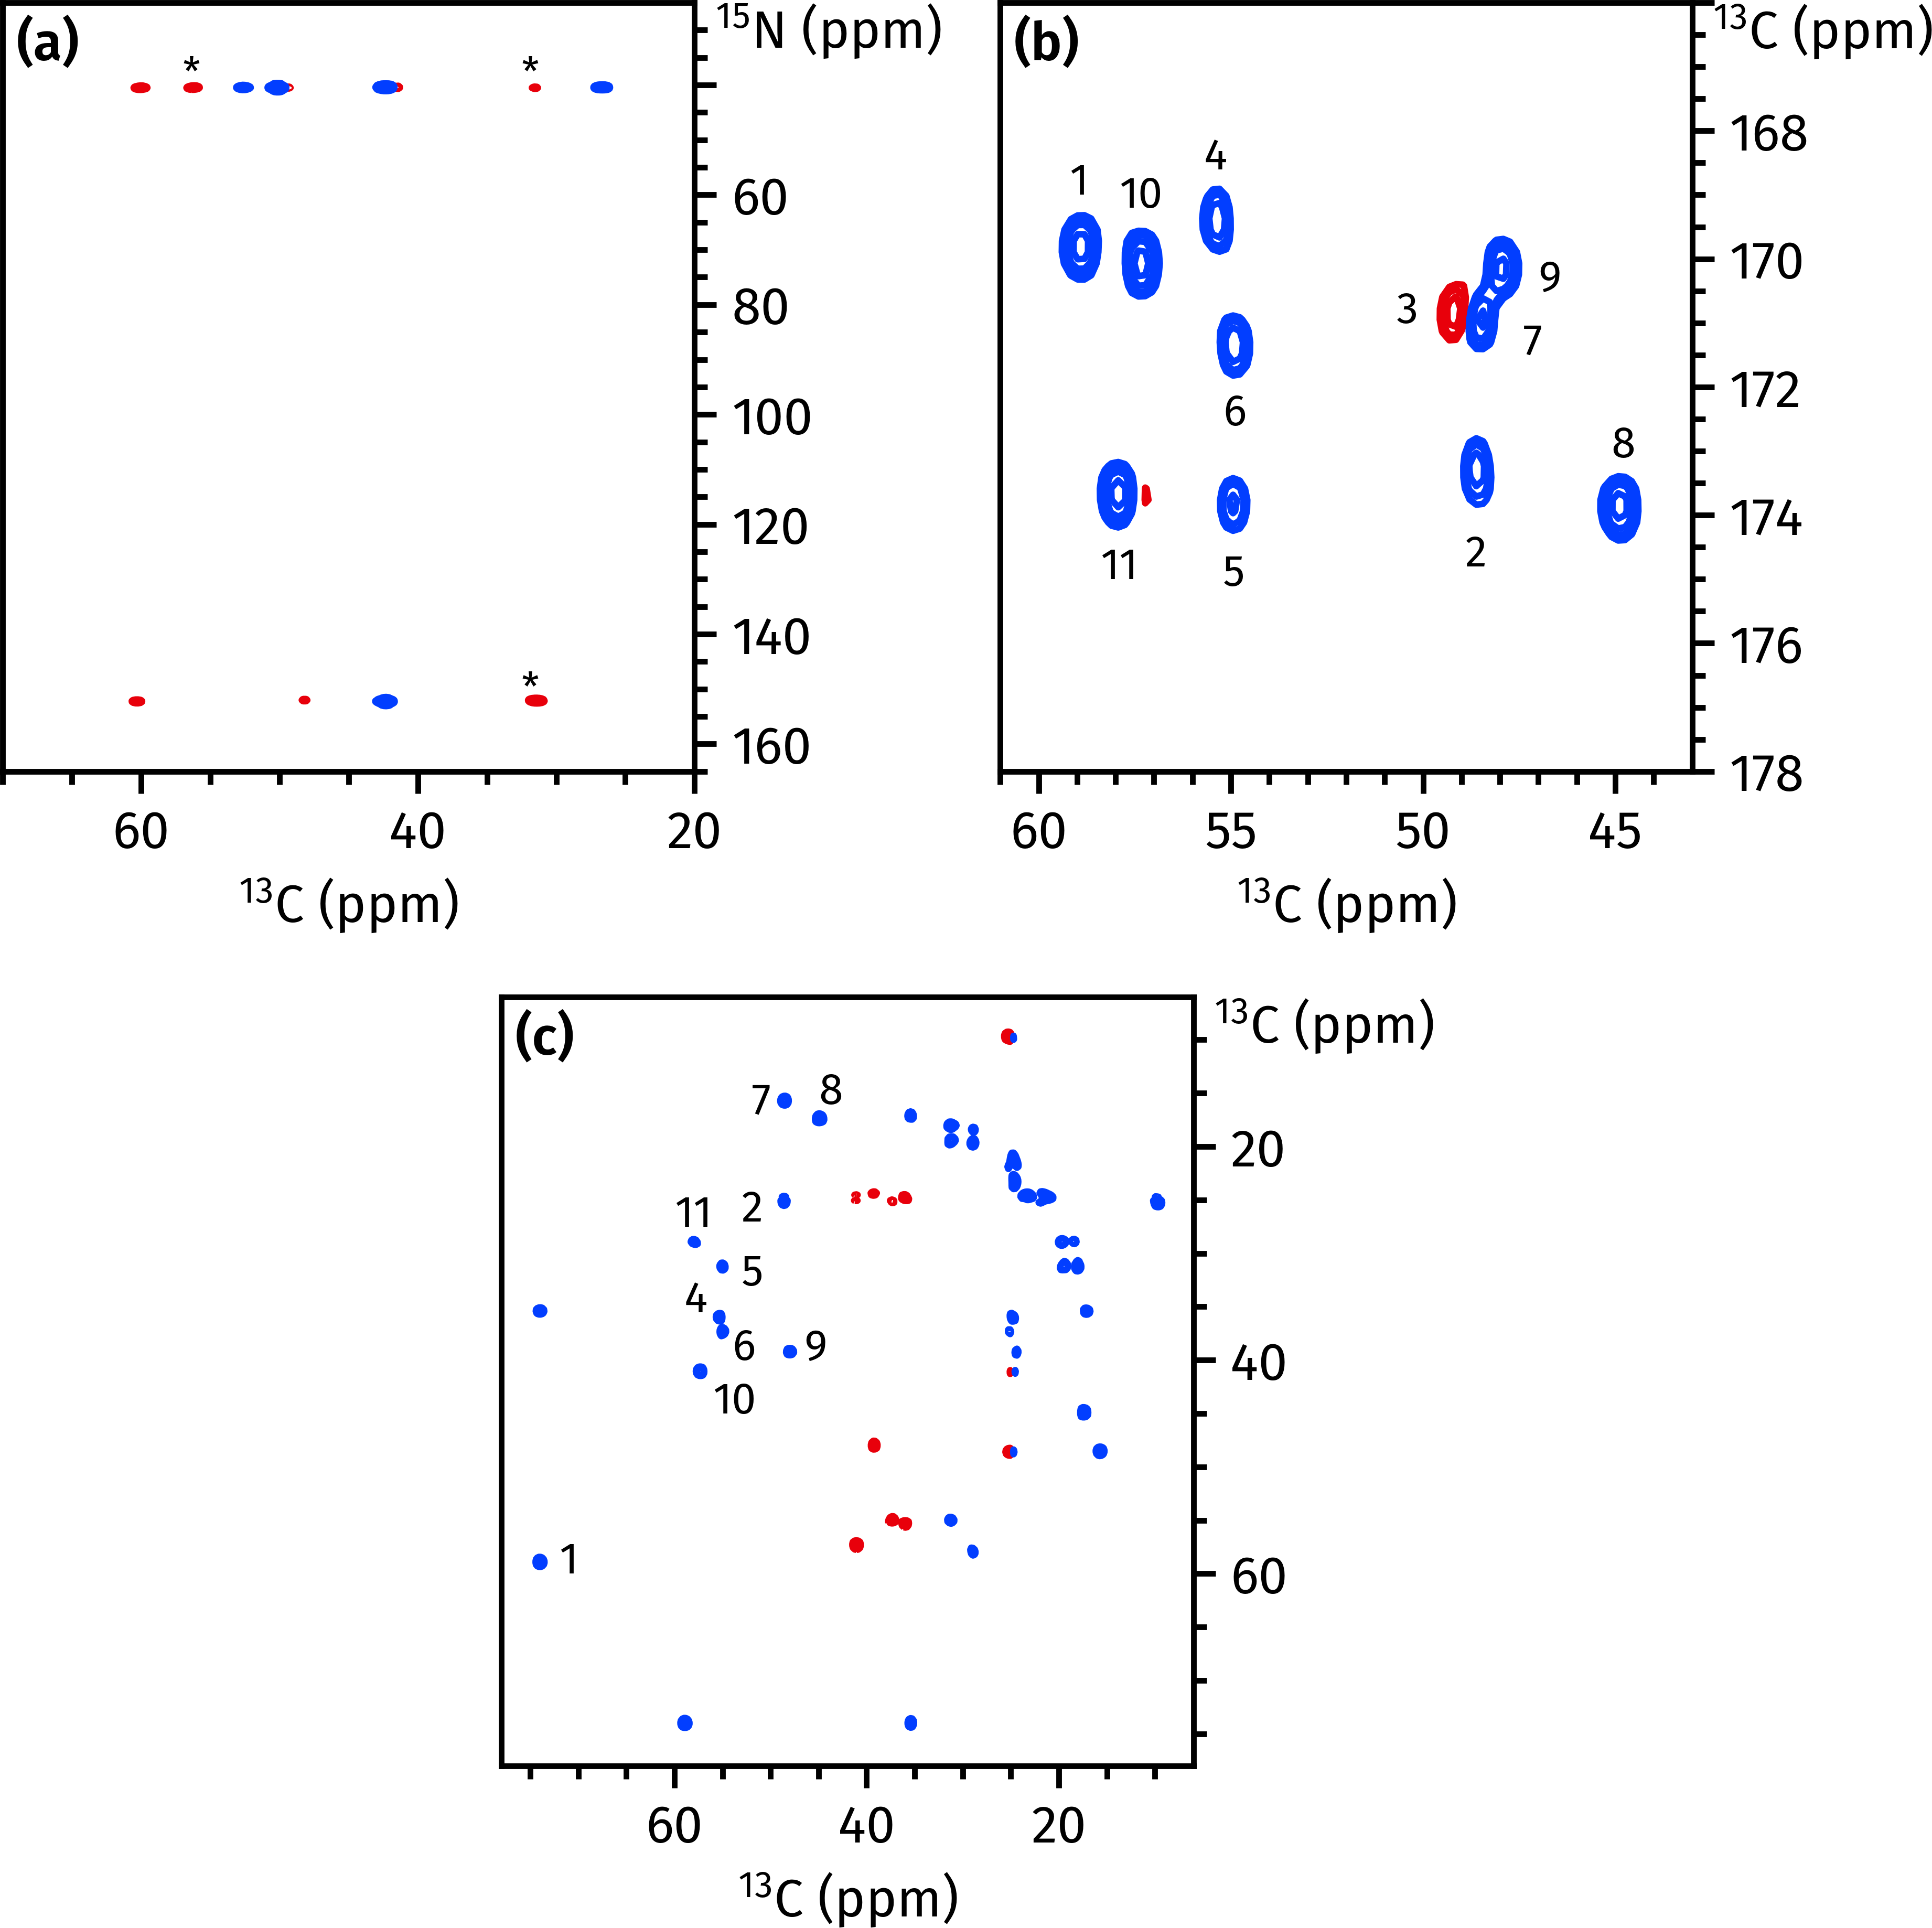
\includegraphics[]{covariance.png}%
    {\phantomsubcaption\label{fig:covariance_brucine_nc}}
    {\phantomsubcaption\label{fig:covariance_cyclo_caco}}
    {\phantomsubcaption\label{fig:covariance_cyclo_sidechain}}
    \caption{
        Spectra obtained through indirect covariance processing.
        In all cases the peak sign indicates carbon multiplicity; this information is contained in the multiplicity-edited \carbon{} HSQC spectrum and arises naturally during covariance processing.
        \textbf{(\subref*{fig:covariance_brucine_nc})} \carbon{}--\nitrogen{} correlation spectrum (containing both one- and multiple-bond correlations) obtained by processing the brucine \nitrogen{} HMBC and \carbon{} HSQC spectra (in \cref{fig:abbs_n_hmbc,fig:abbs_c_hsqc}) using unsymmetric indirect covariance.
        Some artefacts (arising from peak overlap in the \proton{} dimension) are marked with asterisks.
        \textbf{(\subref*{fig:covariance_cyclo_caco}--\subref*{fig:covariance_cyclo_sidechain})} Insets of \carbon{}--\carbon{} one-bond correlation spectrum, obtained by processing the cyclosporin ADEQUATE and \carbon{} HSQC spectra (in \cref{fig:abbss_adeq,fig:abbss_c_hsqc}) using generalised indirect covariance ($\lambda = 0.5$).
        The \ch{C}$\upalpha$--\ch{CO} correlations, numbered by residue (see \cref{fig:samples_cyclosporin}), are shown in (\subref*{fig:covariance_cyclo_caco}).
        Sidechain \ch{C-C} correlations are shown in (\subref*{fig:covariance_cyclo_sidechain}); only peaks corresponding to \ch{C}$\upalpha$--\ch{C}$\upbeta$ correlations are labelled.
        The inset in (\subref*{fig:covariance_cyclo_sidechain}) has been further subjected to a sign-preserving symmetrisation procedure, which is described in the text.
    }
    \label{fig:covariance}
\end{figure}

In \cref{fig:covariance_cyclo_sidechain}, the \carbon{}--\carbon{} one-bond covariance spectrum has been subjected to a sign-preserving symmetrisation procedure.
This is defined by replacing the intensity at each point $p(\Omega_1, \Omega_2)$ by
\begin{equation}
    \label{eq:covariance_symmetrisation}
    p(\Omega_1, \Omega_2) \to \sgn[p(\Omega_1, \Omega_2)] \cdot \min\left\{|p(\Omega_1, \Omega_2)|, |p(\Omega_2, \Omega_1)|\right\}.
\end{equation}
Here, $\sgn{p}$ refers to the sign of $p$, or equivalently $p / |p|$ (for $p \neq 0$).
The $\sgn{p}$ term ensures that the \textit{sign} of each peak (and hence multiplicity information) is preserved, but the (absolute) intensities are symmetrised about the main diagonal, which suppresses artefactual responses arising from coincidental peak overlap.

It should be noted that such a procedure can only be safely carried out where peaks on both sides of the diagonals are expected.
For a \textit{true} \carbon{}--\carbon{} correlation spectrum, this would be the case for all pairs of \carbon{} nuclei.
However, the covariance spectrum shown in \cref{fig:covariance_cyclo_caco,fig:covariance_cyclo_sidechain} does not satisfy this: peaks at $(\Omega_1, \Omega_2)$ are only observed if the carbon at $\Omega_2$ is bonded to at least one proton.
Thus, if the symmetrisation procedure is applied across the entire spectrum, correlations between quaternary and non-quaternary carbons (such as those in \cref{fig:covariance_cyclo_caco}) will be lost.
However, in the case of \cref{fig:covariance_cyclo_sidechain}, the alkyl region of cyclosporin does not contain any quaternary carbons, allowing the symmetrisation to be safely carried out.


\clearpage

\section{Software and raw data}

All processing was carried out using TopSpin 3 or 4.
Plots are generated in Python 3, using the \href{https://github.com/numpy/numpy}{\texttt{numpy}}, \href{https://github.com/scipy/scipy}{\texttt{scipy}}, and \href{https://github.com/yongrenjie/penguins}{\texttt{penguins}} libraries.
The raw data used for this paper, as well as all scripts required for regenerating the plots, are available on GitHub: \url{https://github.com/yongrenjie/abbs-paper}.

\subsection{Covariance}

The exact code used for covariance processing can be found in the \href{https://github.com/yongrenjie/abbs-paper/blob/main/figures/covariance.py}{\texttt{figures/covariance.py}} script.
A short overview is presented here.
The following code excerpt calculates the unsymmetric indirect covariance between two spectra.
Here, \texttt{penguins.read()} returns a \texttt{Dataset} object: the \texttt{rr} attribute of this is a two-dimensional \texttt{numpy} array corresponding to the doubly real part of the spectrum.

{\singlespacing
\begin{tcbminted}{python}
# Unsymmetric indirect covariance
import penguins as pg

spec1 = pg.read(path, expno1)
spec2 = pg.read(path, expno2)
cov = spec1.rr @ spec2.rr.T
\end{tcbminted}
}
\vspace{0.3cm}

Generalised indirect covariance is slightly more complicated, but follows directly from the procedure given in Snyder and Br\"uschweiler's work\autocite{Snyder2009JPCA}.

{\singlespacing
\begin{tcbminted}{python}
# Unsymmetric indirect covariance
import penguins as pg
import numpy as np
from scipy.linalg import fractional_matrix_power   # or just sqrtm

spec1 = pg.read(path, expno1)
spec2 = pg.read(path, expno2)
cov_lambda = 0.5

stacked = np.vstack((spec1.rr, spec2.rr))
cov_full = fractional_matrix_power(stacked @ stacked.T, cov_lambda)
# Figure out number of points in indirect dimensions of both spectra.
si1, si2 = spec1['si'][0], spec2['si'][0]
# `cov` is a block matrix, and we only want an off-diagonal block of it.
cov = np.real(cov_full[0:si1, si1:si1+si2)
\end{tcbminted}
}
\vspace{0.3cm}

Finally, this is the symmetrisation process specified in \cref{eq:covariance_symmetrisation}.
This assumes that the main diagonal of the \textit{spectrum} corresponds to the main diagonal of the \textit{matrix}, i.e.\ \texttt{m[i, i]} represents a point with the same chemical shift in both dimensions.
The matrix \texttt{cov} calculated above satisfies this.

{\singlespacing
\begin{tcbminted}{python}
import numpy as np

def symmetrise_preserve_sign(m):
    smallest_amp = np.minimum(np.abs(m), np.abs(m).T)
    sign = np.sign(m)
    return sign * smallest_amp
\end{tcbminted}
}

\clearpage

% Fakesection SI bibliography
\AtNextBibliography{\small}
\printbibliography{}
\clearpage    % For some reason this is needed to make the last page number 'S5', not '5'

\end{refsection}

\end{document}
